%%%%%%%%%%%%%%%%%%%%%%%%%%%%%%%%%%%%%%%%%%%%%%%%%%%
%% LaTeX book template                           %%
%% Author:  Amber Jain (http://amberj.devio.us/) %%
%% License: ISC license                          %%
%%%%%%%%%%%%%%%%%%%%%%%%%%%%%%%%%%%%%%%%%%%%%%%%%%%

\documentclass[a4paper,11pt,oneside]{book}
\usepackage{modulestyle}

%%%%%%%%%%%%%%%%%%%%%%%%%%%%%%%%%%%%%%%%%%%%%%%%%%%%%%%%%
% Source: http://en.wikibooks.org/wiki/LaTeX/Hyperlinks %
%%%%%%%%%%%%%%%%%%%%%%%%%%%%%%%%%%%%%%%%%%%%%%%%%%%%%%%%%

%%%%%%%%%%%%%%%%%%%%%%%%%%%%%%%%%%%%%%%%%%%%%%%%%%%%%%%%%%%%%%%%%%%%%%%%%%%%%%%%
% 'dedication' environment: To add a dedication paragraph at the start of book %
% Source: http://www.tug.org/pipermail/texhax/2010-June/015184.html            %
%%%%%%%%%%%%%%%%%%%%%%%%%%%%%%%%%%%%%%%%%%%%%%%%%%%%%%%%%%%%%%%%%%%%%%%%%%%%%%%%
\newenvironment{dedication}
{
   \cleardoublepage
   \thispagestyle{empty}
   \vspace*{\stretch{1}}
   \hfill\begin{minipage}[t]{0.66\textwidth}
   \raggedright
}
{
   \end{minipage}
   \vspace*{\stretch{3}}
   \clearpage
}

%%%%%%%%%%%%%%%%%%%%%%%%%%%%%%%%%%%%%%%%%%%%%%%%
% Chapter quote at the start of chapter        %
% Source: http://tex.stackexchange.com/a/53380 %
%%%%%%%%%%%%%%%%%%%%%%%%%%%%%%%%%%%%%%%%%%%%%%%%
\makeatletter
\renewcommand{\@chapapp}{}% Not necessary...
\newenvironment{chapquote}[2][2em]
  {\setlength{\@tempdima}{#1}%
   \def\chapquote@author{#2}%
   \parshape 1 \@tempdima \dimexpr\textwidth-2\@tempdima\relax%
   \itshape}
  {\par\normalfont\hfill--\ \chapquote@author\hspace*{\@tempdima}\par\bigskip}
\makeatother

%%%%%%%%%%%%%%%%%%%%%%%%%%%%%%%%%%%%%%%%%%%%%%%%%%%
% First page of book which contains 'stuff' like: %
%  - Book title, subtitle                         %
%  - Book author name                             %
%%%%%%%%%%%%%%%%%%%%%%%%%%%%%%%%%%%%%%%%%%%%%%%%%%%

\newcommand{\BookTitle}{Data Structures and Algorithms}
\newcommand{\BookTitleFootnote}{A course in the Bachelor of Science in Computer
Science/Information Technology/Information Systems program.}

\newcommand{\BookSubtitle}{A Study Guide for Students of Sorsogon State University - Bulan Campus}
\newcommand{\BookSubtitleFootnote}{This book is a study guide for students of
Sorsogon State University - Bulan Campus taking up the course Data Structures
and Algorithms.}

\newcommand{\BookAuthorFirstName}{Jarrian Vince}
\newcommand{\BookAuthorLastName}{Gojar}
\newcommand{\BookAuthorName}{Jarrian Vince G. Gojar}
\newcommand{\BookAuthorURL}{https://github.com/godkingjay}

% Book's title and subtitle
\title{\Huge \textbf{\BookTitle}  \footnote{\BookTitleFootnote} \\
\huge \BookSubtitle \footnote{\BookSubtitleFootnote}}

% Author
\author{\textsc{\BookAuthorName}\thanks{\url{\BookAuthorURL}}}

\begin{document}

\frontmatter
\maketitle

%%%%%%%%%%%%%%%%%%%%%%%%%%%%%%%%%%%%%%%%%%%%%%%%%%%%%%%%%%%%%%%
% Add a dedication paragraph to dedicate your book to someone %
%%%%%%%%%%%%%%%%%%%%%%%%%%%%%%%%%%%%%%%%%%%%%%%%%%%%%%%%%%%%%%%
\begin{dedication}
Sorsogon State University - Bulan Campus
\end{dedication}

%%%%%%%%%%%%%%%%%%%%%%%%%%%%%%%%%%%%%%%%%%%%%%%%%%%%%%%%%%%%%%%%%%%%%%%%
% Auto-generated table of contents, list of figures and list of tables %
%%%%%%%%%%%%%%%%%%%%%%%%%%%%%%%%%%%%%%%%%%%%%%%%%%%%%%%%%%%%%%%%%%%%%%%%
\tableofcontents
\listoffigures
\listoftables
\lstlistoflistings

\mainmatter

%%%%%%%%%%%
% Preface %
%%%%%%%%%%%
\chapter*{Preface}
% A Quote all about Data Structures and Algorithms
\begin{chapquote}{Linus Torvalds}
``Bad programmers worry about the code. Good programmers worry about data structures and their relationships.''
\end{chapquote}

\noindent \BookAuthorName \\
\noindent \url{\BookAuthorURL}

%%%%%%%%%%%%%%%%%%%%%%%%%%%%%%%%%%%%
%%%%%~ NEW CHAPTER STARTS HERE %%%%%
%%%%%%%%%%%%%%%%%%%%%%%%%%%%%%%%%%%%
\chapter{Introduction to Data Structures and Algorithms}

\section{Introduction}

Data structures and algorithms are one of the fundamental components of computer
science. They are essential for solving complex problems efficiently and
effectively. Data structures are used to store and organize data in a computer
so that it can be accessed and manipulated efficiently. Algorithms
are step-by-step procedures or formulas for solving a problem. They are the
instructions that tell a computer how to perform a task.

In this course, we will learn about the fundamental data structures and
algorithms that are used in computers. We will study how to design,
implement, and analyze data structures and algorithms to solve real-world
problems. By the end of this course, you will have a solid foundation in
data structures and algorithms that will help you become a better programmer
and problem solver.

\section{Setup and Installation}

In this course, we will be using the C++ programming language to implement
data structures and algorithms. C++ is a powerful and versatile programming
language that is widely used in the field of computer science. To get started,
you will need to install a C++ compiler and an integrated development
environment (IDE) on your computer.

\subsection{C++ Compiler Installation}

The first step is to install a C++ compiler on your computer. A compiler is
a program that translates source code written in a programming language into
machine code that can be executed by a computer. There are several C++
compilers available, but we recommend using the GNU Compiler Collection (GCC)
which is a free and open-source compiler that supports multiple programming
languages including C++.

\subsubsection{Windows}

To install GCC on Windows, you can use the MinGW (Minimalist GNU for Windows)
project which provides a port of GCC to Windows. You can download the MinGW
installer from the MinGW website and follow the installation instructions.
You can install MinGW by following the instructions here:
\url{https://code.visualstudio.com/docs/languages/cpp#_example-install-mingwx64-on-windows}

\subsection{Visual Studio Code Installation}

The next step is to install an integrated development environment (IDE) on
your computer. An IDE is a software application that provides comprehensive
facilities to computer programmers for software development. We recommend
using Visual Studio Code which is a free and open-source IDE developed by
Microsoft. You can download Visual Studio Code from the official website
and follow the installation instructions: \url{https://code.visualstudio.com/Download}

Other than Visual Studio Code, you also need to install the C/C++ extension
for Visual Studio Code. You can install the C/C++ extension by following the
instructions here: \url{https://code.visualstudio.com/docs/languages/cpp}

\subsection{Testing the Installation}

To test if the installation was successful, you can create a simple C++
program and compile it using the C++ compiler. Open Visual Studio Code and
create a new file with the following C++ code:

\begin{lstlisting}[language=C++, caption={Hello World Program}]
#include <iostream>
namespace std;

int main() {
    cout << "Hello, World!" << endl;
    return 0;
}
\end{lstlisting}

Save the file with a .cpp extension (e.g., hello.cpp) and open a terminal
window in Visual Studio Code. Compile the program using the following command:

\begin{lstlisting}[language=bash, caption={Compiling the Program}]
g++ hello.cpp -o hello
\end{lstlisting}

If there are no errors, you can run the program by executing the following
command:

\begin{lstlisting}[language=bash, caption={Running the Program}]
./hello
\end{lstlisting}

If everything is set up correctly, you should see the output "Hello, World!"
printed on the screen.

\section{What are Data Structures?}

A \textbf{\textit{data structure}} is a way of organizing and storing data in a computer so
that it can be accessed and manipulated efficiently. Data structures provide a
way to manage large amounts of data effectively for various applications. They
define the relationship between the data, and the operations that can be
performed on the data. There are many different types of data structures that
are used in computer science, each with its own strengths and weaknesses. The use
of the right data structure can significantly improve the performance of an
algorithm and make it more efficient.

\section{What are Algorithms?}

An \textbf{\textit{algorithm}} is a step-by-step procedure or formula for solving a problem.
It is a sequence of well-defined instructions that take some input and produce
an output. Algorithms are used to solve complex problems and perform various
tasks efficiently. They are the instructions that tell a computer how to perform
a task. Algorithms are essential for writing computer programs and developing
software applications. The efficiency of an algorithm is measured by its time
complexity and space complexity.

\section{Why Study Data Structures and Algorithms?}

Data structures and algorithms are essential topics in computer science and
software engineering. They are one of the fundamental components of computer
science and are used in various applications such as operating systems,
database management systems, networking, artificial intelligence, and many
others. A good understanding of data structures and algorithms will help
you become a better programmer and problem solver. In addition, many companies
use data structures and algorithms as part of their technical interviews to
assess the problem-solving skills of candidates. Therefore, studying data
structures and algorithms is essential for anyone pursuing a career in
software engineering or software development.

\section{Basic Terminologies}

Before we dive into the details of data structures and algorithms, let's
understand some basic terminologies that might be helpful in understanding
the concepts better.

\subsection{Data}

\textbf{\textit{Data}} is a collection of facts, figures, or information that
can be used for analysis or reference. It can be in the form of numbers, text,
images, audio, video, or any other format. Data is the raw material that is
processed by a computer to produce meaningful information.

\subsection{Data Object}

A \textbf{\textit{data object}} is an instance of a data structure that contains
data along with the operations that can be performed on the data. It is an
abstraction of a real-world entity that is represented in a computer program.

\subsection{Data Type}

A \textbf{\textit{data type}} is a classification of data that tells the compiler
or interpreter how the programmer intends to use the data. It defines the
operations that can be performed on the data, the values that can be stored
in the data, and the memory space required to store the data.

\subsubsection{Primitive Data Types}

Primitive data types are the basic data types that are built into the programming
language. They are used to store simple values such as integers, floating-point
numbers, characters, and booleans. Examples of primitive data types include
int, float, char, and bool. The following are the common primitive data types
used in programming:

\paragraph{Integer (int)}

The \textbf{\textit{integer}} data type is used to store whole numbers without any decimal points.
It can be either signed or unsigned, depending on whether it can store negative
values or not. An integer's value can range from -2,147,483,648 to 2,147,483,647
and takes 4 bytes of memory.

\begin{lstlisting}[language=C++, caption={Integer Data Type}]
int x = 10;
\end{lstlisting}


\paragraph{Character (char)}

The \textbf{\textit{character}} data type is used to store a single character such as a letter,
digit, or special symbol. It is represented by a single byte of memory. A char
value can range from -128 to 127 or 0 to 255, depending on whether it is signed
or unsigned. These values are represented using ASCII codes.

\begin{lstlisting}[language=C++, caption={Character Data Type}]
char c = 'A';
\end{lstlisting}

\paragraph{Boolean (bool)}

The \textbf{\textit{boolean}} data type is used to store true or false values. It is represented
by a single byte of memory. A bool value can be either true or false.

\begin{lstlisting}[language=C++, caption={Boolean Data Type}]
bool flag = true;
\end{lstlisting}

\paragraph{Floating-Point (float)}

The \textbf{\textit{floating-point}} data type is used to store real numbers with decimal points.
It can represent both integer and fractional parts of a number. It can be either
single precision or double precision, depending on the number of bits used to
store the value. A float value can range from 1.2E-38 to 3.4E+38 and takes 4
bytes of memory.

\begin{lstlisting}[language=C++, caption={Floating-Point Data Type}]
float y = 3.14;
\end{lstlisting}

\paragraph{Double (double)}

The \textbf{\textit{double}} data type is used to store real numbers with double precision. It can
represent both integer and fractional parts of a number with higher precision
than the float data type. A double value can range from 2.3E-308 to 1.7E+308 and
takes 8 bytes of memory.

\begin{lstlisting}[language=C++, caption={Double Data Type}]
double z = 3.14159;
\end{lstlisting}

\subsubsection{Non-primitive Data Types}

Non-primitive data types are more complex data types that are derived from primitive
data types. They are used to store collections of values or objects. Examples of
non-primitive data types include arrays, strings, structures, classes, and pointers.

\paragraph{Array (int, float, char, etc.)}

An \textbf{\textit{array}} is a collection of elements of the same data type that are stored in
contiguous memory locations. It is used to store multiple values of the same
type under a single name. The elements of an array can be accessed using an
index value. In C++, arrays are zero-indexed, which means the first element is
at index 0. Arrays also have a fixed size that is specified at the time of
declaration. If you need a dynamic size array, you can use a vector in C++.

\begin{lstlisting}[language=C++, caption={Array Data Type}]
int arr[5] = {1, 2, 3, 4, 5};
\end{lstlisting}

\paragraph{String (char)}

A \textbf{\textit{string}} is a collection of characters that are stored
as a sequence of characters terminated by a null character
'\textbackslash0'. It is used to represent text in a computer program.
Strings are treated as arrays of characters in C++.

\begin{lstlisting}[language=C++, caption={String Data Type}]
char str[] = "Hello, World!";
\end{lstlisting}

\paragraph{Structure}

A \textbf{\textit{structure}} is a user-defined data type that is used to
store a collection of different data types under a single name. It is used
to represent a record that contains multiple fields or members. Each field
in a structure can have a different data type.

\begin{lstlisting}[language=C++, caption={Structure Data Type}]
struct Person {
    char name[50];
    int age;
    float height;
};
\end{lstlisting}

\paragraph{Class}

A \textbf{\textit{class}} is a user-defined data type that is used to define
objects that contain data members and member functions. It is used to
implement object-oriented programming concepts such as encapsulation,
inheritance, and polymorphism.

\begin{lstlisting}[language=C++, caption={Class Data Type}]
class Circle {
    private:
        float radius;
    public:
        float getArea() {
            return 3.14 * radius * radius;
        }
};
\end{lstlisting}

% \paragraph{Pointer}

% A \textbf{\textit{pointer}} is a special type of data type that stores the
% memory address of another data type. It is used to store the address of a
% variable or object in memory. Pointers are used to implement dynamic
% memory allocation and to pass parameters by reference.

% \begin{lstlisting}[language=C++, caption={Pointer Data Type}]
% int x = 10;
% int *ptr = &x;

% cout << *ptr; // Output: 10
% \end{lstlisting}

\paragraph{Vector}

A \textbf{\textit{vector}} is a dynamic array that can grow or shrink in size
dynamically. It is a part of the Standard Template Library (STL) in C++ and
provides a more flexible alternative to fixed-size arrays. Vectors are used
to store a collection of elements of the same data type.

\begin{lstlisting}[language=C++, caption={Vector Data Type}]
vector<int> vec = {1, 2, 3, 4, 5};
\end{lstlisting}

\paragraph{List}

A \textbf{\textit{list}} is a linear data structure that is used to store a
collection of elements in a sequential order. It is a part of the Standard
Template Library (STL) in C++ and provides operations to insert, delete, and
access elements in the list. Lists are used to implement linked lists in C++.

\begin{lstlisting}[language=C++, caption={List Data Type}]
list<int> lst = {1, 2, 3, 4, 5};
\end{lstlisting}

There are different types of lists in C++, such as singly linked list, doubly
linked list, circular linked list, and circular doubly linked list, that provide different operations and
performance characteristics.

\subparagraph{Singly Linked List}

A \textbf{\textit{singly linked list}} is a linear data structure that is used
to store a collection of elements in a sequential order. Each element in the
list is stored in a node that contains the data and a pointer to the next node
in the list.

\begin{lstlisting}[language=C++, caption={Singly Linked List Data Type}]
struct Node {
    int data;
    Node *next;
};
\end{lstlisting}

\subparagraph{Doubly Linked List}

A \textbf{\textit{doubly linked list}} is a linear data structure that is used
to store a collection of elements in a sequential order. Each element in the
list is stored in a node that contains the data, a pointer to the next node,
and a pointer to the previous node in the list.

\begin{lstlisting}[language=C++, caption={Doubly Linked List Data Type}]
struct Node {
    int data;
    Node *next;
    Node *prev;
};
\end{lstlisting}

\subparagraph{Circular Linked List}

A \textbf{\textit{circular linked list}} is a linear data structure that is used
to store a collection of elements in a circular order. Each element in the list
is stored in a node that contains the data and a pointer to the next node in
the list. The last node in the list points back to the first node, creating a
circular structure.

\begin{lstlisting}[language=C++, caption={Circular Linked List Data Type}]
struct Node {
    int data;
    Node *next;
};
\end{lstlisting}

\subparagraph{Circular Doubly Linked List}

A \textbf{\textit{circular doubly linked list}} is a linear data structure that
is used to store a collection of elements in a circular order. Each element in
the list is stored in a node that contains the data, a pointer to the next node,
and a pointer to the previous node in the list. The last node in the list points
back to the first node, creating a circular structure.

\begin{lstlisting}[language=C++, caption={Circular Doubly Linked List Data Type}]
struct Node {
    int data;
    Node *next;
    Node *prev;
};
\end{lstlisting}

\paragraph{Stack}

A \textbf{\textit{stack}} is a linear data structure that follows the Last In
First Out (LIFO) principle. It is used to store a collection of elements in a
sequential order. The main operations on a stack are push (to insert an element)
and pop (to remove an element).

\begin{lstlisting}[language=C++, caption={Stack Data Type}]
stack<int> stk;
stk.push(1);
stk.push(2);
stk.push(3);
stk.push(4);
stk.pop();
\end{lstlisting}

\paragraph{Queue}

A \textbf{\textit{queue}} is a linear data structure that follows the First In
First Out (FIFO) principle. It is used to store a collection of elements in a
sequential order. The main operations on a queue are enqueue (to insert an
element) and dequeue (to remove an element).

\begin{lstlisting}[language=C++, caption={Queue Data Type}]
queue<int> que;
que.push(1);
que.push(2);
que.push(3);
que.push(4);
que.pop();
\end{lstlisting}

There are different types of queues in C++, such as linear queue, circular
queue, priority queue, and double-ended queue (deque), that provide different
operations and performance characteristics.

\subparagraph{Circular Queue}

A \textbf{\textit{circular queue}} is a type of queue that uses a circular
structure to store elements. Unlike a linear queue, a circular queue does not
have a fixed front and rear end. Instead, the front and rear ends wrap around
the ends of the queue. This allows the queue to reuse the space freed up by
dequeued elements. In C++, there is no built-in circular queue data type, but
you can implement one using an array and a few pointers.

\subparagraph{Priority Queue}

A \textbf{\textit{priority queue}} is a type of queue that stores elements
based on their priority. The element with the highest priority is dequeued
first. Priority queues are typically implemented using heaps, which are a
type of binary tree data structure.

\begin{lstlisting}[language=C++, caption={Priority Queue Data Type}]
priority_queue<int> pq;
pq.push(1);
pq.push(4);
pq.push(2);
pq.push(3);
pq.pop();
\end{lstlisting}

\subparagraph{Double-Ended Queue (Deque)}

A \textbf{\textit{double-ended queue}} or \textbf{\textit{deque}} is a type of
queue that allows elements to be inserted and removed from both ends. It is
a generalization of both stacks and queues and provides more flexibility in
manipulating elements.

\begin{lstlisting}[language=C++, caption={Deque Data Type}]
deque<int> dq;
dq.push_front(1);
dq.push_back(2);
dq.push_front(3);
dq.push_back(4);
dq.pop_front();
\end{lstlisting}

\paragraph{Tree}

A \textbf{\textit{tree}} is a non-linear data structure that is used to store
a collection of elements in a hierarchical order. It consists of nodes that
are connected by edges. The topmost node in a tree is called the root node,
and the nodes below it are called child nodes. Trees are used to represent
hierarchical relationships between elements.

\begin{lstlisting}[language=C++, caption={Tree Data Type}]
struct Node {
    int data;
    Node *left;
    Node *right;
};
\end{lstlisting}

There are different types of trees in computer science, such as binary trees,
binary search trees, AVL trees, red-black trees, and many others, that provide
different operations and performance characteristics.

\paragraph{Graph}

A \textbf{\textit{graph}} is a non-linear data structure that is used to store
a collection of elements and the relationships between them. It consists of
nodes (vertices) that are connected by edges. Graphs are used to represent
networks, social relationships, maps, and many other real-world applications.

\begin{lstlisting}[language=C++, caption={Graph Data Type}]
struct Graph {
    int V;
    list<int> *adj;
};
\end{lstlisting}

There are different types of graphs in computer science, such as directed graphs,
undirected graphs, weighted graphs, and many others, each with its own set of
advantages and disadvantages.

Another important thing to note is that ``Every tree is a graph, but not every
graph is a tree.''

\paragraph{Hash Map or Hash Table}

A \textbf{\textit{Hash Map}} is a data structure that is used to store a
collection of key-value pairs. It uses a hash function to map keys to values
and stores them in an array. Hash maps provide fast access to elements and
are used to implement associative arrays, sets, and dictionaries.

There are two ways to implement a hash map in C++: the ordered map using the
map class or using the unordered\_map class.

\begin{lstlisting}[language=C++, caption={Ordered Map Data Type}]
map<string, int> mp;
mp["one"] = 1;
mp["two"] = 2;
mp["three"] = 3;
\end{lstlisting}

\begin{lstlisting}[language=C++, caption={Unordered Map Data Type}]
unordered_map<string, int> ump;
ump["one"] = 1;
ump["two"] = 2;
ump["three"] = 3;
\end{lstlisting}

\paragraph{Set}

A \textbf{\textit{set}} is a data structure that is used to store a collection
of unique elements. It is used to implement the mathematical set abstraction
and provides operations to insert, delete, and search for elements.

There are two ways to implement a set in C++: the ordered set using the set
class or using the unordered\_set class.

\begin{lstlisting}[language=C++, caption={Ordered Set Data Type}]
set<int> st;
st.insert(1);
st.insert(2);
st.insert(3);
\end{lstlisting}

\begin{lstlisting}[language=C++, caption={Unordered Set Data Type}]
unordered_set<int> ust;
ust.insert(1);
ust.insert(2);
ust.insert(3);
\end{lstlisting}

\subsection{Abstract Data Type}

An \textbf{\textit{abstract data type (ADT)}} is a mathematical model that
defines a set of data values and operations that can be performed on those
values. It is an abstraction of a data structure that specifies the operations
that can be performed on the data without specifying how they are implemented.
\textit{Abstraction} refers to the process of hiding the implementation
details of a data structure and exposing only the essential features. An ADT
is defined by its interface, which includes the data values and operations
that can be performed on those values.

\subsection{Pointers}

A \textbf{\textit{pointer}} is a special type of data type that stores the
memory address of another data type. An ``address'' is a unique number that
identifies a location in memory. The memory address of a variable is the
location in memory where the variable is stored. Pointers are used to store
the address of a variable or object in memory. Pointers are used to implement
dynamic memory allocation and to pass parameters by reference.

\begin{figure}[h]
    \centering
    \begin{tikzpicture}
        \node (x) [draw, rectangle] {x = 10};
        \node (ptr) [draw, rectangle, right=of x] {ptr = 0x7fffbf7f1bdc};
        \draw[->] (ptr) -- (x);
    \end{tikzpicture}
    \caption{Pointer Example}
    \label{fig:pointer-example}
\end{figure}

Figure \ref{fig:pointer-example} shows an example of a pointer in C++. The
variable \texttt{x} stores the value 10, and the pointer \texttt{ptr} stores
the memory address of the variable \texttt{x}. The memory address is represented
as a hexadecimal number \texttt{0x7fffbf7f1bdc}.

\begin{lstlisting}[language=C++, caption={Pointer Data Type}]
int main() {
    int x = 10;
    int *ptr = &x;

    cout << *ptr; // Output: 10

    return 0;
}
\end{lstlisting}

In the above example, the pointer \texttt{ptr} stores the memory address of
the variable \texttt{x}. The \texttt{*} operator is used to dereference the
pointer and access the value stored at the memory address.

An example of an address of a variable is \texttt{0x7fffbf7f1bdc}. When you
dereference the pointer, you get the value stored at that address.

\subsubsection{Declaring Pointers}

To declare a pointer, you need to specify the data type of the variable or
object it points to. You can declare a pointer using the following syntax:

\begin{lstlisting}[language=C++, caption={Declaring Pointers}]
int *ptr;
\end{lstlisting}

In the above example, the pointer \texttt{ptr} is declared to point to an
integer variable. You can also declare a pointer to a structure, class, or
any other data type.

\subsubsection{Initializing Pointers}

To initialize a pointer, you need to assign it the memory address of a variable
or object. You can initialize a pointer using the address-of operator \texttt{\&}.
You can also initialize a pointer to \texttt{NULL} or \texttt{nullptr} to indicate
that it does not point to any memory location.

\begin{lstlisting}[language=C++, caption={Initializing Pointers}]
int x = 10;
int *ptr = &x;
\end{lstlisting}

In the above example, the pointer \texttt{ptr} is initialized with the memory
address of the variable \texttt{x}.

\subsubsection{Dereferencing Pointers}

To access the value stored at the memory address pointed to by a pointer, you
need to dereference the pointer using the dereference operator \texttt{*}. The
dereference operator is used to access the value stored at the memory address.

% Create a tikz figure for dereferencing pointers
\begin{figure}[h]
    \centering
    \begin{tikzpicture}
        \node (x) [draw, rectangle] {x = 10};
        \node (ptr) [draw, rectangle, right=of x] {ptr = 0x7fffbf7f1bdc};
        \draw[->] (ptr) -- (x);
        \node (value) [draw, rectangle, below=of ptr] {*ptr = 10};
        \draw[dashed] (value) -- (ptr);
        \draw[->] (value) -- (x);
    \end{tikzpicture}
    \caption{Dereferencing Pointers}
    \label{fig:dereferencing-pointers}
\end{figure}

Figure \ref{fig:dereferencing-pointers} shows an example of dereferencing a
pointer in C++. The pointer \texttt{ptr} points to the variable \texttt{x},
and the dereference operator \texttt{*} is used to access the value stored at
the memory address.

\begin{lstlisting}[language=C++, caption={Dereferencing Pointers}]
int x = 10;
int *ptr = &x;

cout << *ptr; // Output: 10

*ptr = 20;

cout << x; // Output: 20

\end{lstlisting}

In the above example, the pointer \texttt{ptr} points to the variable \texttt{x}.
You can use the dereference operator \texttt{*} to access the value stored at
the memory address. You can also use the dereference operator to modify the
value stored at the memory address.

\subsubsection{Pointer Arithmetic}

Pointer arithmetic is a feature of pointers that allows you to perform
arithmetic operations on pointers. You can add or subtract an integer value
from a pointer to move it to a different memory location. Pointer arithmetic
is used to access elements in an array or to iterate over a data structure.

\begin{figure}[h]
    \centering
    \begin{tikzpicture}
        \node (arr) [draw, rectangle] {arr = [1, 2, 3, 4, 5]};
        \node (ptr) [draw, rectangle, right=of arr] {ptr = 0x7fffbf7f1bdc};
        \draw[->] (ptr) -- (arr);
        \node (value) [draw, rectangle, below=of ptr] {*(ptr + 1) = 2};
        \draw[dashed] (value) -- (ptr);
        \draw[->] (value) -- (arr);
    \end{tikzpicture}
    \caption{Pointer Arithmetic}
    \label{fig:pointer-arithmetic}
\end{figure}

Figure \ref{fig:pointer-arithmetic} shows an example of pointer arithmetic in C++.
The pointer \texttt{ptr} points to the first element of the array \texttt{arr},
and the pointer arithmetic operation \texttt{*(ptr + 1)} is used to access the
second element of the array.

\begin{lstlisting}[language=C++, caption={Pointer Arithmetic}]
int main() {
    int arr[5] = {1, 2, 3, 4, 5};
    int *ptr = arr;

    cout << *ptr; // Output: 1
    cout << *(ptr + 1); // Output: 2

    return 0;
}
\end{lstlisting}

In the above example, the pointer \texttt{ptr} points to the first element
of the array \texttt{arr}. You can use pointer arithmetic to access the
elements of the array by adding an integer value to the pointer.

\subsubsection{Pointer to Pointer}

A \textbf{\textit{pointer to pointer}} is a special type of pointer that stores
the memory address of another pointer. It is used to store the address of a
pointer variable in memory. Pointer to pointer is used to implement multiple
levels of indirection and to create dynamic data structures such as linked
lists and trees.

% Create a tikz figure for pointer to pointer

\begin{figure}[h]
    \centering
    \begin{tikzpicture}
        \node (x) [draw, rectangle] {x = 10};
        \node (ptr) [draw, rectangle, right=of x] {ptr = 0x7fffbf7f1bdc};
        \draw[->] (ptr) -- (x);
        \node (pptr) [draw, rectangle, right=of ptr] {pptr = 0x7fffbf7f1be0};
        \draw[->] (pptr) -- (ptr);
        \node (value) [draw, rectangle, below=of pptr] {**pptr = 10};
        \draw[dashed] (value) -- (pptr);
        \draw[->] (value) -- (x);
    \end{tikzpicture}
    \caption{Pointer to Pointer}
    \label{fig:pointer-to-pointer}
\end{figure}

Figure \ref{fig:pointer-to-pointer} shows an example of a pointer to pointer in C++.
The pointer \texttt{ptr} stores the memory address of the variable \texttt{x},
and the pointer \texttt{pptr} stores the memory address of the pointer \texttt{ptr}.
The double dereference operator \texttt{**} is used to access the value stored at
the memory address.

\begin{lstlisting}[language=C++, caption={Pointer to Pointer Data Type}]
int main() {
    int x = 10;
    int *ptr = &x;
    int **pptr = &ptr;

    cout << **pptr; // Output: 10

    return 0;
}
\end{lstlisting}

In the above example, the pointer \texttt{ptr} stores the memory address of
the variable \texttt{x}, and the pointer \texttt{pptr} stores the memory
address of the pointer \texttt{ptr}. You can use the double dereference
operator \texttt{**} to access the value stored at the memory address.

\section{Asymptotic Notations}

\textbf{\textit{Asymptotic notations}} are mathematical notations used to
describe the limiting behavior of a function as the input size approaches
infinity. They are used to analyze the complexity of algorithms and to
compare the performance of different algorithms. The three most common
asymptotic notations used in computer science are big-O notation, omega
notation, and theta notation.

\begin{figure}[h]
  \centering
  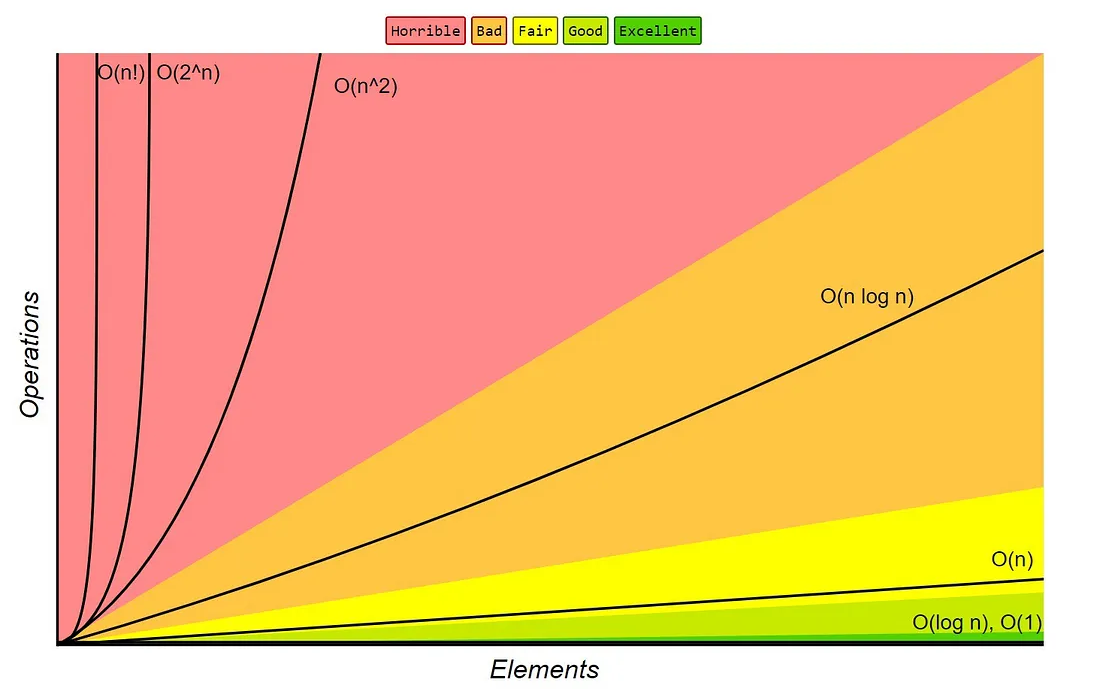
\includegraphics[width=0.6\textwidth]{./assets/images/Asymptotic Notations.png}
  \caption{Asymptotic Notation}
  \floatfoot{Big-O Complexity Analysis Chart from freeCodeCamp}
\end{figure}

\subsection{Big-O Notation}

The \textbf{\textit{big-O notation}} is used to describe the upper bound
on the growth rate of an algorithm as the input size approaches infinity.
It provides an upper limit on the worst-case time complexity of an algorithm.
The big-O notation is used to analyze the efficiency of an algorithm in terms
of the number of basic operations it performs.

\subsection{Omega Notation}

The \textbf{\textit{omega notation}} or \textbf{\textit{big-omega notation}}
is used to describe the lower bound on the growth rate of an algorithm as the
input size approaches infinity. It provides a lower limit on the best-case
time complexity of an algorithm. The omega notation is used to analyze the
efficiency of an algorithm in terms of the minimum number of basic operations
it performs.

\subsection{Theta Notation}

The \textbf{\textit{theta notation}} or \textbf{\textit{big-theta notation}}
is used to describe the tight bound on the growth rate of an algorithm as
the input size approaches infinity. It provides an upper and lower limit on
the time complexity of an algorithm. The theta notation is used to analyze
the efficiency of an algorithm in terms of the average number of basic
operations it performs.

\subsection{Complexity of an Algorithm}

The \textbf{\textit{complexity of an algorithm}} is a measure of the amount of time and
space required to execute the algorithm as a function of the input size. It is used
to analyze the efficiency of an algorithm and to compare different algorithms for
the same problem. The complexity of an algorithm is usually expressed using big-O
notation, which provides an upper bound on the growth rate of the algorithm as the
input size increases.

\subsubsection{Time Complexity}

The \textbf{\textit{time complexity}} of an algorithm is a measure of the amount of time
required to execute the algorithm as a function of the input size. It is used to
analyze the efficiency of an algorithm in terms of the number of basic operations
it performs. The time complexity of an algorithm is usually expressed using big-O
notation, which provides an upper bound on the growth rate of the algorithm as the
input size increases.

\paragraph{Constant Time Complexity ($O(1)$)}

An algorithm is said to have a \textbf{\textit{constant time complexity}} if the
execution time of the algorithm does not depend on the input size. It means
that the algorithm takes the same amount of time to execute regardless of
the input size. An example of an algorithm with constant time complexity is
accessing an element in an array using its index.

\begin{lstlisting}[language=C++, caption={Constant Time Complexity}]
int arr[5] = {1, 2, 3, 4, 5};
int x = arr[2]; // Accessing the element at index 2
\end{lstlisting}

\paragraph{Logarithmic Time Complexity ($O(\log n)$)}

An algorithm is said to have a \textbf{\textit{logarithmic time complexity}} if
the execution time of the algorithm grows logarithmically as the input size
increases. An example of an algorithm with logarithmic time complexity is
binary search, where the input size is halved at each step.

\begin{lstlisting}[language=C++, caption={Logarithmic Time Complexity}]
int binarySearch(int arr[], int n, int x) {
    int low = 0, high = n - 1;
    while (low <= high) {
        int mid = low + (high - low) / 2;
        if (arr[mid] == x) return mid;
        else if (arr[mid] < x) low = mid + 1;
        else high = mid - 1;
    }
    return -1;
}
\end{lstlisting}

\paragraph{Linear Time Complexity ($O(n)$)}

An algorithm is said to have a \textbf{\textit{linear time complexity}} if the
execution time of the algorithm grows linearly as the input size increases.
It means that the algorithm takes a constant amount of time to process each
element in the input. An example of an algorithm with linear time complexity
is traversing an array to find the maximum element.

\begin{lstlisting}[language=C++, caption={Linear Time Complexity}]
int findMax(int arr[], int n) {
    int max = arr[0];
    for (int i = 1; i < n; i++) {
        if (arr[i] > max) max = arr[i];
    }
    return max;
}
\end{lstlisting}

\paragraph{Linearithmic Time Complexity ($O(n \log n)$)}

An algorithm is said to have a \textbf{\textit{linearithmic time complexity}} if
the execution time of the algorithm grows linearithmically as the input size
increases. An example of an algorithm with linearithmic time complexity is
sorting an array using the merge sort algorithm.

\begin{lstlisting}[language=C++, caption={Linearithmic Time Complexity}]
void merge(int arr[], int l, int m, int r) {
    // Merge two subarrays of arr[]
    int i, j, k;
    int n1 = m - l + 1;
    int n2 = r - m;
    
    int *L = new int[n1];
    int *R = new int[n2];

    for (i = 0; i < n1; i++) L[i] = arr[l + i];
    for (j = 0; j < n2; j++) R[j] = arr[m + 1 + j];

    i = 0; j = 0; k = l;
    while (i < n1 && j < n2) {
        if (L[i] <= R[j]) arr[k++] = L[i++];
        else arr[k++] = R[j++];
    }

    while (i < n1) arr[k++] = L[i++];
    while (j < n2) arr[k++] = R[j++];
}

void mergeSort(int arr[], int l, int r) {
    if (l < r) {
        int m = l + (r - l) / 2;
        mergeSort(arr, l, m);
        mergeSort(arr, m + 1, r);
        merge(arr, l, m, r);
    }
}
\end{lstlisting}

\paragraph{Quadratic Time Complexity ($O(n^2)$)}

An algorithm is said to have a \textbf{\textit{quadratic time complexity}} if
the execution time of the algorithm grows quadratically as the input size
increases. It means that the time taken by the algorithm to process each
element in the input is proportional to the square of the input size. An
example of an algorithm with quadratic time complexity is the bubble sort
algorithm.

\begin{lstlisting}[language=C++, caption={Quadratic Time Complexity}]
void bubbleSort(int arr[], int n) {
    for (int i = 0; i < n - 1; i++) {
        for (int j = 0; j < n - i - 1; j++) {
            if (arr[j] > arr[j + 1]) {
                int temp = arr[j];
                arr[j] = arr[j + 1];
                arr[j + 1] = temp;
            }
        }
    }
}
\end{lstlisting}

Another common example of an algorithm with quadratic time complexity is
a nested loop that iterates over all pairs of elements in an array.

\paragraph{Exponential Time Complexity ($O(2^n)$)}

An algorithm is said to have an \textbf{\textit{exponential time complexity}} if
the execution time of the algorithm grows exponentially as the input size
increases. It means that the time taken by the algorithm increases
exponentially with each additional element in the input. An example of an
algorithm with exponential time complexity is the recursive Fibonacci
sequence algorithm.

\begin{lstlisting}[language=C++, caption={Exponential Time Complexity}]
int fibonacci(int n) {
    if (n <= 1) return n;
    return fibonacci(n - 1) + fibonacci(n - 2);
}
\end{lstlisting}

\paragraph{Factorial Time Complexity ($O(n!)$)}

An algorithm is said to have a \textbf{\textit{factorial time complexity}} if
the execution time of the algorithm grows factorially as the input size
increases. It means that the time taken by the algorithm increases
a factorial number of times with each additional element in the input.
An example of an algorithm with factorial time complexity is the
permutation algorithm that generates all possible permutations of a
set of elements.

\begin{lstlisting}[language=C++, caption={Factorial Time Complexity}]
void permute(string str, int l, int r) {
    if (l == r) cout << str << endl;
    else {
        for (int i = l; i <= r; i++) {
            swap(str[l], str[i]);
            permute(str, l + 1, r);
            swap(str[l], str[i]);
        }
    }
}
\end{lstlisting}

\subsubsection{Space Complexity}

The \textbf{\textit{space complexity}} of an algorithm is a measure of the amount
of memory required to execute the algorithm as a function of the input size. It
is used to analyze the efficiency of an algorithm in terms of the amount of
memory it uses. The space complexity of an algorithm is usually expressed using
big-O notation, which provides an upper bound on the amount of memory the
algorithm uses as the input size increases.

\paragraph{Constant Space Complexity ($O(1)$)}

An algorithm is said to have a \textbf{\textit{constant space complexity}} if
the amount of memory required to execute the algorithm does not depend on the
input size. It means that the algorithm uses a fixed amount of memory to
process the input. An example of an algorithm with constant space complexity
is swapping two variables without using a temporary variable.

\begin{lstlisting}[language=C++, caption={Constant Space Complexity}]
void swap(int &a, int &b) {
    a = a + b;
    b = a - b;
    a = a - b;
}
\end{lstlisting}

\paragraph{Linear Space Complexity ($O(n)$)}

An algorithm is said to have a \textbf{\textit{linear space complexity}} if the
amount of memory required to execute the algorithm grows linearly as the input
size increases. It means that the algorithm uses a memory space that is
proportional to the input size. An example of an algorithm with linear space
complexity is storing the elements of an array in a separate array in reverse
order.

\begin{lstlisting}[language=C++, caption={Linear Space Complexity}]
void reverseArray(int arr[], int n) {
    int start = 0, end = n - 1;
    while (start < end) {
        int temp = arr[start];
        arr[start] = arr[end];
        arr[end] = temp;
        start++;
        end--;
    }
}
\end{lstlisting}

\paragraph{Quadratic Space Complexity ($O(n^2)$)}

An algorithm is said to have a \textbf{\textit{quadratic space complexity}} if
the amount of memory required to execute the algorithm grows quadratically as
the input size increases. It means that the algorithm uses a memory space that
is proportional to the square of the input size. An example of an algorithm
with quadratic space complexity is storing all pairs of elements in an array
in a separate array.

\begin{lstlisting}[language=C++, caption={Quadratic Space Complexity}]
void allPairs(int arr[], int n) {
    vector<int> pairs(n * n);
    for (int i = 0; i < n; i++) {
        for (int j = 0; j < n; j++) {
            pairs[i * n + j] = arr[i] + arr[j];
        }
    }
}
\end{lstlisting}

\paragraph{Exponential Space Complexity ($O(2^n)$)}

An algorithm is said to have an \textbf{\textit{exponential space complexity}}
if the amount of memory required to execute the algorithm grows exponentially
as the input size increases. An example of an algorithm with exponential space
complexity is generating all subsets of a set of elements.

\begin{lstlisting}[language=C++, caption={Exponential Space Complexity}]
void generateSubsets(int arr[], int n) {
    for (int i = 0; i < (1 << n); i++) {
        for (int j = 0; j < n; j++) {
            if (i & (1 << j)) cout << arr[j] << " ";
        }
        cout << endl;
    }
}
\end{lstlisting}

\paragraph{Factorial Space Complexity ($O(n!)$)}

An algorithm is said to have a \textbf{\textit{factorial space complexity}} if
the amount of memory required to execute the algorithm grows factorially as
the input size increases. An example of an algorithm with factorial space
complexity is generating all permutations of a set of elements.

\begin{lstlisting}[language=C++, caption={Factorial Space Complexity}]
void permute(string str, int l, int r) {
    if (l == r) cout << str << endl;
    else {
        for (int i = l; i <= r; i++) {
            swap(str[l], str[i]);
            permute(str, l + 1, r);
            swap(str[l], str[i]);
        }
    }
}
\end{lstlisting}

\section{Summary}

In this chapter, we introduced the fundamental concepts of data structures
and algorithms. We discussed the importance of data structures and algorithms
in computer science and software engineering. We also covered some basic
terminologies related to data structures and algorithms, such as data, data
object, data type, abstract data type, and complexity of an algorithm. We
introduced the concept of asymptotic notations, such as big-O notation, omega
notation, and theta notation, and discussed the time complexity of algorithms
in terms of big-O notation. We covered common time complexity ranges from best
to worst performance, such as constant time complexity, logarithmic time
complexity, linear time complexity, linearithmic time complexity, quadratic
time complexity, exponential time complexity, and factorial time complexity.

\section{Coding Exercises}

\begin{enumerate}
    \item Implement a C++ program that demonstrates the primitive data types.
    \begin{enumerate}
        \item Declare and initialize variables of the following different data types.
        \begin{enumerate}
            \item Integer
            \item Float
            \item Double
            \item Character
            \item Boolean
        \end{enumerate}
        \item Print the values of the variables to the console.
    \end{enumerate}
    \item Implement a C++ program to find the maximum element in an array
    using linear time complexity.
    \begin{enumerate}
        \item Declare an array of integers.
        \begin{align*}
            \text{int arr[6];}
        \end{align*}
        \item Initialize the array with random values.
        \begin{align*}
            \text{arr[6] = \{19, 10, 8, 17, 9, 15\};}
        \end{align*}
        \item Find the maximum element in the array.
        \item Print the maximum element to the console.
        \begin{quote}
            Output: 19
        \end{quote}
        \item Determine the \textbf{time complexity} and \textbf{space complexity} of the program.
    \end{enumerate}
    \item Implement a C++ program to find the sum of all elements in an array
    using linear time complexity.
    \begin{enumerate}
        \item Declare an array of integers.
        \begin{align*}
            \text{int arr[6];}
        \end{align*}
        \item Initialize the array with random values.
        \begin{align*}
            \text{arr[6] = \{19, 10, 8, 17, 9, 15\};}
        \end{align*}
        \item Find the sum of all elements in the array.
        \item Print the sum to the console.
        \begin{quote}
            Output: 78
        \end{quote}
        \item Determine the \textbf{time complexity} and \textbf{space complexity} of the program.
    \end{enumerate}
    % \item Implement a C++ program to reverse an array in place using linear
    % time complexity.
    % \item Implement a C++ program to sort an array using the bubble sort
    % algorithm with quadratic time complexity.
    % \item Implement a C++ program to generate all subsets of a set of elements
    % using exponential space complexity.
    % \item Implement a C++ program to generate all permutations of a set of
    % elements using factorial space complexity.
\end{enumerate}

%%%%%%%%%%%%%%%%%%%%%%%%%%%%%%%%%%%%
%%%%%~ NEW CHAPTER STARTS HERE %%%%%
%%%%%%%%%%%%%%%%%%%%%%%%%%%%%%%%%%%%
\chapter{Arrays and Linked Lists}

\section{Introduction}

Some of the most basic and fundamental data structures in computer science
are arrays and linked lists. These data structures are used to store and
manipulate collections of elements in a computer program. In this chapter,
we will discuss the properties, operations, and complexity analysis of
arrays and linked lists.

\section{Arrays}

An \textbf{\textit{array}} is a collection of elements of the same data type
that are stored in contiguous memory locations. It is used to store multiple
values of the same type under a single name. The elements of an array can be
accessed using an index value. In C++, arrays are zero-indexed, which means
the first element is at index 0. Arrays also have a fixed size that is
specified at the time of declaration.

\begin{figure}[h]
    \centering
    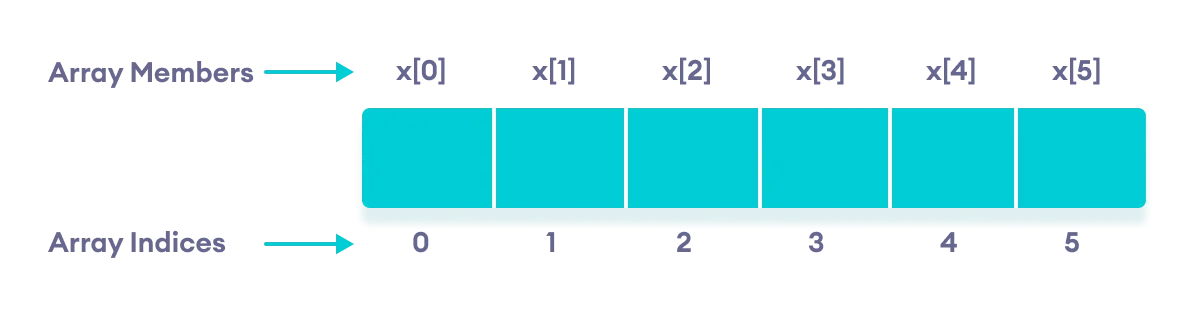
\includegraphics[width=0.8\textwidth]{./assets/images/cpp-array-declaration_0.png}
    \caption{Elements of an array in C++}
    \floatfoot{Elements of an array in C++ from Programiz}
    \label{fig:array-elements}
\end{figure}

Figure \ref{fig:array-elements} shows the the visual representation of the
elements of an array in C++. It shows the array members and indices.

% Code example for array declaration
\begin{lstlisting}[language=C++, caption={Array Declaration}]
// array.cpp
int main() {
    int arr[6];
    return 0;
}
\end{lstlisting}

The above code snippet declares an array named \texttt{arr} of size 6 that
can store 6 integer values. The elements of the array are accessed using
index values from 0 to 5 as shown in Figure \ref{fig:array-elements}.

% Code for assigning values to array elements
\begin{lstlisting}[language=C++, caption={Assigning Values to Array Elements}]
// array_assign.cpp
int main() {
    int arr[6];
    arr[0] = 19;
    arr[1] = 10;
    arr[2] = 8;
    return 0;
}
\end{lstlisting}

The above code snippet assigns values to the elements of the array \texttt{arr}
at index 0, 1, and 2. The elements of the array can be accessed and modified
using their index values. Array elements that are not explicitly initialized
are assigned default values based on their data type. For example, integer
elements are initialized to 0.

% Insert image for array initialization
\begin{figure}[h]
  \centering
  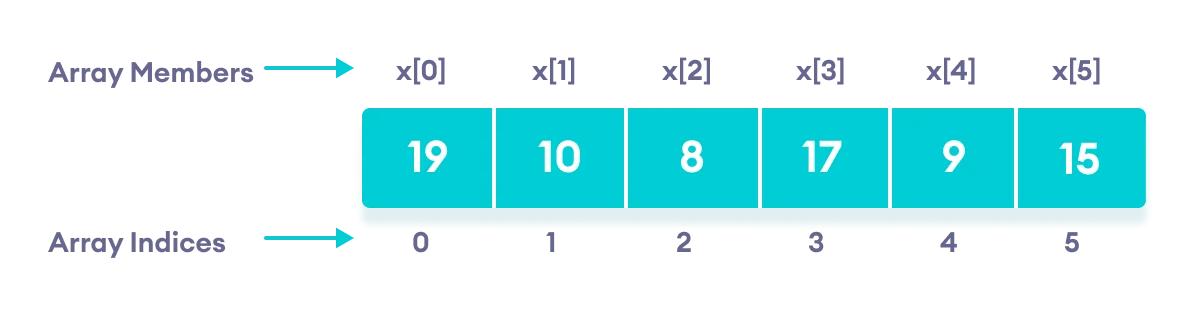
\includegraphics[width=0.8\textwidth]{./assets/images/cpp-array-initialization_0.png}
  \caption{Initializing Array Elements}
    \floatfoot{Initializing Array Elements from Programiz}
    \label{fig:array-initialization}
\end{figure}

Figure \ref{fig:array-initialization} shows the code for initializing array
elements in C++. The array elements are initialized using curly braces
\texttt{\{\}} with the values separated by commas. When the size of the array
is specified, the number of elements in the initialization list must match
the size of the array. If the size of the array is not specified, the size
is automatically determined based on the number of elements in the array
during initialization.

% Code for initializing array elements
\begin{lstlisting}[language=C++, caption={Initializing Array Elements}]
int main() {
    int arr[6] = {19, 10, 8, 17, 9, 15};
    return 0;
}
\end{lstlisting}

The above code snippet initializes the elements of the array \texttt{arr} with
the values 19, 10, 8, 17, 9, and 15. The size of the array is specified as 6,
and the number of elements in the initialization list matches the size of the
array.

% Another code example for array initialization with unspecified size
\begin{lstlisting}[language=C++, caption={Initializing Array Elements with Unspecified Size}]
int main() {
    int arr[] = {19, 10, 8, 17, 9, 15};
    return 0;
}
\end{lstlisting}

The above code snippet initializes the elements of the array \texttt{arr} with
the values 19, 10, 8, 17, 9, and 15. The size of the array is not specified
and is automatically determined based on the number of elements in the
initialization list.

% Figure for array initialization with empty members
\begin{figure}[h]
  \centering
  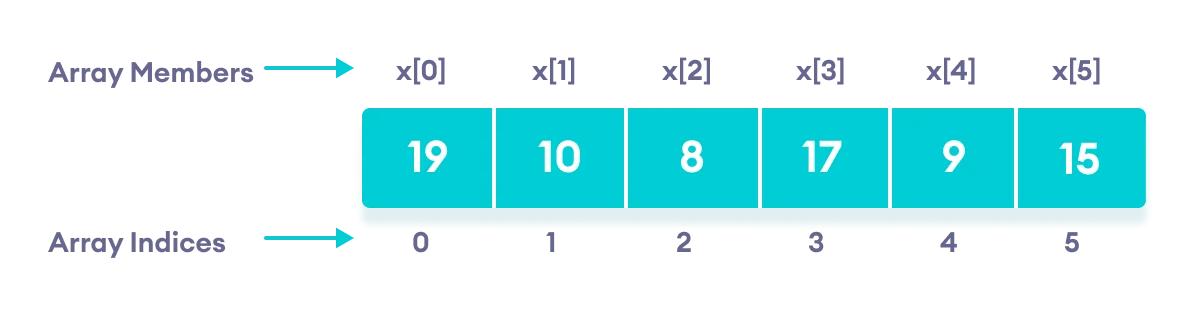
\includegraphics[width=0.8\textwidth]{./assets/images/cpp-array-initialization_0.png}
  \caption{Initializing Array Elements with Empty Members}
    \floatfoot{Initializing Array Elements with Empty Members from Programiz}
    \label{fig:array-initialization-empty}
\end{figure}

Figure \ref{fig:array-initialization-empty} shows the code for initializing
array elements with empty members in C++. The array elements are initialized
using curly braces \texttt{\{\}} with empty members. Empty members only
appear at the end of the initialization list and are assigned default values
based on their data type. For example, integer elements are initialized to 0.

% Code for initializing array elements with empty members
\begin{lstlisting}[language=C++, caption={Initializing Array Elements with Empty Members}]
int main() {
    int arr[6] = {19, 10, 8};
    return 0;
}
\end{lstlisting}

The above code snippet initializes the first three elements of the array
\texttt{arr} with the values 19, 10, and 8. The remaining elements of the
array are initialized to 0, which is the default value for integer elements.

\subsection{Types of Arrays}

There are two main types of arrays in C++: one-dimensional arrays and
multi-dimensional arrays.

\subsubsection{One-dimensional Array}

A \textbf{\textit{one-dimensional array}} is a collection of elements of the
same data type that are stored in a single row. It is the most common type
of array used in computer programming. The elements of a one-dimensional array
are accessed using a single index value.

% Figure for one-dimensional array
\begin{figure}[h]
  \centering
  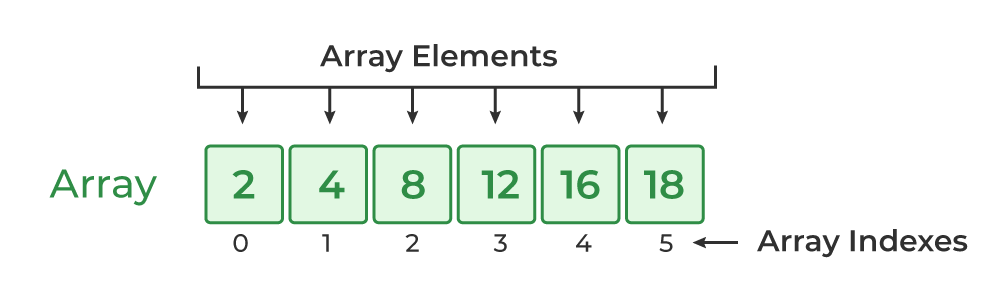
\includegraphics[width=0.8\textwidth]{./assets/images/Arrays-in-C.png}
  \caption{One-dimensional Array in C++}
    \floatfoot{One-dimensional Array in C++ from GeekforGeeks}
    \label{fig:one-dimensional-array}
\end{figure} 

Figure \ref{fig:one-dimensional-array} shows the visual representation of a
one-dimensional array in C++. As shown in the figure, the elements of the
array are stored in a single row, and each element is accessed using a single
index value.

% Code example for one-dimensional array
\begin{lstlisting}[language=C++, caption={One-dimensional Array}]
int main() {
    int arr[6] = {2, 4, 8, 12, 16, 18};
    return 0;
}
\end{lstlisting}

The above code snippet declares and initializes a one-dimensional array named
\texttt{arr} with 6 integer elements. A one-dimensional array only has one
set of square brackets \texttt{[]}. One set of square brackets signifies that
the array is one-dimensional.

\subsubsection{Multi-dimensional Array}

A \textbf{\textit{multi-dimensional array}} is a collection of elements of the
same data type that are stored in multiple rows and columns. It is used to
store data in a tabular format. The elements of a multi-dimensional array are
accessed using multiple index values.

% Figure for two-dimensional array
\begin{figure}[h]
  \centering
  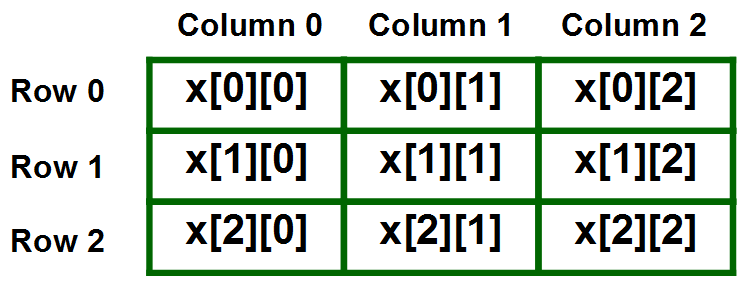
\includegraphics[width=0.8\textwidth]{./assets/images/two-d.png}
  \caption{Two-dimensional Array in C++}
    \floatfoot{Two-dimensional Array in C++ from GeekforGeeks}
    \label{fig:two-dimensional-array}
\end{figure}

Figure \ref{fig:two-dimensional-array} shows the visual representation of a
two-dimensional array in C++. As shown in the figure, the elements of the
array are stored in multiple rows and columns, and each element is accessed
using two index values. The number of elements in a two-dimensional array is
determined by the number of rows and columns.

% Code example for two-dimensional array
\begin{lstlisting}[language=C++, caption={Two-dimensional Array}]
int main() {
    int arr[3][4] = {
        {1, 2, 3, 4},
        {5, 6, 7, 8},
        {9, 10, 11, 12}
    };
    return 0;
}
\end{lstlisting}

The above code snippet declares and initializes a two-dimensional array named
\texttt{arr} with 3 rows and 3 columns. A two-dimensional array has two sets
of square brackets \texttt{[][]}. Two sets of square brackets signify that the
array is two-dimensional. The number of rows and columns in a two-dimensional
array is specified within the square brackets. The first set of square brackets
specifies the number of rows, and the second set of square brackets specifies
the number of columns. Thus, in the above example, the array \texttt{arr} has
3 rows and 4 columns.

% Code With empty members
\begin{lstlisting}[language=C++, caption={Two-dimensional Array with Empty Members}]
int main() {
    int arr[3][4] = {
        {1, 2},
        {5, 6, 7},
        {9}
    };
    return 0;
}
\end{lstlisting}

The above code snippet initializes the elements of the two-dimensional array
\texttt{arr} with empty members. The first row of the array has 2 elements,
the second row has 3 elements, and the third row has 1 element. The remaining
elements of the array are initialized to 0, which is the default value for
integer elements.

\subsection{Array Operations}

Arrays support various operations such as insertion, deletion, and searching
of elements. These operations are essential for manipulating the elements of
an array and performing various tasks in a computer program.

\subsubsection{Insertion}

The \textbf{\textit{insertion}} operation is used to add an element to an array
at a specific position. The element is inserted at the specified index, and
the existing elements are shifted to accommodate the new element.

% TikZ diagram for array insertion
\begin{figure}[h]
    \centering
    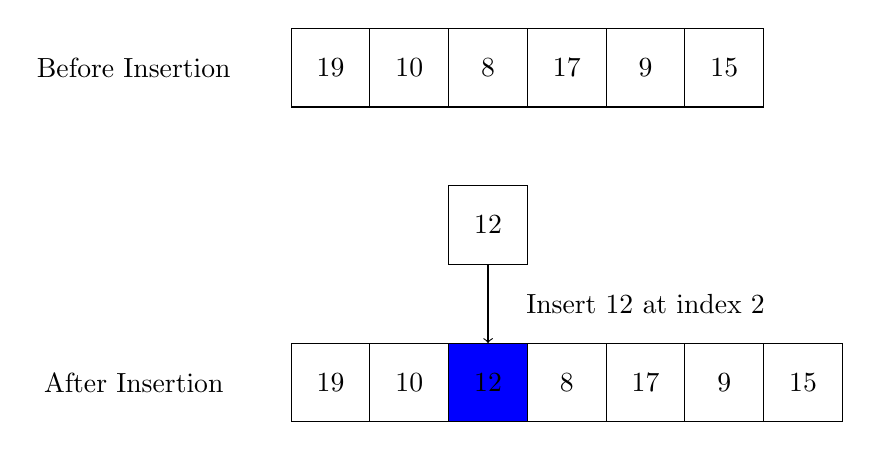
\begin{tikzpicture}
        % Make a one dimensional grid with 6 elements
        \draw (0, 0) grid (6, 1);
        % Fill the grid with the elements
        \foreach \x/\y in {
            0/19, 1/10, 2/8, 3/17, 4/9, 5/15
        }
        \node at (\x + 0.5, 0.5) {\y};
        \node at (-2, 0.5) {Before Insertion};

        % Insert a new element at index 2
        \draw (2, -1) rectangle (3, -2);
        \node at (2.5, -1.5) {12};

        % Draw Arrow with label "Insert"
        \draw[->] (2.5, -2) -- (2.5, -3);
        \node at (4.5, -2.5) {Insert 12 at index 2};
        
        % Create a new grid with the inserted element
        \draw (0, -4) grid (7, -3);
        % Color the grid with inserted element
        \draw[fill=blue] (2, -4) rectangle (3, -3);

        \foreach \x/\y in {
            0/19, 1/10, 2/12, 3/8, 4/17, 5/9, 6/15
        }
        \node at (\x + 0.5, -3.5) {\y};
        \node at (-2, -3.5) {After Insertion};
    \end{tikzpicture}
    \caption{Array Insertion}
    \label{fig:array-insertion}
\end{figure}

Figure \ref{fig:array-insertion} shows the visual representation of the
insertion operation in an array. The element 12 is inserted at index 2 of
the array, and the existing elements are shifted to accommodate the new
element.

% Code example for array insertion
\begin{lstlisting}[language=C++, caption={Array Insertion}, label={lst:array-insertion}]
int main() {
    int arr[100] = {19, 10, 8, 17, 9, 15};
    int n = 6;
    int index = 2;
    int value = 12;

    for (int i = n - 1; i >= index; i--) {
        arr[i + 1] = arr[i];
    }
    arr[index] = value;
    n++;

    return 0;
}
\end{lstlisting}

Code \ref{lst:array-insertion} shows the code for inserting an element
into an array in C++. The code snippet declares an array \texttt{arr} of size
100 and initializes it with 6 elements. It then inserts the element 12 at
index 2 of the array and shifts the existing elements to accommodate the new
element.

\subsubsection{Deletion}

The \textbf{\textit{deletion}} operation is used to remove an element from an
array at a specific position. The element is deleted from the specified index,
and the remaining elements are shifted to fill the gap created by the deletion.

% TikZ diagram for array deletion
\begin{figure}[h]
    \centering
    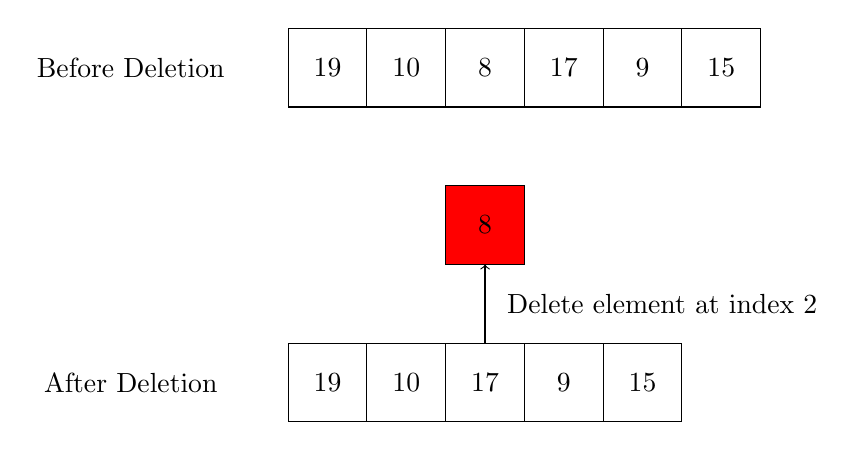
\begin{tikzpicture}
        % Make a one dimensional grid with 6 elements
        \draw (0, 0) grid (6, 1);
        % Fill the grid with the elements
        \foreach \x/\y in {
            0/19, 1/10, 2/8, 3/17, 4/9, 5/15
        }
        \node at (\x + 0.5, 0.5) {\y};
        \node at (-2, 0.5) {Before Deletion};

        % Delete the element at index 2
        \draw[fill=red] (2, -1) rectangle (3, -2);
        \node at (2.5, -1.5) {8};

        % Draw Arrow with label "Delete"
        \draw[->] (2.5, -3) -- (2.5, -2);
        \node at (4.75, -2.5) {Delete element at index 2};
        
        % Create a new grid with the deleted element
        \draw (0, -4) grid (5, -3);

        \foreach \x/\y in {
            0/19, 1/10, 2/17, 3/9, 4/15
        }
        \node at (\x + 0.5, -3.5) {\y};
        \node at (-2, -3.5) {After Deletion};
    \end{tikzpicture}
    \caption{Array Deletion}
    \label{fig:array-deletion}
\end{figure}


Figure \ref{fig:array-deletion} shows the visual representation of the deletion
operation in an array. The element 8 is deleted from index 2 of the array, and
the remaining elements are shifted to fill the gap created by the deletion.

% Code example for array deletion
\begin{lstlisting}[language=C++, caption={Array Deletion}, label={lst:array-deletion}]
int main() {
    int arr[100] = {19, 10, 8, 17, 9, 15};
    int n = 6;
    int index = 2;

    for (int i = index; i < n - 1; i++) {
        arr[i] = arr[i + 1];
    }
    n--;

    return 0;
}
\end{lstlisting}

Code \ref{lst:array-deletion} shows the code for deleting an element from an
array in C++. The code snippet declares an array \texttt{arr} of size 100 and
initializes it with 6 elements. It then deletes the element at index 2 of the
array and shifts the remaining elements to fill the gap created by the deletion.

\subsubsection{Searching}

The \textbf{\textit{searching}} operation is used to find the position of an
element in an array. The element is searched for in the array, and the index
of the element is returned if it is found. If the element is not found, a
special value such as -1 is returned to indicate that the element is not
present in the array.

% TikZ diagram for array searching
\begin{figure}[h]
    \centering
    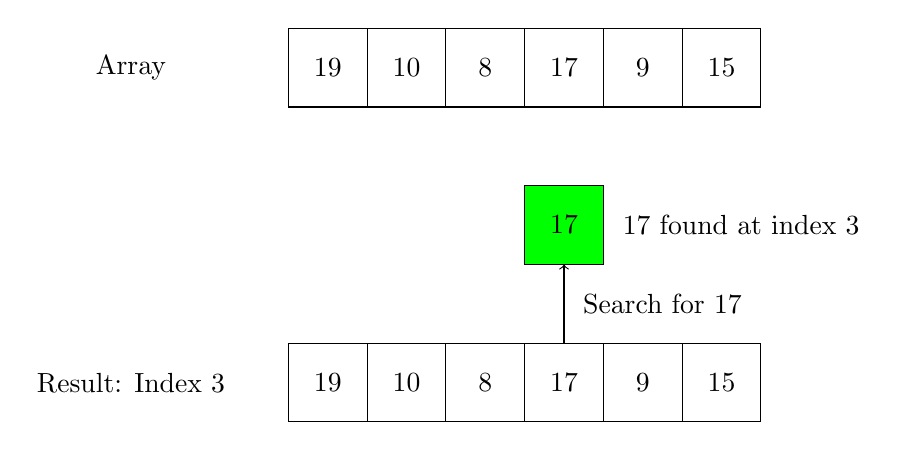
\begin{tikzpicture}
        % Make a one dimensional grid with 6 elements
        \draw (0, 0) grid (6, 1);
        % Fill the grid with the elements
        \foreach \x/\y in {
            0/19, 1/10, 2/8, 3/17, 4/9, 5/15
        }
        \node at (\x + 0.5, 0.5) {\y};
        \node at (-2, 0.5) {Array};

        % Search for the element 17
        \draw[fill=green] (3, -1) rectangle (4, -2);
        \node at (3.5, -1.5) {17};

        % Draw Arrow with label "Search"
        \draw[->] (3.5, -3) -- (3.5, -2);
        \node at (4.75, -2.5) {Search for 17};
        \node at (5.75, -1.5) {17 found at index 3};

        % Create a new grid with the searched element
        \draw (0, -4) grid (6, -3);

        \foreach \x/\y in {
            0/19, 1/10, 2/8, 3/17, 4/9, 5/15
        }
        \node at (\x + 0.5, -3.5) {\y};
        \node at (-2, -3.5) {Result: Index 3};
    \end{tikzpicture}
    \caption{Array Searching}
    \label{fig:array-searching}
\end{figure}

Figure \ref{fig:array-searching} shows the visual representation of the
searching operation in an array. The element 17 is searched for in the array,
and the index of the element is returned if it is found. In this case, the
element 17 is found at index 3 of the array.

% Code example for array searching
\begin{lstlisting}[language=C++, caption={Array Searching}, label={lst:array-searching}]
int main() {
    int arr[100] = {19, 10, 8, 17, 9, 15};
    int n = 6;
    int value = 17;
    int index = -1;

    for (int i = 0; i < n; i++) {
        if (arr[i] == value) {
            index = i;
            break;
        }
    }

    return 0;
}
\end{lstlisting}

Code \ref{lst:array-searching} shows the code for searching an element in an
array in C++. The code snippet declares an array \texttt{arr} of size 100 and
initializes it with 6 elements. It then searches for the element 17 in the
array and returns the index of the element if it is found. In this case, the
element 17 is found at index 3 of the array. The searching algorithm used in
the example is a linear search algorithm.

% \subsection{Complexity Analysis of Arrays}

\section{Linked Lists}

A \textbf{\textit{linked list}} is a data structure that consists of a sequence
of elements called nodes. A node contains a data part and a reference part that
points to the next or previous node in the sequence. Linked lists are used to
store and manipulate collections of elements in a computer program. Unlike
arrays, linked lists do not require contiguous memory locations, and the size
of a linked list can grow or shrink dynamically.

\subsection{Types of Linked Lists}

\subsubsection{Singly Linked List}

A \textbf{\textit{singly linked list}} is a type of linked list in which each
node contains a data part and a next part that points to the next node in the
sequence. The last node in the list points to a special value called NULL to
indicate the end of the list.

% TikZ diagram for singly linked list
\begin{figure}[h]
    \centering
    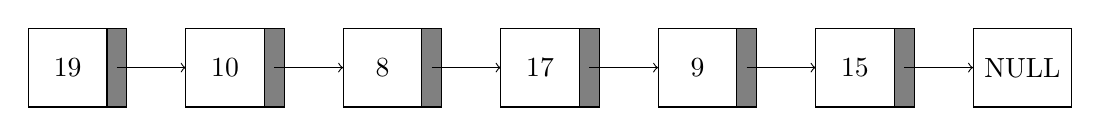
\begin{tikzpicture}
        % Draw the nodes of the singly linked list
        \draw (0, 0) rectangle (1, 1);
        \node at (0.5, 0.5) {19};
        \draw[fill=gray] (1, 1) rectangle (1.25, 0);

        \draw (2, 0) rectangle (3, 1);
        \node at (2.5, 0.5) {10};
        \draw[fill=gray] (3, 1) rectangle (3.25, 0);

        \draw (4, 0) rectangle (5, 1);
        \node at (4.5, 0.5) {8};
        \draw[fill=gray] (5, 1) rectangle (5.25, 0);

        \draw (6, 0) rectangle (7, 1);
        \node at (6.5, 0.5) {17};
        \draw[fill=gray] (7, 1) rectangle (7.25, 0);

        \draw (8, 0) rectangle (9, 1);
        \node at (8.5, 0.5) {9};
        \draw[fill=gray] (9, 1) rectangle (9.25, 0);

        \draw (10, 0) rectangle (11, 1);
        \node at (10.5, 0.5) {15};
        \draw[fill=gray] (11, 1) rectangle (11.25, 0);

        \draw (12, 0) rectangle (13.25, 1);
        \node at (12.625, 0.5) {NULL};

        % Draw the arrows between the nodes
        \draw[->] (1.125, 0.5) -- (2, 0.5);
        \draw[->] (3.125, 0.5) -- (4, 0.5);
        \draw[->] (5.125, 0.5) -- (6, 0.5);
        \draw[->] (7.125, 0.5) -- (8, 0.5);
        \draw[->] (9.125, 0.5) -- (10, 0.5);
        \draw[->] (11.125, 0.5) -- (12, 0.5);
    \end{tikzpicture}
    \caption{Singly Linked List}
    \label{fig:singly-linked-list}
\end{figure}

Figure \ref{fig:singly-linked-list} shows the visual representation of a singly
linked list. The linked list contains nodes with data values 19, 10, 8, 17, 9,
and 15. Each node points to the next node in the sequence, and the last node
points to NULL to indicate the end of the list.

% Code example for singly linked list
\begin{lstlisting}[language=C++, caption={Singly Linked List}, label={lst:singly-linked-list}]
struct Node {
    int data;
    Node *next;
    
    Node(int data) {
        this->data = data;
        this->next = NULL;
    }
};

int main() {
    Node *first = new Node(19);
    Node *second = new Node(10);
    Node *third = new Node(8);
    Node *fourth = new Node(17);
    Node *fifth = new Node(9);
    Node *sixth = new Node(15);

    Node *head = first;

    first->next = second;
    second->next = third;
    third->next = fourth;
    fourth->next = fifth;
    fifth->next = sixth;

    return 0;
}
\end{lstlisting}

Code \ref{lst:singly-linked-list} shows the code for creating a singly linked
list in C++. The code snippet defines a structure \texttt{Node} that contains
a data part and a next part that points to the next node in the sequence. It
then creates a linked list with nodes containing data values 19, 10, 8, 17, 9,
and 15. Each node points to the next node in the sequence, and the last node
points to NULL to indicate the end of the list.

\subsubsection{Doubly Linked List}

A \textbf{\textit{doubly linked list}} is a type of linked list in which each
node contains a data part, a next part that points to the next node in the
sequence, and a previous part that points to the previous node in the sequence.
The first node in the list points to NULL in the previous part, and the last
node in the list points to NULL in the next part.

% TikZ diagram for doubly linked list
\begin{figure}[h]
    \centering
    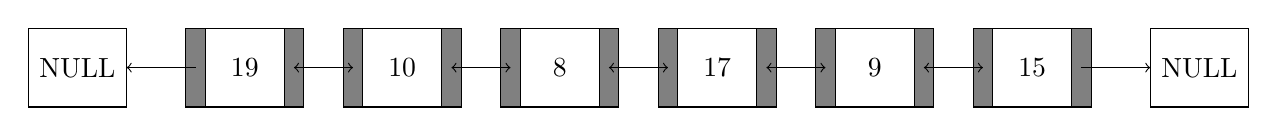
\begin{tikzpicture}
        % Draw the nodes of the doubly linked list
        \draw (-1, 0) rectangle (-2.25, 1);
        \node at (-1.625, 0.5) {NULL};

        \draw (0, 0) rectangle (1, 1);
        \node at (0.5, 0.5) {19};
        \draw[fill=gray] (1, 1) rectangle (1.25, 0);
        \draw[fill=gray] (-0.25, 1) rectangle (0, 0);

        \draw (2, 0) rectangle (3, 1);
        \node at (2.5, 0.5) {10};
        \draw[fill=gray] (3, 1) rectangle (3.25, 0);
        \draw[fill=gray] (1.75, 1) rectangle (2, 0);

        \draw (4, 0) rectangle (5, 1);
        \node at (4.5, 0.5) {8};
        \draw[fill=gray] (5, 1) rectangle (5.25, 0);
        \draw[fill=gray] (3.75, 1) rectangle (4, 0);

        \draw (6, 0) rectangle (7, 1);
        \node at (6.5, 0.5) {17};
        \draw[fill=gray] (7, 1) rectangle (7.25, 0);
        \draw[fill=gray] (5.75, 1) rectangle (6, 0);

        \draw (8, 0) rectangle (9, 1);
        \node at (8.5, 0.5) {9};
        \draw[fill=gray] (9, 1) rectangle (9.25, 0);
        \draw[fill=gray] (7.75, 1) rectangle (8, 0);

        \draw (10, 0) rectangle (11, 1);
        \node at (10.5, 0.5) {15};
        \draw[fill=gray] (11, 1) rectangle (11.25, 0);
        \draw[fill=gray] (9.75, 1) rectangle (10, 0);

        \draw (12, 0) rectangle (13.25, 1);
        \node at (12.625, 0.5) {NULL};

        % Draw the arrows between the nodes
        \draw[<-] (-1, 0.5) -- (-0.125, 0.5);
        \draw[<->] (1.125, 0.5) -- (1.875, 0.5);
        \draw[<->] (3.125, 0.5) -- (3.875, 0.5);
        \draw[<->] (5.125, 0.5) -- (5.875, 0.5);
        \draw[<->] (7.125, 0.5) -- (7.875, 0.5);
        \draw[<->] (9.125, 0.5) -- (9.875, 0.5);
        \draw[->] (11.125, 0.5) -- (12, 0.5);
    \end{tikzpicture}
    \caption{Doubly Linked List}
    \label{fig:doubly-linked-list}
\end{figure}

Figure \ref{fig:doubly-linked-list} shows the visual representation of a doubly
linked list. The linked list contains nodes with data values 19, 10, 8, 17, 9,
and 15. Each node points to the next and previous nodes in the sequence, and
the first and last nodes point to NULL to indicate the end of the list.

% Code example for doubly linked list
\begin{lstlisting}[language=C++, caption={Doubly Linked List}, label={lst:doubly-linked-list}]
struct Node {
    int data;
    Node *next;
    Node *prev;
    
    Node(int data) {
        this->data = data;
        this->next = NULL;
        this->prev = NULL;
    }
};

int main() {
    Node *first = new Node(19);
    Node *second = new Node(10);
    Node *third = new Node(8);
    Node *fourth = new Node(17);
    Node *fifth = new Node(9);
    Node *sixth = new Node(15);

    Node *head = first;

    first->next = second;
    second->next = third;
    third->next = fourth;
    fourth->next = fifth;
    fifth->next = sixth;
    
    second->prev = first;
    third->prev = second;
    fourth->prev = third;
    fifth->prev = fourth;
    sixth->prev = fifth;

    return 0;
}
\end{lstlisting}

Code \ref{lst:doubly-linked-list} shows the code for creating a doubly linked
list in C++. The code snippet defines a structure \texttt{Node} that contains
a data part, a next part that points to the next node in the sequence, and a
previous part that points to the previous node in the sequence. It then creates
a linked list with nodes containing data values 19, 10, 8, 17, 9, and 15. Each
node points to the next and previous nodes in the sequence, and the first and
last nodes point to NULL to indicate the end of the list.

\subsubsection{Circular Linked List}

A \textbf{\textit{circular linked list}} is a type of linked list in which the
last node in the list points back to the first node, forming a circular loop.
This allows traversal of the list in a circular manner, starting from any node
in the list.

% TikZ diagram for circular linked list
\begin{figure}[h]
    \centering
    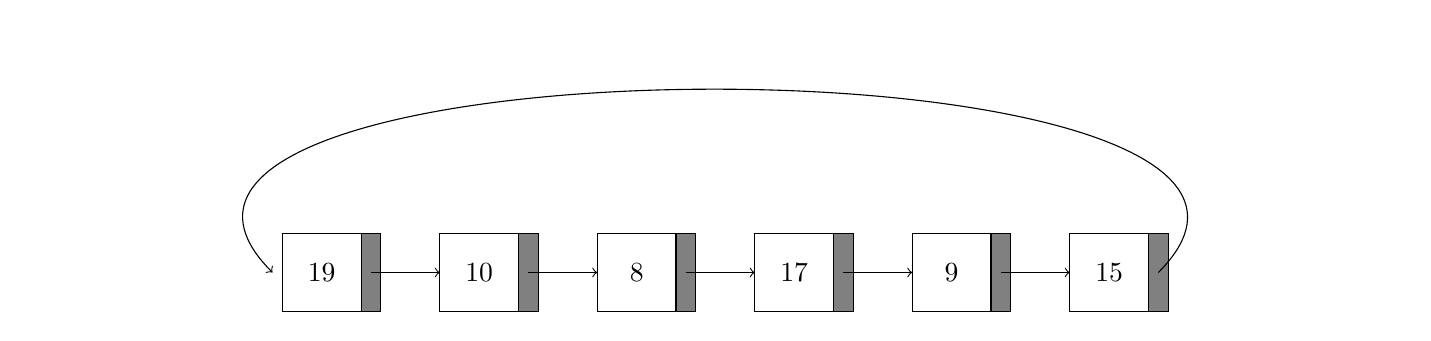
\begin{tikzpicture}
        % Draw the nodes of the circular linked list
        \draw (0, 0) rectangle (1, 1);
        \node at (0.5, 0.5) {19};
        \draw[fill=gray] (1, 1) rectangle (1.25, 0);

        \draw (2, 0) rectangle (3, 1);
        \node at (2.5, 0.5) {10};
        \draw[fill=gray] (3, 1) rectangle (3.25, 0);

        \draw (4, 0) rectangle (5, 1);
        \node at (4.5, 0.5) {8};
        \draw[fill=gray] (5, 1) rectangle (5.25, 0);

        \draw (6, 0) rectangle (7, 1);
        \node at (6.5, 0.5) {17};
        \draw[fill=gray] (7, 1) rectangle (7.25, 0);

        \draw (8, 0) rectangle (9, 1);
        \node at (8.5, 0.5) {9};
        \draw[fill=gray] (9, 1) rectangle (9.25, 0);

        \draw (10, 0) rectangle (11, 1);
        \node at (10.5, 0.5) {15};
        \draw[fill=gray] (11, 1) rectangle (11.25, 0);

        % Draw the arrows between the nodes
        \draw[->] (1.125, 0.5) -- (2, 0.5);
        \draw[->] (3.125, 0.5) -- (4, 0.5);
        \draw[->] (5.125, 0.5) -- (6, 0.5);
        \draw[->] (7.125, 0.5) -- (8, 0.5);
        \draw[->] (9.125, 0.5) -- (10, 0.5);

        % Add Curved Arrow from last node to first node
        \draw[->] (11.125, 0.5) to [out=45, in=135] (-0.125, 0.5);
    \end{tikzpicture}
    \caption{Circular Linked List}
    \label{fig:circular-linked-list}
\end{figure}

Figure \ref{fig:circular-linked-list} shows the visual representation of a
circular linked list. The linked list contains nodes with data values 19, 10,
8, 17, 9, and 15. Each node points to the next node in the sequence, and the
last node points back to the first node, forming a circular loop.

% Code example for circular linked list
\begin{lstlisting}[language=C++, caption={Circular Linked List}, label={lst:circular-linked-list}]
struct Node {
    int data;
    Node *next;
    
    Node(int data) {
        this->data = data;
        this->next = NULL;
    }
};

int main() {
    Node *first = new Node(19);
    Node *second = new Node(10);
    Node *third = new Node(8);
    Node *fourth = new Node(17);
    Node *fifth = new Node(9);
    Node *sixth = new Node(15);

    Node *head = first;

    first->next = second;
    second->next = third;
    third->next = fourth;
    fourth->next = fifth;
    fifth->next = sixth;
    sixth->next = head;

    return 0;
}
\end{lstlisting}

Code \ref{lst:circular-linked-list} shows the code for creating a circular
linked list in C++. The code snippet defines a structure \texttt{Node} that
contains a data part and a next part that points to the next node in the
sequence. It then creates a linked list with nodes containing data values 19,
10, 8, 17, 9, and 15. Each node points to the next node in the sequence, and
the last node points back to the first node, forming a circular loop.

\subsubsection{Doubly Circular Linked List}

A \textbf{\textit{doubly circular linked list}} is a type of linked list in
which each node contains a data part, a next part that points to the next node
in the sequence, and a previous part that points to the previous node in the
sequence. The first node in the list points to the last node in the previous
part, and the last node in the list points to the first node in the next part,
forming a circular loop.

% TikZ diagram for doubly circular linked list
\begin{figure}[h]
    \centering
    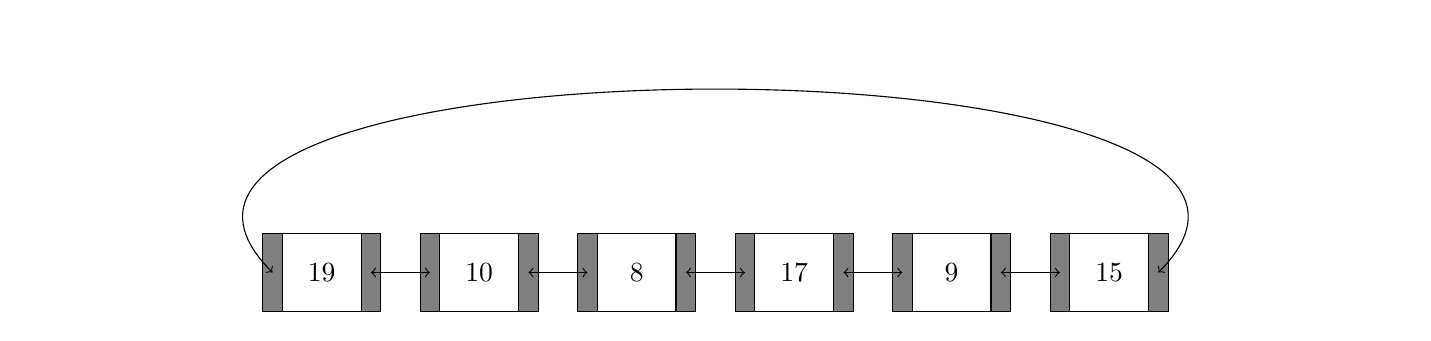
\begin{tikzpicture}
        % Draw the nodes of the doubly circular linked list
        \draw (0, 0) rectangle (1, 1);
        \node at (0.5, 0.5) {19};
        \draw[fill=gray] (1, 1) rectangle (1.25, 0);
        \draw[fill=gray] (-0.25, 1) rectangle (0, 0);

        \draw (2, 0) rectangle (3, 1);
        \node at (2.5, 0.5) {10};
        \draw[fill=gray] (3, 1) rectangle (3.25, 0);
        \draw[fill=gray] (1.75, 1) rectangle (2, 0);

        \draw (4, 0) rectangle (5, 1);
        \node at (4.5, 0.5) {8};
        \draw[fill=gray] (5, 1) rectangle (5.25, 0);
        \draw[fill=gray] (3.75, 1) rectangle (4, 0);

        \draw (6, 0) rectangle (7, 1);
        \node at (6.5, 0.5) {17};
        \draw[fill=gray] (7, 1) rectangle (7.25, 0);
        \draw[fill=gray] (5.75, 1) rectangle (6, 0);

        \draw (8, 0) rectangle (9, 1);
        \node at (8.5, 0.5) {9};
        \draw[fill=gray] (9, 1) rectangle (9.25, 0);
        \draw[fill=gray] (7.75, 1) rectangle (8, 0);

        \draw (10, 0) rectangle (11, 1);
        \node at (10.5, 0.5) {15};
        \draw[fill=gray] (11, 1) rectangle (11.25, 0);
        \draw[fill=gray] (9.75, 1) rectangle (10, 0);

        % Draw the arrows between the nodes
        \draw[<->] (1.125, 0.5) -- (1.875, 0.5);
        \draw[<->] (3.125, 0.5) -- (3.875, 0.5);
        \draw[<->] (5.125, 0.5) -- (5.875, 0.5);
        \draw[<->] (7.125, 0.5) -- (7.875, 0.5);
        \draw[<->] (9.125, 0.5) -- (9.875, 0.5);
        
        % Add Curved Arrow from last node to first node
        \draw[<->] (11.125, 0.5) to [out=45, in=135] (-0.125, 0.5);
    \end{tikzpicture}
    \caption{Doubly Circular Linked List}
    \label{fig:doubly-circular-linked-list}
\end{figure}

Figure \ref{fig:doubly-circular-linked-list} shows the visual representation of
a doubly circular linked list. The linked list contains nodes with data values
19, 10, 8, 17, 9, and 15. Each node points to the next and previous nodes in
the sequence, and the first and last nodes point to each other, forming a
circular loop.

% Code example for doubly circular linked list
\begin{lstlisting}[language=C++, caption={Doubly Circular Linked List}, label={lst:doubly-circular-linked-list}]
struct Node {
    int data;
    Node *next;
    Node *prev;
    
    Node(int data) {
        this->data = data;
        this->next = NULL;
        this->prev = NULL;
    }
};

int main() {
    Node *first = new Node(19);
    Node *second = new Node(10);
    Node *third = new Node(8);
    Node *fourth = new Node(17);
    Node *fifth = new Node(9);
    Node *sixth = new Node(15);

    Node *head = first;

    first->next = second;
    second->next = third;
    third->next = fourth;
    fourth->next = fifth;
    fifth->next = sixth;
    sixth->next = first;

    first->prev = sixth;
    second->prev = first;
    third->prev = second;
    fourth->prev = third;
    fifth->prev = fourth;
    sixth->prev = fifth;

    return 0;
}
\end{lstlisting}

Code \ref{lst:doubly-circular-linked-list} shows the code for creating a doubly
circular linked list in C++. The code snippet defines a structure \texttt{Node}
that contains a data part, a next part that points to the next node in the
sequence, and a previous part that points to the previous node in the sequence.
It then creates a linked list with nodes containing data values 19, 10, 8, 17,
9, and 15. Each node points to the next and previous nodes in the sequence, and
the first and last nodes point to each other, forming a circular loop.

\subsection{Operations on Linked Lists}

\subsubsection{Insertion}

The \textbf{\textit{insertion}} operation is used to add a new node to a linked
list at a specific position. The new node is inserted at the specified position,
and the existing nodes are adjusted to accommodate the new node.

% TikZ diagram for linked list insertion
\begin{figure}[h]
    \centering
    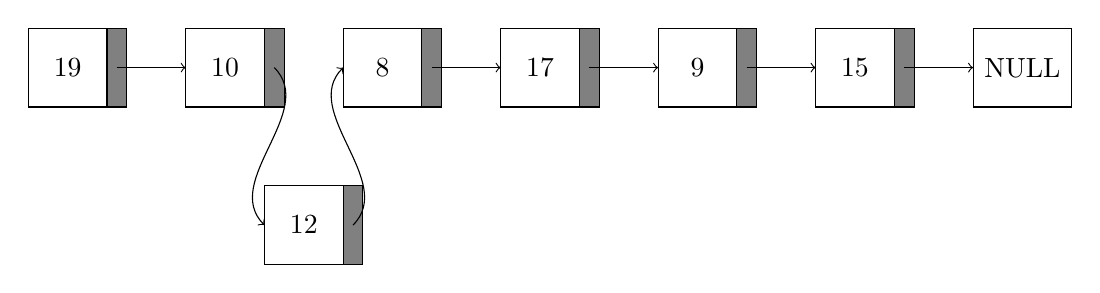
\begin{tikzpicture}
        % Draw the nodes of the linked list
        \draw (0, 0) rectangle (1, 1);
        \node at (0.5, 0.5) {19};
        \draw[fill=gray] (1, 1) rectangle (1.25, 0);

        \draw (2, 0) rectangle (3, 1);
        \node at (2.5, 0.5) {10};
        \draw[fill=gray] (3, 1) rectangle (3.25, 0);

        \draw (4, 0) rectangle (5, 1);
        \node at (4.5, 0.5) {8};
        \draw[fill=gray] (5, 1) rectangle (5.25, 0);

        \draw (6, 0) rectangle (7, 1);
        \node at (6.5, 0.5) {17};
        \draw[fill=gray] (7, 1) rectangle (7.25, 0);

        \draw (8, 0) rectangle (9, 1);
        \node at (8.5, 0.5) {9};
        \draw[fill=gray] (9, 1) rectangle (9.25, 0);

        \draw (10, 0) rectangle (11, 1);
        \node at (10.5, 0.5) {15};
        \draw[fill=gray] (11, 1) rectangle (11.25, 0);

        \draw (12, 0) rectangle (13.25, 1);
        \node at (12.625, 0.5) {NULL};

        % Insert the element 12 at index 2
        \draw (3, -1) rectangle (4, -2);
        \node at (3.5, -1.5) {12};
        \draw[fill=gray] (4, -1) rectangle (4.25, -2);

        % Draw the arrows between the nodes
        \draw[->] (1.125, 0.5) -- (2, 0.5);
        \draw[->] (5.125, 0.5) -- (6, 0.5);
        \draw[->] (7.125, 0.5) -- (8, 0.5);
        \draw[->] (9.125, 0.5) -- (10, 0.5);
        \draw[->] (11.125, 0.5) -- (12, 0.5);

        % Draw curved arrows for the inserted element
        \draw[->] (3.125, 0.5) to [out=315, in=135] (3.0, -1.5);
        \draw[->] (4.125, -1.5) to [out=45, in=225] (4.0, 0.5);
    \end{tikzpicture}
    \caption{Linked List Insertion}
    \label{fig:linked-list-insertion}
\end{figure}

Figure \ref{fig:linked-list-insertion} shows the visual representation of the
insertion operation in a linked list. The element 12 is inserted at index 2 of
the linked list, and the existing nodes are adjusted to accommodate the new
node. 

% Code example for linked list insertion
\begin{lstlisting}[language=C++, caption={Linked List Insertion}, label={lst:linked-list-insertion}]
struct Node {
    int data;
    Node *next;
    
    Node(int data) {
        this->data = data;
        this->next = NULL;
    }
};

int main() {
    Node *first = new Node(19);
    Node *second = new Node(10);
    Node *third = new Node(8);
    Node *fourth = new Node(17);
    Node *fifth = new Node(9);
    Node *sixth = new Node(15);

    Node *head = first;

    first->next = second;
    second->next = third;
    third->next = fourth;
    fourth->next = fifth;
    fifth->next = sixth;

    Node *newNode = new Node(12);
    Node *temp = head;
    int index = 2;

    for (int i = 0; i < index - 1; i++) {
        temp = temp->next;
    }

    newNode->next = temp->next;
    temp->next = newNode;

    return 0;
}
\end{lstlisting}

Code \ref{lst:linked-list-insertion} shows the code for inserting an element in
a linked list in C++. The code snippet defines a structure \texttt{Node} that
contains a data part and a next part that points to the next node in the
sequence. It then creates a linked list with nodes containing data values 19,
10, 8, 17, 9, and 15. The element 12 is inserted at index 2 of the linked list,
and the existing nodes are adjusted to accommodate the new node.

\subsubsection{Deletion}

The \textbf{\textit{deletion}} operation is used to remove a node from a linked
list at a specific position. The node at the specified position is removed, and
the existing nodes are adjusted to maintain the integrity of the list.

% TikZ diagram for linked list deletion
\begin{figure}[h]
    \centering
    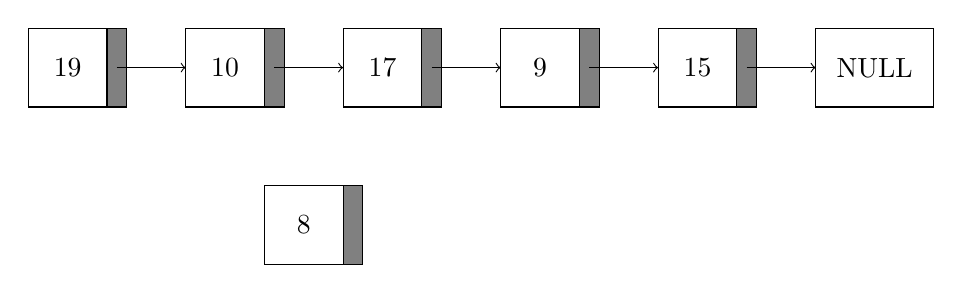
\begin{tikzpicture}
        % Draw the nodes of the linked list
        \draw (0, 0) rectangle (1, 1);
        \node at (0.5, 0.5) {19};
        \draw[fill=gray] (1, 1) rectangle (1.25, 0);

        \draw (2, 0) rectangle (3, 1);
        \node at (2.5, 0.5) {10};
        \draw[fill=gray] (3, 1) rectangle (3.25, 0);

        % \draw (4, 0) rectangle (5, 1);
        % \node at (4.5, 0.5) {8};
        % \draw[fill=gray] (5, 1) rectangle (5.25, 0);

        \draw (4, 0) rectangle (5, 1);
        \node at (4.5, 0.5) {17};
        \draw[fill=gray] (5, 1) rectangle (5.25, 0);

        \draw (6, 0) rectangle (7, 1);
        \node at (6.5, 0.5) {9};
        \draw[fill=gray] (7, 1) rectangle (7.25, 0);

        \draw (8, 0) rectangle (9, 1);
        \node at (8.5, 0.5) {15};
        \draw[fill=gray] (9, 1) rectangle (9.25, 0);

        \draw (10, 0) rectangle (11.5, 1);
        \node at (10.75, 0.5) {NULL};

        % Delete the element at index 2
        \draw (3, -1) rectangle (4, -2);
        \node at (3.5, -1.5) {8};
        \draw[fill=gray] (4, -1) rectangle (4.25, -2);

        % Draw the arrows between the nodes
        \draw[->] (1.125, 0.5) -- (2, 0.5);
        \draw[->] (3.125, 0.5) -- (4, 0.5);
        \draw[->] (5.125, 0.5) -- (6, 0.5);
        \draw[->] (7.125, 0.5) -- (8, 0.5);
        \draw[->] (9.125, 0.5) -- (10, 0.5); 
    \end{tikzpicture}
    \caption{Linked List Deletion}
    \label{fig:linked-list-deletion}
\end{figure}

Figure \ref{fig:linked-list-deletion} shows the visual representation of the
deletion operation in a linked list. The element 10 is deleted from index 2 of
the linked list, and the existing nodes are adjusted to maintain the integrity
of the list.

% Code example for linked list deletion
\begin{lstlisting}[language=C++, caption={Linked List Deletion}, label={lst:linked-list-deletion}]
struct Node {
    int data;
    Node *next;
    
    Node(int data) {
        this->data = data;
        this->next = NULL;
    }
};

int main() {
    Node *first = new Node(19);
    Node *second = new Node(10);
    Node *third = new Node(8);
    Node *fourth = new Node(17);
    Node *fifth = new Node(9);
    Node *sixth = new Node(15);

    Node *head = first;

    first->next = second;
    second->next = third;
    third->next = fourth;
    fourth->next = fifth;
    fifth->next = sixth;

    Node *temp = head;
    int index = 2;

    for (int i = 0; i < index - 1; i++) {
        temp = temp->next;
    }

    Node *deletedNode = temp->next;
    temp->next = temp->next->next;
    delete deletedNode;

    return 0;
}
\end{lstlisting}

Code \ref{lst:linked-list-deletion} shows the code for deleting an element from
a linked list in C++. The code snippet defines a structure \texttt{Node} that
contains a data part and a next part that points to the next node in the
sequence. It then creates a linked list with nodes containing data values 19,
10, 8, 17, 9, and 15. The element 10 is deleted from index 2 of the linked
list, and the existing nodes are adjusted to maintain the integrity of the list.

\subsubsection{Searching}

The \textbf{\textit{searching}} operation is used to find a specific element in
a linked list. The list is traversed from the head node to the last node to find
the element with the specified value.

% TikZ diagram for linked list searching
\begin{figure}[h]
    \centering
    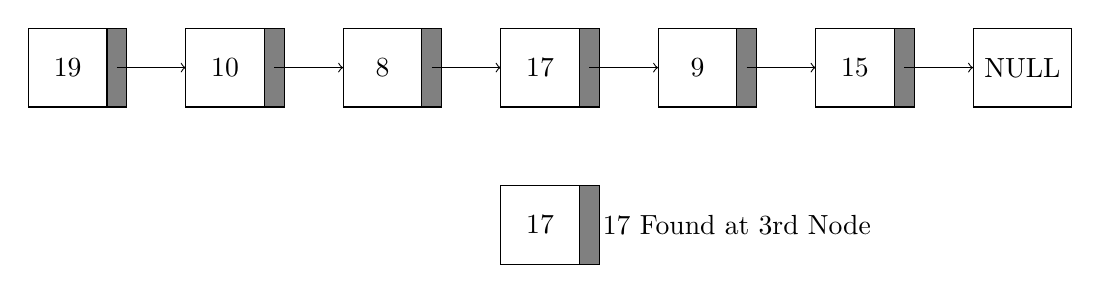
\begin{tikzpicture}
        % Draw the nodes of the linked list
        \draw (0, 0) rectangle (1, 1);
        \node at (0.5, 0.5) {19};
        \draw[fill=gray] (1, 1) rectangle (1.25, 0);

        \draw (2, 0) rectangle (3, 1);
        \node at (2.5, 0.5) {10};
        \draw[fill=gray] (3, 1) rectangle (3.25, 0);

        \draw (4, 0) rectangle (5, 1);
        \node at (4.5, 0.5) {8};
        \draw[fill=gray] (5, 1) rectangle (5.25, 0);

        \draw (6, 0) rectangle (7, 1);
        \node at (6.5, 0.5) {17};
        \draw[fill=gray] (7, 1) rectangle (7.25, 0);

        \draw (8, 0) rectangle (9, 1);
        \node at (8.5, 0.5) {9};
        \draw[fill=gray] (9, 1) rectangle (9.25, 0);

        \draw (10, 0) rectangle (11, 1);
        \node at (10.5, 0.5) {15};
        \draw[fill=gray] (11, 1) rectangle (11.25, 0);

        \draw (12, 0) rectangle (13.25, 1);
        \node at (12.625, 0.5) {NULL};

        % Search for the element 17
        \draw (6, -1) rectangle (7, -2);
        \node at (6.5, -1.5) {17};
        \draw[fill=gray] (7, -1) rectangle (7.25, -2);

        % Label the search result
        \node at (9, -1.5) {17 Found at 3rd Node};

        % Draw the arrows between the nodes
        \draw[->] (1.125, 0.5) -- (2, 0.5);
        \draw[->] (3.125, 0.5) -- (4, 0.5);
        \draw[->] (5.125, 0.5) -- (6, 0.5);
        \draw[->] (7.125, 0.5) -- (8, 0.5);
        \draw[->] (9.125, 0.5) -- (10, 0.5);
        \draw[->] (11.125, 0.5) -- (12, 0.5);
    \end{tikzpicture}
    \caption{Linked List Searching}
    \label{fig:linked-list-searching}
\end{figure}

Figure \ref{fig:linked-list-searching} shows the visual representation of the
searching operation in a linked list. The element 17 is searched for in the
linked list, and the list is traversed from the head node to the last node to
find the element with the specified value.

% Code example for linked list searching
\begin{lstlisting}[language=C++, caption={Linked List Searching}, label={lst:linked-list-searching}]
struct Node {
    int data;
    Node *next;
    
    Node(int data) {
        this->data = data;
        this->next = NULL;
    }
};

int main() {
    Node *first = new Node(19);
    Node *second = new Node(10);
    Node *third = new Node(8);
    Node *fourth = new Node(17);
    Node *fifth = new Node(9);
    Node *sixth = new Node(15);

    Node *head = first;

    first->next = second;
    second->next = third;
    third->next = fourth;
    fourth->next = fifth;
    fifth->next = sixth;

    int searchValue = 17;
    Node *temp = head;
    int index = 0;

    while (temp != NULL) {
        if (temp->data == searchValue) {
            break;
        }
        temp = temp->next;
        index++;
    }

    return 0;
}
\end{lstlisting}
    
Code \ref{lst:linked-list-searching} shows the code for searching an element in
a linked list in C++. The code snippet defines a structure \texttt{Node} that
contains a data part and a next part that points to the next node in the
sequence. It then creates a linked list with nodes containing data values 19,
10, 8, 17, 9, and 15. The element 17 is searched for in the linked list, and
the list is traversed from the head node to the last node to find the element
with the specified value.

% \subsection{Complexity Analysis of Linked Lists}

\section{Comparison of Arrays and Linked Lists}

Unlike arrays, linked lists do not have a fixed size and can grow dynamically
by adding new nodes. This makes linked lists more flexible and efficient for
insertion and deletion operations, as they do not require shifting elements to
accommodate new elements. However, linked lists have higher memory overhead due
to the additional pointers in each node.

Arrays are more efficient for random access operations, as elements can be
accessed directly using their index. In contrast, linked lists require
traversing the list from the head node to the desired node, which can be slower
for large lists. Arrays also have better cache locality, as elements are stored
contiguously in memory, leading to faster access times.

Thus, if the application requires frequent insertion and deletion operations
with a dynamic size, linked lists are a better choice. On the other hand, if the
application requires frequent random access operations and has a fixed size,
arrays are more suitable.

\section{Summary}

In this chapter, we discussed arrays and linked lists as fundamental data
structures in computer science. We covered the basic concepts, operations, and
implementations of arrays and linked lists, along with their comparison in terms
of performance and memory usage. We also explored different types of linked
lists, such as singly linked lists, doubly linked lists, circular linked lists,
and doubly circular linked lists, and discussed the operations on linked lists,
such as insertion, deletion, and searching. Finally, we compared arrays and
linked lists based on their characteristics and use cases.

\section{Coding Exercises}

\begin{enumerate}
    % Reverse an Array
    \item \textbf{Reverse an Array:} Write a C++ program to reverse an array of
    integers. The program should take the size of the array and the elements of
    the array as input and output the reversed array.
    \begin{enumerate}
        \item Declare an array of integers with a fixed size.
        \begin{align*}
            \text{int arr[6];}
        \end{align*}
        \item Initialize the array with the input elements.
        \begin{align*}
            \text{arr = \{19, 10, 8, 17, 9, 15\};}
        \end{align*}
        \item Reverse the array using a loop. \\
        \begin{center}
            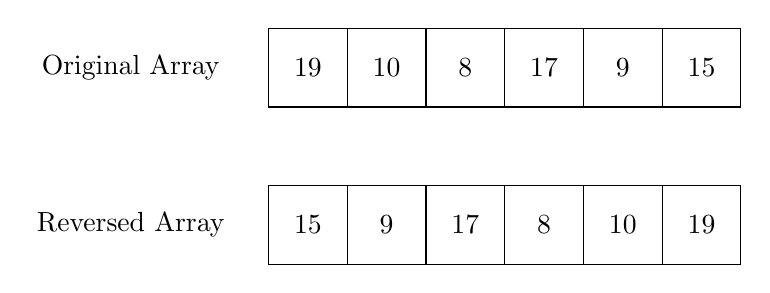
\begin{tikzpicture}[scale=1]
                \draw (0, 0) grid (6, 1);
                \node at (0.5, 0.5) {19};
                \node at (1.5, 0.5) {10};
                \node at (2.5, 0.5) {8};
                \node at (3.5, 0.5) {17};
                \node at (4.5, 0.5) {9};
                \node at (5.5, 0.5) {15};
                \node at (-1.75, 0.5) {Original Array};

                % \draw[->] (3, 0) -- (3, -1);

                \draw (0, -1) grid (6, -2);
                \node at (0.5, -1.5) {15};
                \node at (1.5, -1.5) {9};
                \node at (2.5, -1.5) {17};
                \node at (3.5, -1.5) {8};
                \node at (4.5, -1.5) {10};
                \node at (5.5, -1.5) {19};
                \node at (-1.75, -1.5) {Reversed Array};
            \end{tikzpicture}
        \end{center}
        \item Print the reversed array to the console.
        \begin{align*}
            \text{Reversed Array: 15, 9, 17, 8, 10, 19}
        \end{align*}
        \item Determine the \textbf{time complexity} and
        \textbf{space complexity} of the program.
    \end{enumerate}

    % Reverse a Linked List
    \item \textbf{Reverse a Linked List:} Write a C++ program to reverse a singly
    linked list. The program should take the elements of the linked list as input
    and output the reversed linked list.

    \begin{enumerate}
        \item Create a singly linked list with nodes containing the elements
        \begin{center}
            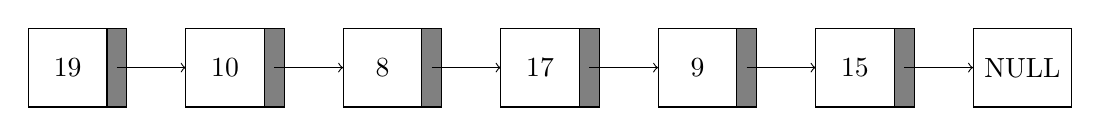
\begin{tikzpicture}
                \draw (0, 0) rectangle (1, 1);
                \node at (0.5, 0.5) {19};
                \draw[fill=gray] (1, 1) rectangle (1.25, 0);
    
                \draw (2, 0) rectangle (3, 1);
                \node at (2.5, 0.5) {10};
                \draw[fill=gray] (3, 1) rectangle (3.25, 0);
    
                \draw (4, 0) rectangle (5, 1);
                \node at (4.5, 0.5) {8};
                \draw[fill=gray] (5, 1) rectangle (5.25, 0);
    
                \draw (6, 0) rectangle (7, 1);
                \node at (6.5, 0.5) {17};
                \draw[fill=gray] (7, 1) rectangle (7.25, 0);
    
                \draw (8, 0) rectangle (9, 1);
                \node at (8.5, 0.5) {9};
                \draw[fill=gray] (9, 1) rectangle (9.25, 0);
    
                \draw (10, 0) rectangle (11, 1);
                \node at (10.5, 0.5) {15};
                \draw[fill=gray] (11, 1) rectangle (11.25, 0);
    
                \draw (12, 0) rectangle (13.25, 1);
                \node at (12.625, 0.5) {NULL};
    
                \draw[->] (1.125, 0.5) -- (2, 0.5);
                \draw[->] (3.125, 0.5) -- (4, 0.5);
                \draw[->] (5.125, 0.5) -- (6, 0.5);
                \draw[->] (7.125, 0.5) -- (8, 0.5);
                \draw[->] (9.125, 0.5) -- (10, 0.5);
                \draw[->] (11.125, 0.5) -- (12, 0.5);
            \end{tikzpicture}
        \end{center}
        \item Reverse the linked list using a loop.
        \begin{center}
            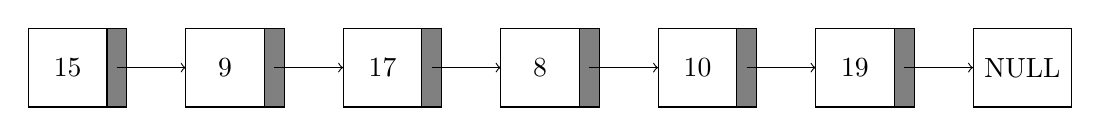
\begin{tikzpicture}
                \draw (0, 0) rectangle (1, 1);
                \node at (0.5, 0.5) {15};
                \draw[fill=gray] (1, 1) rectangle (1.25, 0);
    
                \draw (2, 0) rectangle (3, 1);
                \node at (2.5, 0.5) {9};
                \draw[fill=gray] (3, 1) rectangle (3.25, 0);
    
                \draw (4, 0) rectangle (5, 1);
                \node at (4.5, 0.5) {17};
                \draw[fill=gray] (5, 1) rectangle (5.25, 0);
    
                \draw (6, 0) rectangle (7, 1);
                \node at (6.5, 0.5) {8};
                \draw[fill=gray] (7, 1) rectangle (7.25, 0);
    
                \draw (8, 0) rectangle (9, 1);
                \node at (8.5, 0.5) {10};
                \draw[fill=gray] (9, 1) rectangle (9.25, 0);
    
                \draw (10, 0) rectangle (11, 1);
                \node at (10.5, 0.5) {19};
                \draw[fill=gray] (11, 1) rectangle (11.25, 0);
    
                \draw (12, 0) rectangle (13.25, 1);
                \node at (12.625, 0.5) {NULL};
    
                \draw[->] (1.125, 0.5) -- (2, 0.5);
                \draw[->] (3.125, 0.5) -- (4, 0.5);
                \draw[->] (5.125, 0.5) -- (6, 0.5);
                \draw[->] (7.125, 0.5) -- (8, 0.5);
                \draw[->] (9.125, 0.5) -- (10, 0.5);
                \draw[->] (11.125, 0.5) -- (12, 0.5);
            \end{tikzpicture}
        \end{center}
        \item Print the reversed linked list to the console.
        \begin{align*}
            \text{Reversed Linked List: 15, 9, 17, 8, 10, 19}
        \end{align*}
        \item Determine the \textbf{time complexity} and
        \textbf{space complexity} of the program.
    \end{enumerate}
    
    % Search a Circular Linked List
    \item \textbf{Search a Circular Linked List:} Write a C++ program to search
    for an element in a circular linked list. The program should take the elements
    of the circular linked list as input and output the position of the element
    in the list. If the current node's next pointer points to the head node, the
    list is circular. If the element is not found in the list, output "Element not
    found." Else, output the position of the element in the list.
    \begin{enumerate}
        \item Create a circular linked list with nodes containing the elements \\
        \begin{center}
            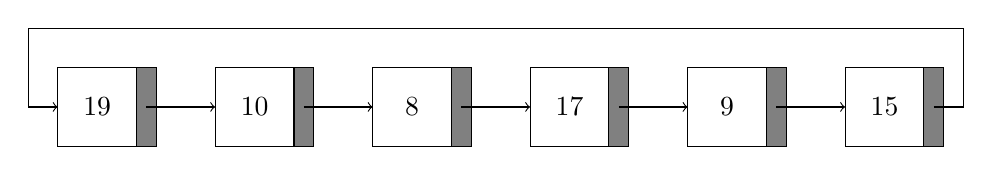
\begin{tikzpicture}[scale=1]
                % Draw the nodes of the circular linked list
                \draw (0, 0) rectangle (1, 1);
                \node at (0.5, 0.5) {19};
                \draw[fill=gray] (1, 1) rectangle (1.25, 0);
        
                \draw (2, 0) rectangle (3, 1);
                \node at (2.5, 0.5) {10};
                \draw[fill=gray] (3, 1) rectangle (3.25, 0);
        
                \draw (4, 0) rectangle (5, 1);
                \node at (4.5, 0.5) {8};
                \draw[fill=gray] (5, 1) rectangle (5.25, 0);
        
                \draw (6, 0) rectangle (7, 1);
                \node at (6.5, 0.5) {17};
                \draw[fill=gray] (7, 1) rectangle (7.25, 0);
        
                \draw (8, 0) rectangle (9, 1);
                \node at (8.5, 0.5) {9};
                \draw[fill=gray] (9, 1) rectangle (9.25, 0);
        
                \draw (10, 0) rectangle (11, 1);
                \node at (10.5, 0.5) {15};
                \draw[fill=gray] (11, 1) rectangle (11.25, 0);
        
                % Draw the arrows between the nodes
                \draw[->] (1.125, 0.5) -- (2, 0.5);
                \draw[->] (3.125, 0.5) -- (4, 0.5);
                \draw[->] (5.125, 0.5) -- (6, 0.5);
                \draw[->] (7.125, 0.5) -- (8, 0.5);
                \draw[->] (9.125, 0.5) -- (10, 0.5);
        
                % Add Curved Arrow from last node to first node
                % \draw[->] (11.125, 0.5) to [out=45, in=135] (0, 0.5);
                \draw[->] (11.125, 0.5)
                    -- (11.5, 0.5)
                    -- (11.5, 1.5)
                    -- (-0.375, 1.5)
                    -- (-0.375, 0.5)
                    -- (0, 0.5);
            \end{tikzpicture}
        \end{center}
        \item Using \textit{cin}, take the input element to search for
        \begin{align*}
            \text{Search Element: 21}
        \end{align*}
        \item Search for the element in the circular linked list
        \begin{align*}
            \text{Output: Element not found.}
        \end{align*}
        \item Determine the \textbf{time complexity} and
        \textbf{space complexity} of the program.
    \end{enumerate}
\end{enumerate}

 %%%%%%%%%%%%%%%%%%%%%%%%%%%%%%%%%%%%
%%%%%~ NEW CHAPTER STARTS HERE %%%%%
%%%%%%%%%%%%%%%%%%%%%%%%%%%%%%%%%%%%
\chapter{Stacks and Queues}

\section{Introduction}

`Stack' and `Queue' are two fundamental data structures in computer
science that are used to store and manage data in a specific order.
They are widely used in various applications, such as operating systems,
compilers, and network protocols, to manage data efficiently.

\section{Stack}

A `Stack' is a linear data structure that follows the Last In First Out
(LIFO) principle, where the last element inserted is the first one to be
removed. The operations on a stack are `Push' (to insert an element),
`Pop' (to remove an element), `Top' (to get the top element), `Size'
(to get the number of elements), and `Empty' (to check if the stack is
empty).

% Draw a stack data structure using TikZ
\begin{figure}[h]
    \centering
    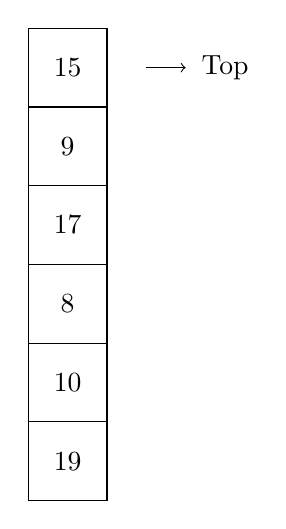
\begin{tikzpicture}
        % Draw the stack data structure
        \draw (0, 0) rectangle (1, 1);
        \node at (0.5, 0.5) {19};
        \draw (0, 1) -- (1, 1);
        \draw (0, 0) -- (0, 1);
        \draw (1, 0) -- (1, 1);

        \draw (0, 1) rectangle (1, 2);
        \node at (0.5, 1.5) {10};
        \draw (0, 2) -- (1, 2);
        \draw (0, 1) -- (0, 2);
        \draw (1, 1) -- (1, 2);

        \draw (0, 2) rectangle (1, 3);
        \node at (0.5, 2.5) {8};
        \draw (0, 3) -- (1, 3);
        \draw (0, 2) -- (0, 3);
        \draw (1, 2) -- (1, 3);

        \draw (0, 3) rectangle (1, 4);
        \node at (0.5, 3.5) {17};
        \draw (0, 4) -- (1, 4);
        \draw (0, 3) -- (0, 4);
        \draw (1, 3) -- (1, 4);

        \draw (0, 4) rectangle (1, 5);
        \node at (0.5, 4.5) {9};
        \draw (0, 5) -- (1, 5);
        \draw (0, 4) -- (0, 5);
        \draw (1, 4) -- (1, 5);

        \draw (0, 5) rectangle (1, 6);
        \node at (0.5, 5.5) {15};
        \draw (0, 6) -- (1, 6);
        \draw (0, 5) -- (0, 6);
        \draw (1, 5) -- (1, 6);
        
        % Add the top pointer
        \draw[->] (1.5, 5.5) -- (2, 5.5);
        \node at (2.5, 5.5) {Top};
    \end{tikzpicture}
    \caption{Stack Data Structure}
    \label{fig:stack-data-structure}
\end{figure}

Figure \ref{fig:stack-data-structure} shows the visual representation of a
stack data structure. The stack contains elements 19, 10, 8, 17, 9, and 15,
where 15 is the top element of the stack.

\subsection{Operations on Stack}

\subsubsection{Push}

The `Push' operation is used to insert an element into the stack. The new
element is added to the top of the stack.

% Draw the Stack for each Push operation for a total of 6 pushes
\begin{figure}[h]
    \centering
    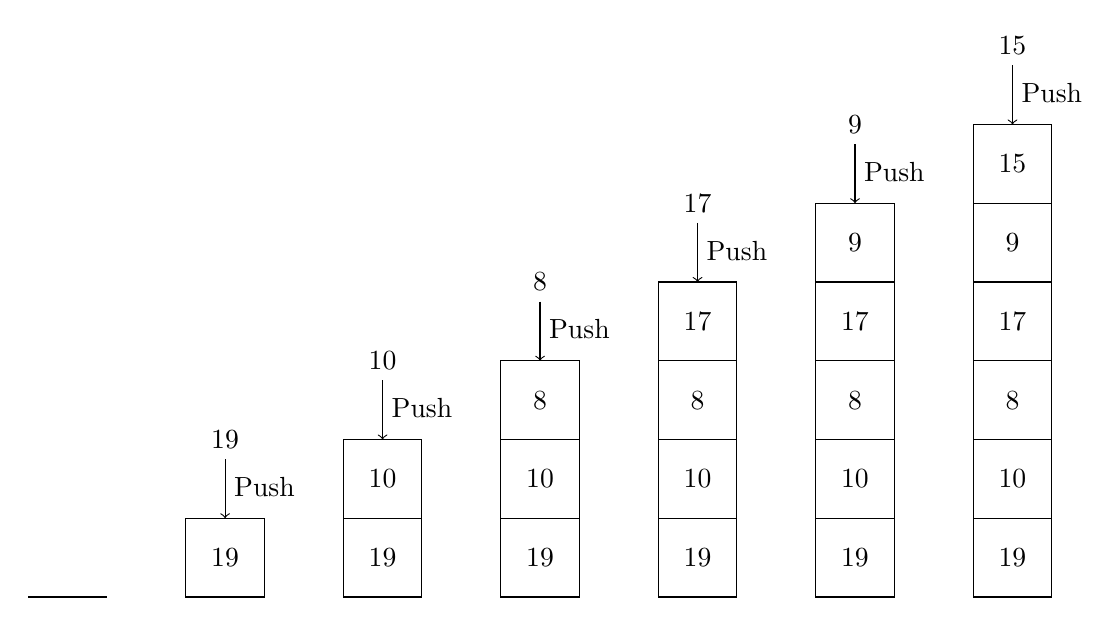
\begin{tikzpicture}
        % Draw a line for initial stack
        \draw (0, 0) -- (1, 0);

        % Draw the stack after first push
        \draw (2, 0) rectangle (3, 1);
        \node at (2.5, 0.5) {19};
        \node at (2.5, 2) {19};
        \draw[->] (2.5, 1.75) -- (2.5, 1);
        \node at (3, 1.4) {Push};

        % Draw the stack after second push
        \draw (4, 0) rectangle (5, 1);
        \node at (4.5, 0.5) {19};

        \draw (4, 1) rectangle (5, 2);
        \node at (4.5, 1.5) {10};
        \node at (4.5, 3) {10};
        \draw[->] (4.5, 2.75) -- (4.5, 2);
        \node at (5, 2.4) {Push};

        % Draw the stack after third push
        \draw (6, 0) rectangle (7, 1);
        \node at (6.5, 0.5) {19};
        \draw (6, 1) rectangle (7, 2);
        \node at (6.5, 1.5) {10};

        \draw (6, 2) rectangle (7, 3);
        \node at (6.5, 2.5) {8};
        \node at (6.5, 4) {8};
        \draw[->] (6.5, 3.75) -- (6.5, 3);
        \node at (7, 3.4) {Push};

        % Draw the stack after fourth push
        \draw (8, 0) rectangle (9, 1);
        \node at (8.5, 0.5) {19};
        \draw (8, 1) rectangle (9, 2);
        \node at (8.5, 1.5) {10};
        \draw (8, 2) rectangle (9, 3);
        \node at (8.5, 2.5) {8};

        \draw (8, 3) rectangle (9, 4);
        \node at (8.5, 3.5) {17};
        \node at (8.5, 5) {17};
        \draw[->] (8.5, 4.75) -- (8.5, 4);
        \node at (9, 4.4) {Push};

        % Draw the stack after fifth push
        \draw (10, 0) rectangle (11, 1);
        \node at (10.5, 0.5) {19};
        \draw (10, 1) rectangle (11, 2);
        \node at (10.5, 1.5) {10};
        \draw (10, 2) rectangle (11, 3);
        \node at (10.5, 2.5) {8};
        \draw (10, 3) rectangle (11, 4);
        \node at (10.5, 3.5) {17};

        \draw (10, 4) rectangle (11, 5);
        \node at (10.5, 4.5) {9};
        \node at (10.5, 6) {9};
        \draw[->] (10.5, 5.75) -- (10.5, 5);
        \node at (11, 5.4) {Push};

        % Draw the stack after sixth push
        \draw (12, 0) rectangle (13, 1);
        \node at (12.5, 0.5) {19};
        \draw (12, 1) rectangle (13, 2);
        \node at (12.5, 1.5) {10};
        \draw (12, 2) rectangle (13, 3);
        \node at (12.5, 2.5) {8};
        \draw (12, 3) rectangle (13, 4);
        \node at (12.5, 3.5) {17};
        \draw (12, 4) rectangle (13, 5);
        \node at (12.5, 4.5) {9};

        \draw (12, 5) rectangle (13, 6);
        \node at (12.5, 5.5) {15};
        \node at (12.5, 7) {15};
        \draw[->] (12.5, 6.75) -- (12.5, 6);
        \node at (13, 6.4) {Push};

        \end{tikzpicture}
    \caption{Stack Push Operation}
    \label{fig:stack-push-operation}
\end{figure}

Figure \ref{fig:stack-push-operation} shows the visual representation of the
`Push' operation on a stack. The stack is initially empty, and elements 19, 10,
8, 17, 9, and 15 are pushed onto the stack one by one.

% Code example for stack push operation
\begin{lstlisting}[language=C++, caption={Stack Push Operation}, label={lst:stack-push-operation}]
#include <iostream>
#include <stack>
using namespace std;

int main() {
    stack<int> s;

    s.push(19);
    s.push(10);
    s.push(8);
    s.push(17);
    s.push(9);
    s.push(15);

    return 0;
}
\end{lstlisting}

Code \ref{lst:stack-push-operation} shows the code for the `Push' operation on
a stack in C++. The code snippet creates a stack using the \texttt{stack} class
from the Standard Template Library (STL) and pushes elements 19, 10, 8, 17, 9,
and 15 onto the stack. To `push' an element onto the stack, the \texttt{push()}
method is called with the element to be inserted as an argument.

\subsubsection{Pop}

The `Pop' operation is used to remove the top element from the stack. The
element is removed from the top of the stack, and the stack is adjusted
accordingly.

% Draw the Stack for each Pop operation for a total of 6 pops
\begin{figure}[h]
    \centering
    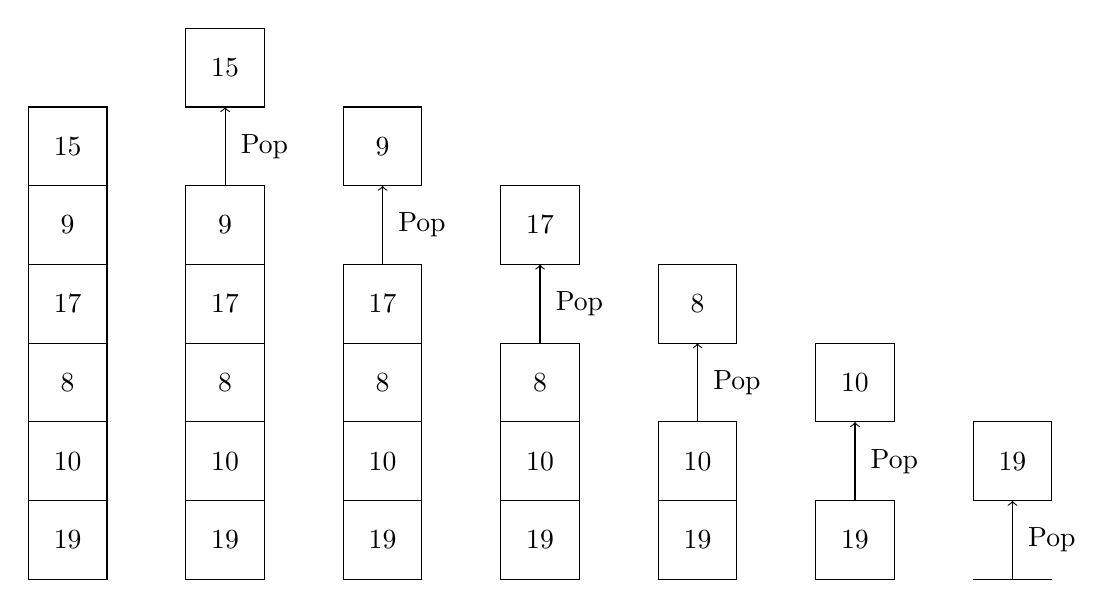
\begin{tikzpicture}
        % Draw the initial stack after all Push operations
        \draw (0, 0) rectangle (1, 1);
        \node at (0.5, 0.5) {19};
        \draw (0, 1) rectangle (1, 2);
        \node at (0.5, 1.5) {10};
        \draw (0, 2) rectangle (1, 3);
        \node at (0.5, 2.5) {8};
        \draw (0, 3) rectangle (1, 4);
        \node at (0.5, 3.5) {17};
        \draw (0, 4) rectangle (1, 5);
        \node at (0.5, 4.5) {9};
        \draw (0, 5) rectangle (1, 6);
        \node at (0.5, 5.5) {15};

        % Draw the stack after first pop
        \draw (2, 0) rectangle (3, 1);
        \node at (2.5, 0.5) {19};
        \draw (2, 1) rectangle (3, 2);
        \node at (2.5, 1.5) {10};
        \draw (2, 2) rectangle (3, 3);
        \node at (2.5, 2.5) {8};
        \draw (2, 3) rectangle (3, 4);
        \node at (2.5, 3.5) {17};
        \draw (2, 4) rectangle (3, 5);
        \node at (2.5, 4.5) {9};

        \draw (2, 6) rectangle (3, 7);
        \node at (2.5, 6.5) {15};
        \draw[->] (2.5, 5) -- (2.5, 6);
        \node at (3, 5.5) {Pop};

        % Draw the stack after second pop
        \draw (4, 0) rectangle (5, 1);
        \node at (4.5, 0.5) {19};
        \draw (4, 1) rectangle (5, 2);
        \node at (4.5, 1.5) {10};
        \draw (4, 2) rectangle (5, 3);
        \node at (4.5, 2.5) {8};
        \draw (4, 3) rectangle (5, 4);
        \node at (4.5, 3.5) {17};
        
        \draw (4, 5) rectangle (5, 6);
        \node at (4.5, 5.5) {9};
        \draw[->] (4.5, 4) -- (4.5, 5);
        \node at (5, 4.5) {Pop};

        % Draw the stack after third pop
        \draw (6, 0) rectangle (7, 1);
        \node at (6.5, 0.5) {19};
        \draw (6, 1) rectangle (7, 2);
        \node at (6.5, 1.5) {10};
        \draw (6, 2) rectangle (7, 3);
        \node at (6.5, 2.5) {8};
        
        \draw (6, 4) rectangle (7, 5);
        \node at (6.5, 4.5) {17};
        \draw[->] (6.5, 3) -- (6.5, 4);
        \node at (7, 3.5) {Pop};

        % Draw the stack after fourth pop
        \draw (8, 0) rectangle (9, 1);
        \node at (8.5, 0.5) {19};
        \draw (8, 1) rectangle (9, 2);
        \node at (8.5, 1.5) {10};

        \draw (8, 3) rectangle (9, 4);
        \node at (8.5, 3.5) {8};
        \draw[->] (8.5, 2) -- (8.5, 3);
        \node at (9, 2.5) {Pop};

        % Draw the stack after fifth pop
        \draw (10, 0) rectangle (11, 1);
        \node at (10.5, 0.5) {19};

        \draw (10, 2) rectangle (11, 3);
        \node at (10.5, 2.5) {10};
        \draw[->] (10.5, 1) -- (10.5, 2);
        \node at (11, 1.5) {Pop};

        % Draw the stack after sixth pop
        \draw (12, 0) -- (13, 0);

        \draw (12, 1) rectangle (13, 2);
        \node at (12.5, 1.5) {19};
        \draw[->] (12.5, 0) -- (12.5, 1);
        \node at (13, 0.5) {Pop};
    \end{tikzpicture}
    \caption{Stack Pop Operation}
    \label{fig:stack-pop-operation}
\end{figure}

Figure \ref{fig:stack-pop-operation} shows the visual representation of the
`Pop' operation on a stack. The stack contains elements 19, 10, 8, 17, 9, and
15, and each element is popped from the stack one by one.

% Code example for stack pop operation
\begin{lstlisting}[language=C++, caption={Stack Pop Operation}, label={lst:stack-pop-operation}]
#include <iostream>
#include <stack>
using namespace std;

int main() {
    stack<int> s = stack<int>({19, 10, 8, 17, 9, 15});

    s.pop(); // Remove 15
    s.pop(); // Remove 9
    s.pop(); // Remove 17
    s.pop(); // Remove 8
    s.pop(); // Remove 10
    s.pop(); // Remove 19

    return 0;
}
\end{lstlisting}

Code \ref{lst:stack-pop-operation} shows the code for the `Pop' operation on
a stack in C++. The code snippet creates a stack using the \texttt{stack} class
from the Standard Template Library (STL) and initializes it with elements 19,
10, 8, 17, 9, and 15. The elements are then popped from the stack one by one
using the \texttt{pop()} method.

\subsubsection{Top}

The `Top' operation is used to get the top element of the stack without
removing it from the stack.

% Draw the Stack for the Top operation
\begin{figure}[h]
    \centering
    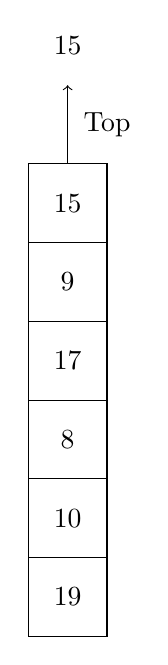
\begin{tikzpicture}
        % Draw the initial stack after all Push operations
        \draw (0, 0) rectangle (1, 1);
        \node at (0.5, 0.5) {19};
        \draw (0, 1) rectangle (1, 2);
        \node at (0.5, 1.5) {10};
        \draw (0, 2) rectangle (1, 3);
        \node at (0.5, 2.5) {8};
        \draw (0, 3) rectangle (1, 4);
        \node at (0.5, 3.5) {17};
        \draw (0, 4) rectangle (1, 5);
        \node at (0.5, 4.5) {9};
        \draw (0, 5) rectangle (1, 6);
        \node at (0.5, 5.5) {15};

        % Draw the stack after Top operation
        \node at (0.5, 7.5) {15};
        \draw[->] (0.5, 6) -- (0.5, 7);
        \node at (1, 6.5) {Top};
    \end{tikzpicture}
    \caption{Stack Top Operation}
    \label{fig:stack-top-operation}
\end{figure}

Figure \ref{fig:stack-top-operation} shows the visual representation of the
`Top' operation on a stack. The stack contains elements 19, 10, 8, 17, 9, and
15, and the top element of the stack is 15.

% Code example for stack top operation
\begin{lstlisting}[language=C++, caption={Stack Top Operation}, label={lst:stack-top-operation}]
#include <iostream>
#include <stack>
using namespace std;

int main() {
    stack<int> s = stack<int>({19, 10, 8, 17, 9, 15});

    cout << "Top Element: " << s.top() << endl;

    return 0;
}
\end{lstlisting}

Code \ref{lst:stack-top-operation} shows the code for the `Top' operation on
a stack in C++. The code snippet creates a stack using the \texttt{stack} class
from the Standard Template Library (STL) and initializes it with elements 19,
10, 8, 17, 9, and 15. To get the top element of the stack, the \texttt{top()}
method is called.

\subsubsection{Size}

The `Size' operation is used to get the number of elements in the stack.

% Draw the Stack for the Size operation
\begin{figure}[h]
    \centering
    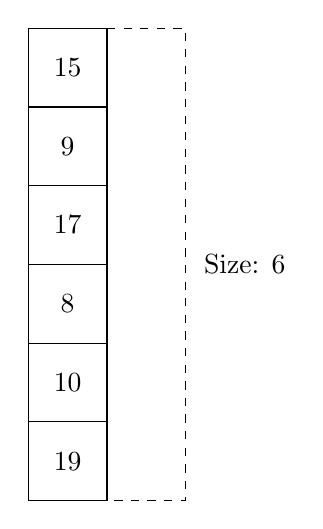
\begin{tikzpicture}
        % Draw the initial stack after all Push operations
        \draw (0, 0) rectangle (1, 1);
        \node at (0.5, 0.5) {19};
        \draw (0, 1) rectangle (1, 2);
        \node at (0.5, 1.5) {10};
        \draw (0, 2) rectangle (1, 3);
        \node at (0.5, 2.5) {8};
        \draw (0, 3) rectangle (1, 4);
        \node at (0.5, 3.5) {17};
        \draw (0, 4) rectangle (1, 5);
        \node at (0.5, 4.5) {9};
        \draw (0, 5) rectangle (1, 6);
        \node at (0.5, 5.5) {15};

        % Draw the stack after Size operation
        \draw[dashed] (1, 6) -- (2, 6) -- (2, 0) -- (1, 0);
        \node at (2.75, 3) {Size: 6};
    \end{tikzpicture}
    \caption{Stack Size Operation}
    \label{fig:stack-size-operation}
\end{figure}

Figure \ref{fig:stack-size-operation} shows the visual representation of the
`Size' operation on a stack. The stack contains elements 19, 10, 8, 17, 9, and
15, and the size of the stack is 6.

% Code example for stack size operation
\begin{lstlisting}[language=C++, caption={Stack Size Operation}, label={lst:stack-size-operation}]
#include <iostream>
#include <stack>
using namespace std;

int main() {
    stack<int> s = stack<int>({19, 10, 8, 17, 9, 15});

    cout << "Size of Stack: " << s.size() << endl;

    return 0;
}
\end{lstlisting}

Code \ref{lst:stack-size-operation} shows the code for the `Size' operation on
a stack in C++. The code snippet creates a stack using the \texttt{stack} class
from the Standard Template Library (STL) and initializes it with elements 19,
10, 8, 17, 9, and 15. To get the size of the stack, the \texttt{size()} method
is called.

\subsubsection{Empty}

The `Empty' operation is used to check if the stack is empty or not. It returns
\texttt{true} if the stack is empty and \texttt{false} otherwise.

% Draw the Stack for the Empty operation
\begin{figure}[h]
    \centering
    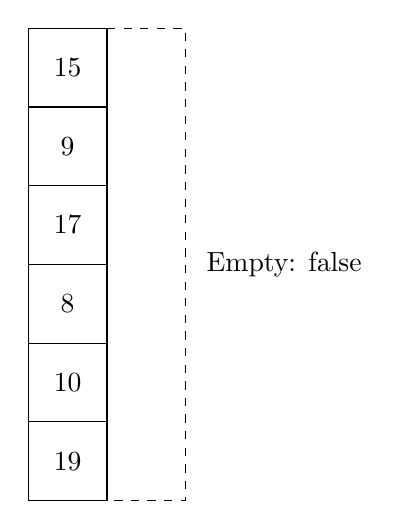
\begin{tikzpicture}
        % Draw the initial stack after all Push operations
        \draw (0, 0) rectangle (1, 1);
        \node at (0.5, 0.5) {19};
        \draw (0, 1) rectangle (1, 2);
        \node at (0.5, 1.5) {10};
        \draw (0, 2) rectangle (1, 3);
        \node at (0.5, 2.5) {8};
        \draw (0, 3) rectangle (1, 4);
        \node at (0.5, 3.5) {17};
        \draw (0, 4) rectangle (1, 5);
        \node at (0.5, 4.5) {9};
        \draw (0, 5) rectangle (1, 6);
        \node at (0.5, 5.5) {15};

        % Draw the stack after Empty operation
        \draw[dashed] (1, 6) -- (2, 6) -- (2, 0) -- (1, 0);
        \node at (3.25, 3) {Empty: false};
    \end{tikzpicture}
    \caption{Stack Empty Operation}
    \label{fig:stack-empty-operation}
\end{figure}

Figure \ref{fig:stack-empty-operation} shows the visual representation of the
`Empty' operation on a stack. The stack contains elements 19, 10, 8, 17, 9, and
15, and the stack is not empty.

% Code example for stack empty operation
\begin{lstlisting}[language=C++, caption={Stack Empty Operation}, label={lst:stack-empty-operation}]
#include <iostream>
#include <stack>
using namespace std;

int main() {
    stack<int> s = stack<int>({19, 10, 8, 17, 9, 15});

    cout << "Is Stack Empty: " << (s.empty() ? "true" : "false") << endl;

    return 0;
}
\end{lstlisting}

Code \ref{lst:stack-empty-operation} shows the code for the `Empty' operation on
a stack in C++. The code snippet creates a stack using the \texttt{stack} class
from the Standard Template Library (STL) and initializes it with elements 19,
10, 8, 17, 9, and 15. To check if the stack is empty, the \texttt{empty()}
method is called.

% \subsection{Complexity Analysis of Stack}

% The time complexity of the `Push', `Pop', `Top', `Size', and `Empty' operations
% on a stack is $O(1)$, as they involve only a single operation to insert, remove,
% get the top element, get the size, and check if the stack is empty, respectively.
% The space complexity of a stack is $O(n)$, where $n$ is the number of elements in
% the stack, as it requires memory to store the elements.

% % \subsection{Implementation of Stack Using Arrays}

% % \subsection{Implementation of Stack Using Linked Lists}

\section{Queue}

A `Queue' is a linear data structure that follows the First In First Out
(FIFO) principle, where the first element inserted is the first one to be
removed. The operations on a queue are `Push' (to insert an element),
`Pop' (to remove an element), `Front' (to get the front element),
`Back' (to get the back element), `Size' (to get the number of elements),
and `Empty' (to check if the queue is empty).

% One particular application of a queue is in the scheduling of processes in
% an operating system. The processes are added to the queue in the order they
% arrive and are executed in the same order.

% Draw a queue data structure using TikZ
\begin{figure}[h]
    \centering
    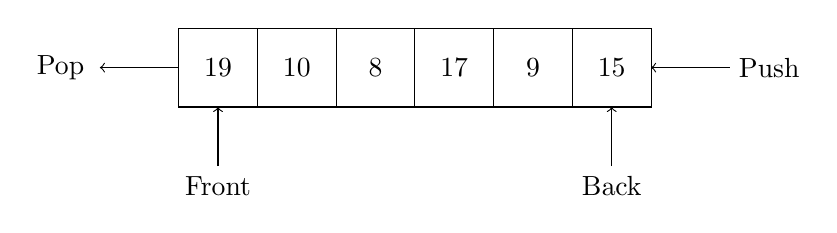
\begin{tikzpicture}
        % Draw the queue data structure
        \draw (0, 0) rectangle (1, 1);
        \node at (0.5, 0.5) {19};
        \draw (1, 0) rectangle (2, 1);
        \node at (1.5, 0.5) {10};
        \draw (2, 0) rectangle (3, 1);
        \node at (2.5, 0.5) {8};
        \draw (3, 0) rectangle (4, 1);
        \node at (3.5, 0.5) {17};
        \draw (4, 0) rectangle (5, 1);
        \node at (4.5, 0.5) {9};
        \draw (5, 0) rectangle (6, 1);
        \node at (5.5, 0.5) {15};

        % Add the front and back pointers
        \draw[->] (0.5, -0.75) -- (0.5, 0);
        \node at (0.5, -1) {Front};
        \draw[->] (5.5, -0.75) -- (5.5, 0);
        \node at (5.5, -1) {Back};

        % Add the Push and Pop pointers
        \draw[->] (0, 0.5) -- (-1, 0.5);
        \node at (-1.5, 0.5) {Pop};
        \draw[->] (7, 0.5) -- (6, 0.5);
        \node at (7.5, 0.5) {Push};
    \end{tikzpicture}
    \caption{Queue Data Structure}
    \label{fig:queue-data-structure}
\end{figure}

Figure \ref{fig:queue-data-structure} shows the visual representation of a
queue data structure. The queue contains elements 19, 10, 8, 17, 9, and 15,
where 19 is the front element and 15 is the back element of the queue.

\subsection{Operations on Queue}

\subsubsection{Push}

The `Push' operation is used to insert an element into the queue. The new
element is added to the back of the queue.

% Draw the Queue for each Push operation for a total of 6 pushes
\begin{figure}[h]
    \centering
    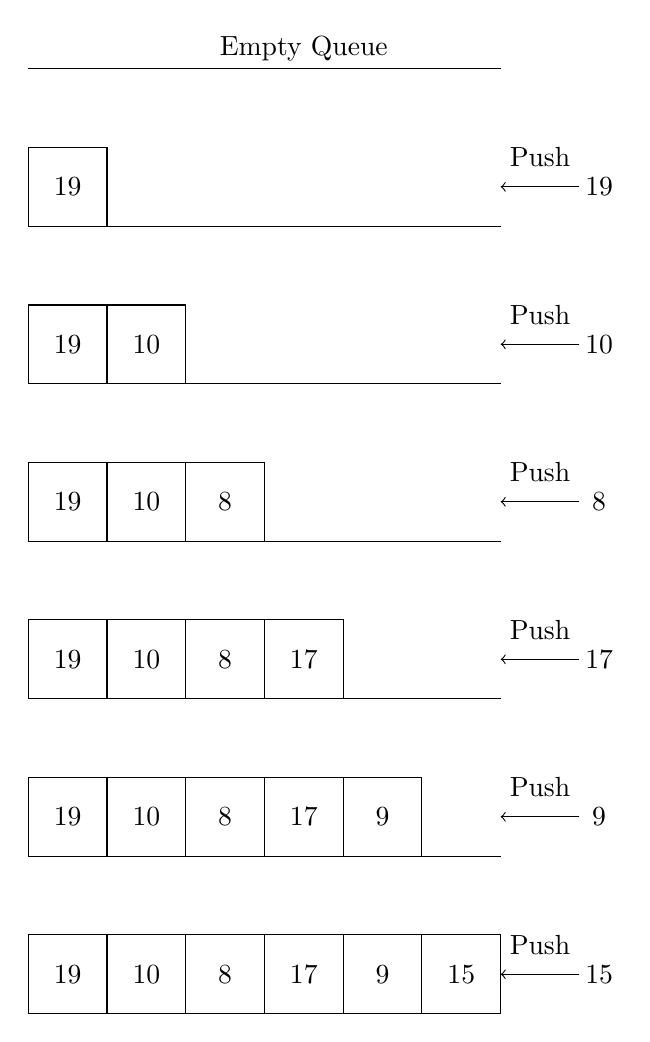
\begin{tikzpicture}
        % Draw a line for initial queue
        \draw (0, 0) -- (6, 0);
        \node at (3.5, 0.25) {Empty Queue};

        % Draw the queue after first push
        \draw (0, -2) -- (6, -2);
        \draw (0, -2) rectangle (1, -1);
        \node at (0.5, -1.5) {19};

        \draw[->] (7, -1.5) -- (6, -1.5);
        \node at (7.25, -1.5) {19};
        \node at (6.5, -1.125) {Push};

        % Draw the queue after second push
        \draw (0, -4) -- (6, -4);
        \draw (0, -4) rectangle (1, -3);
        \node at (0.5, -3.5) {19};
        \draw (1, -4) rectangle (2, -3);
        \node at (1.5, -3.5) {10};

        \draw[->] (7, -3.5) -- (6, -3.5);
        \node at (7.25, -3.5) {10};
        \node at (6.5, -3.125) {Push};

        % Draw the queue after third push
        \draw (0, -6) -- (6, -6);
        \draw (0, -6) rectangle (1, -5);
        \node at (0.5, -5.5) {19};
        \draw (1, -6) rectangle (2, -5);
        \node at (1.5, -5.5) {10};
        \draw (2, -6) rectangle (3, -5);
        \node at (2.5, -5.5) {8};

        \draw[->] (7, -5.5) -- (6, -5.5);
        \node at (7.25, -5.5) {8};
        \node at (6.5, -5.125) {Push};

        % Draw the queue after fourth push
        \draw (0, -8) -- (6, -8);
        \draw (0, -8) rectangle (1, -7);
        \node at (0.5, -7.5) {19};
        \draw (1, -8) rectangle (2, -7);
        \node at (1.5, -7.5) {10};
        \draw (2, -8) rectangle (3, -7);
        \node at (2.5, -7.5) {8};
        \draw (3, -8) rectangle (4, -7);
        \node at (3.5, -7.5) {17};

        \draw[->] (7, -7.5) -- (6, -7.5);
        \node at (7.25, -7.5) {17};
        \node at (6.5, -7.125) {Push};

        % Draw the queue after fifth push
        \draw (0, -10) -- (6, -10);
        \draw (0, -10) rectangle (1, -9);
        \node at (0.5, -9.5) {19};
        \draw (1, -10) rectangle (2, -9);
        \node at (1.5, -9.5) {10};
        \draw (2, -10) rectangle (3, -9);
        \node at (2.5, -9.5) {8};
        \draw (3, -10) rectangle (4, -9);
        \node at (3.5, -9.5) {17};
        \draw (4, -10) rectangle (5, -9);
        \node at (4.5, -9.5) {9};

        \draw[->] (7, -9.5) -- (6, -9.5);
        \node at (7.25, -9.5) {9};
        \node at (6.5, -9.125) {Push};

        % Draw the queue after sixth push
        \draw (0, -12) -- (6, -12);
        \draw (0, -12) rectangle (1, -11);
        \node at (0.5, -11.5) {19};
        \draw (1, -12) rectangle (2, -11);
        \node at (1.5, -11.5) {10};
        \draw (2, -12) rectangle (3, -11);
        \node at (2.5, -11.5) {8};
        \draw (3, -12) rectangle (4, -11);
        \node at (3.5, -11.5) {17};
        \draw (4, -12) rectangle (5, -11);
        \node at (4.5, -11.5) {9};
        \draw (5, -12) rectangle (6, -11);
        \node at (5.5, -11.5) {15};

        \draw[->] (7, -11.5) -- (6, -11.5);
        \node at (7.25, -11.5) {15};
        \node at (6.5, -11.125) {Push};
    \end{tikzpicture}
    \caption{Queue Push Operation}
    \label{fig:queue-push-operation}
\end{figure}

Figure \ref{fig:queue-push-operation} shows the visual representation of the
`Push' operation on a queue. The queue is initially empty, and elements 19, 10,
8, 17, 9, and 15 are pushed into the queue one by one.

% Code example for queue push operation
\begin{lstlisting}[language=C++, caption={Queue Push Operation}, label={lst:queue-push-operation}]
#include <iostream>
#include <queue>
using namespace std;

int main() {
    queue<int> q;

    q.push(19);
    q.push(10);
    q.push(8);
    q.push(17);
    q.push(9);
    q.push(15);

    return 0;
}
\end{lstlisting}

Code \ref{lst:queue-push-operation} shows the code for the `Push' operation on
a queue in C++. The code snippet creates a queue using the \texttt{queue} class
from the Standard Template Library (STL) and pushes elements 19, 10, 8, 17, 9,
and 15 into the queue. To `push' an element into the queue, the \texttt{push()}
method is called with the element to be inserted as an argument.

\subsubsection{Pop}

The `Pop' operation is used to remove the front element from the queue. The
element is removed from the front of the queue, and the queue is adjusted
accordingly.

% Draw the Queue for each Pop operation for a total of 6 pops
\begin{figure}[h]
    \centering
    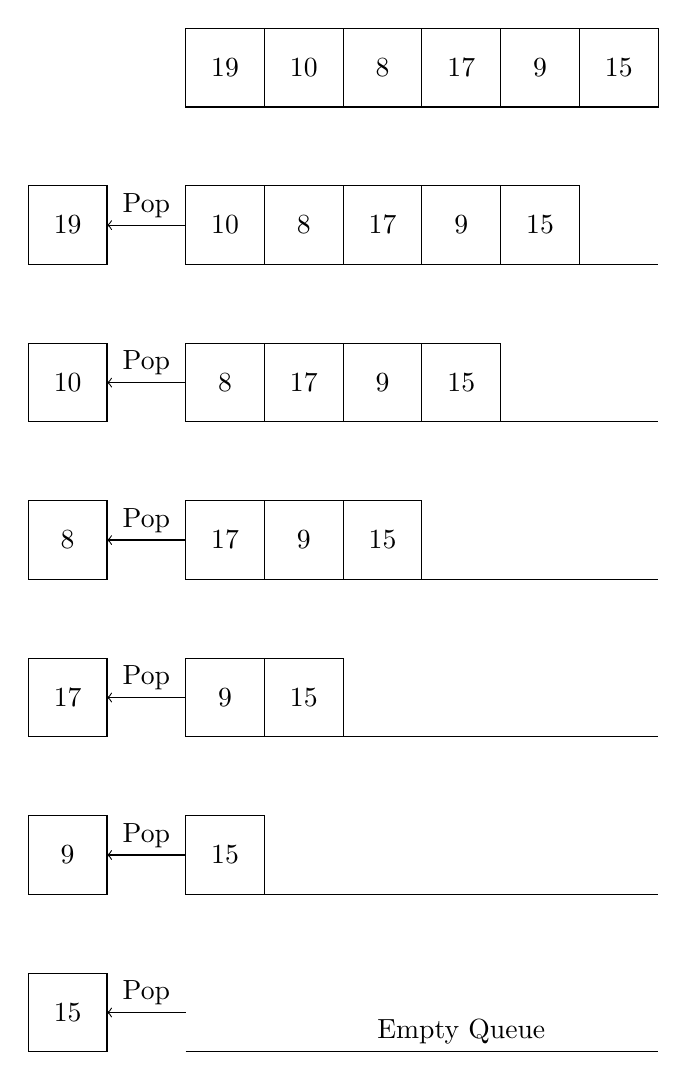
\begin{tikzpicture}
        % Draw the initial queue after all Push operations
        \draw (0, 0) -- (6, 0);
        \draw (0, 0) rectangle (1, 1);
        \node at (0.5, 0.5) {19};
        \draw (1, 0) rectangle (2, 1);
        \node at (1.5, 0.5) {10};
        \draw (2, 0) rectangle (3, 1);
        \node at (2.5, 0.5) {8};
        \draw (3, 0) rectangle (4, 1);
        \node at (3.5, 0.5) {17};
        \draw (4, 0) rectangle (5, 1);
        \node at (4.5, 0.5) {9};
        \draw (5, 0) rectangle (6, 1);
        \node at (5.5, 0.5) {15};
        
        % Draw the queue after first pop
        \draw (0, -2) -- (6, -2);
        \draw (0, -2) rectangle (1, -1);
        \node at (0.5, -1.5) {10};
        \draw (1, -2) rectangle (2, -1);
        \node at (1.5, -1.5) {8};
        \draw (2, -2) rectangle (3, -1);
        \node at (2.5, -1.5) {17};
        \draw (3, -2) rectangle (4, -1);
        \node at (3.5, -1.5) {9};
        \draw (4, -2) rectangle (5, -1);
        \node at (4.5, -1.5) {15};
        
        \draw[->] (0, -1.5) -- (-1, -1.5);
        \node at (-0.5, -1.25) {Pop};
        \draw (-1, -2) rectangle (-2, -1);
        \node at (-1.5, -1.5) {19};

        % Draw the queue after second pop
        \draw (0, -4) -- (6, -4);
        \draw (0, -4) rectangle (1, -3);
        \node at (0.5, -3.5) {8};
        \draw (1, -4) rectangle (2, -3);
        \node at (1.5, -3.5) {17};
        \draw (2, -4) rectangle (3, -3);
        \node at (2.5, -3.5) {9};
        \draw (3, -4) rectangle (4, -3);
        \node at (3.5, -3.5) {15};

        \draw[->] (0, -3.5) -- (-1, -3.5);
        \node at (-0.5, -3.25) {Pop};
        \draw (-1, -4) rectangle (-2, -3);
        \node at (-1.5, -3.5) {10};

        % Draw the queue after third pop
        \draw (0, -6) -- (6, -6);
        \draw (0, -6) rectangle (1, -5);
        \node at (0.5, -5.5) {17};
        \draw (1, -6) rectangle (2, -5);
        \node at (1.5, -5.5) {9};
        \draw (2, -6) rectangle (3, -5);
        \node at (2.5, -5.5) {15};

        \draw[->] (0, -5.5) -- (-1, -5.5);
        \node at (-0.5, -5.25) {Pop};
        \draw (-1, -6) rectangle (-2, -5);
        \node at (-1.5, -5.5) {8};

        % Draw the queue after fourth pop
        \draw (0, -8) -- (6, -8);
        \draw (0, -8) rectangle (1, -7);
        \node at (0.5, -7.5) {9};
        \draw (1, -8) rectangle (2, -7);
        \node at (1.5, -7.5) {15};

        \draw[->] (0, -7.5) -- (-1, -7.5);
        \node at (-0.5, -7.25) {Pop};
        \draw (-1, -8) rectangle (-2, -7);
        \node at (-1.5, -7.5) {17};

        % Draw the queue after fifth pop
        \draw (0, -10) -- (6, -10);
        \draw (0, -10) rectangle (1, -9);
        \node at (0.5, -9.5) {15};

        \draw[->] (0, -9.5) -- (-1, -9.5);
        \node at (-0.5, -9.25) {Pop};
        \draw (-1, -10) rectangle (-2, -9);
        \node at (-1.5, -9.5) {9};

        % Draw the queue after sixth pop
        \draw (0, -12) -- (6, -12);
        \node at (3.5, -11.75) {Empty Queue};

        \draw[->] (0, -11.5) -- (-1, -11.5);
        \node at (-0.5, -11.25) {Pop};
        \draw (-1, -12) rectangle (-2, -11);
        \node at (-1.5, -11.5) {15};
    \end{tikzpicture}
    \caption{Queue Pop Operation}
    \label{fig:queue-pop-operation}
\end{figure}

Figure \ref{fig:queue-pop-operation} shows the visual representation of the
`Pop' operation on a queue. The queue contains elements 19, 10, 8, 17, 9, and
15, and each element is popped from the queue one by one.

% Code example for queue pop operation
\begin{lstlisting}[language=C++, caption={Queue Pop Operation}, label={lst:queue-pop-operation}]
#include <iostream>
#include <queue>
using namespace std;

int main() {
    queue<int> q = queue<int>({19, 10, 8, 17, 9, 15});

    q.pop(); // Remove 19
    q.pop(); // Remove 10
    q.pop(); // Remove 8
    q.pop(); // Remove 17
    q.pop(); // Remove 9
    q.pop(); // Remove 15

    return 0;
}
\end{lstlisting}

Code \ref{lst:queue-pop-operation} shows the code for the `Pop' operation on
a queue in C++. The code snippet creates a queue using the \texttt{queue} class
from the Standard Template Library (STL) and initializes it with elements 19,
10, 8, 17, 9, and 15. The elements are then popped from the queue one by one
using the \texttt{pop()} method.

\subsubsection{Front}

The `Front' operation is used to get the front element of the queue without
removing it from the queue.

% Draw the Queue for the Front operation
\begin{figure}[h]
    \centering
    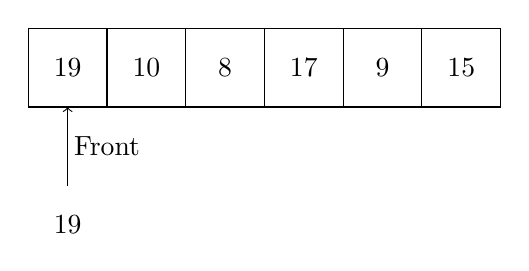
\begin{tikzpicture}
        % Draw the initial queue after all Push operations
        \draw (0, 0) rectangle (1, 1);
        \node at (0.5, 0.5) {19};
        \draw (1, 0) rectangle (2, 1);
        \node at (1.5, 0.5) {10};
        \draw (2, 0) rectangle (3, 1);
        \node at (2.5, 0.5) {8};
        \draw (3, 0) rectangle (4, 1);
        \node at (3.5, 0.5) {17};
        \draw (4, 0) rectangle (5, 1);
        \node at (4.5, 0.5) {9};
        \draw (5, 0) rectangle (6, 1);
        \node at (5.5, 0.5) {15};

        % Draw the queue after Front operation
        \node at (0.5, -1.5) {19};
        \draw[->] (0.5, -1) -- (0.5, 0);
        \node at (1, -0.5) {Front};
    \end{tikzpicture}
    \caption{Queue Front Operation}
    \label{fig:queue-front-operation}
\end{figure}

Figure \ref{fig:queue-front-operation} shows the visual representation of the
`Front' operation on a queue. The queue contains elements 19, 10, 8, 17, 9, and
15, and the front element of the queue is 19.

% Code example for queue front operation
\begin{lstlisting}[language=C++, caption={Queue Front Operation}, label={lst:queue-front-operation}]
#include <iostream>
#include <queue>
using namespace std;

int main() {
    queue<int> q = queue<int>({19, 10, 8, 17, 9, 15});

    cout << "Front Element: " << q.front() << endl;

    return 0;
}
\end{lstlisting}

Code \ref{lst:queue-front-operation} shows the code for the `Front' operation on
a queue in C++. The code snippet creates a queue using the \texttt{queue} class
from the Standard Template Library (STL) and initializes it with elements 19,
10, 8, 17, 9, and 15. To get the front element of the queue, the \texttt{front()}
method is called.

\subsubsection{Back}

The `Back' operation is used to get the back element of the queue without
removing it from the queue.

% Draw the Queue for the Back operation
\begin{figure}[h]
    \centering
    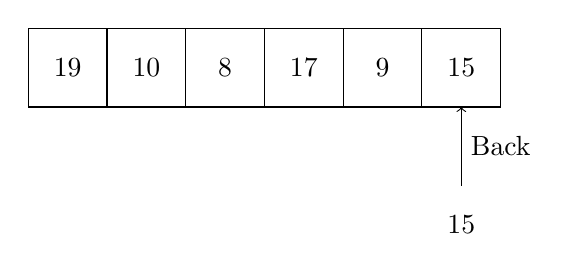
\begin{tikzpicture}
        % Draw the initial queue after all Push operations
        \draw (0, 0) rectangle (1, 1);
        \node at (0.5, 0.5) {19};
        \draw (1, 0) rectangle (2, 1);
        \node at (1.5, 0.5) {10};
        \draw (2, 0) rectangle (3, 1);
        \node at (2.5, 0.5) {8};
        \draw (3, 0) rectangle (4, 1);
        \node at (3.5, 0.5) {17};
        \draw (4, 0) rectangle (5, 1);
        \node at (4.5, 0.5) {9};
        \draw (5, 0) rectangle (6, 1);
        \node at (5.5, 0.5) {15};

        % Draw the queue after Back operation
        \node at (5.5, -1.5) {15};
        \draw[->] (5.5, -1) -- (5.5, 0);
        \node at (6, -0.5) {Back};
    \end{tikzpicture}
    \caption{Queue Back Operation}
    \label{fig:queue-back-operation}
\end{figure}

Figure \ref{fig:queue-back-operation} shows the visual representation of the
`Back' operation on a queue. The queue contains elements 19, 10, 8, 17, 9, and
15, and the back element of the queue is 15.

% Code example for queue back operation
\begin{lstlisting}[language=C++, caption={Queue Back Operation}, label={lst:queue-back-operation}]
#include <iostream>
#include <queue>
using namespace std;

int main() {
    queue<int> q = queue<int>({19, 10, 8, 17, 9, 15});

    cout << "Back Element: " << q.back() << endl;

    return 0;
}
\end{lstlisting}

Code \ref{lst:queue-back-operation} shows the code for the `Back' operation on
a queue in C++. The code snippet creates a queue using the \texttt{queue} class
from the Standard Template Library (STL) and initializes it with elements 19,
10, 8, 17, 9, and 15. To get the back element of the queue, the \texttt{back()}
method is called.

\subsubsection{Size}

The `Size' operation is used to get the number of elements in the queue.

% Draw the Queue for the Size operation
\begin{figure}[h]
    \centering
    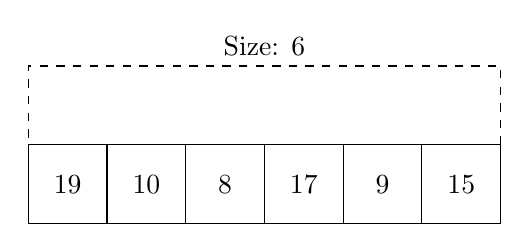
\begin{tikzpicture}
        % Draw the initial queue after all Push operations
        \draw (0, 0) rectangle (1, 1);
        \node at (0.5, 0.5) {19};
        \draw (1, 0) rectangle (2, 1);
        \node at (1.5, 0.5) {10};
        \draw (2, 0) rectangle (3, 1);
        \node at (2.5, 0.5) {8};
        \draw (3, 0) rectangle (4, 1);
        \node at (3.5, 0.5) {17};
        \draw (4, 0) rectangle (5, 1);
        \node at (4.5, 0.5) {9};
        \draw (5, 0) rectangle (6, 1);
        \node at (5.5, 0.5) {15};

        % Draw the queue after Size operation
        \draw[dashed] (6, 1) -- (6, 2) -- (0, 2) -- (0, 1);
        \node at (3, 2.25) {Size: 6};
    \end{tikzpicture}
    \caption{Queue Size Operation}
    \label{fig:queue-size-operation}
\end{figure}

Figure \ref{fig:queue-size-operation} shows the visual representation of the
`Size' operation on a queue. The queue contains elements 19, 10, 8, 17, 9, and
15, and the size of the queue is 6.

% Code example for queue size operation
\begin{lstlisting}[language=C++, caption={Queue Size Operation}, label={lst:queue-size-operation}]
#include <iostream>
#include <queue>
using namespace std;

int main() {
    queue<int> q = queue<int>({19, 10, 8, 17, 9, 15});

    cout << "Size of Queue: " << q.size() << endl;

    return 0;
}
\end{lstlisting}

Code \ref{lst:queue-size-operation} shows the code for the `Size' operation on
a queue in C++. The code snippet creates a queue using the \texttt{queue} class
from the Standard Template Library (STL) and initializes it with elements 19,
10, 8, 17, 9, and 15. To get the size of the queue, the \texttt{size()} method
is called.

\subsubsection{Empty}

The `Empty' operation is used to check if the queue is empty or not. It returns
\texttt{true} if the queue is empty and \texttt{false} otherwise.

% Draw the Queue for the Empty operation
\begin{figure}[h]
    \centering
    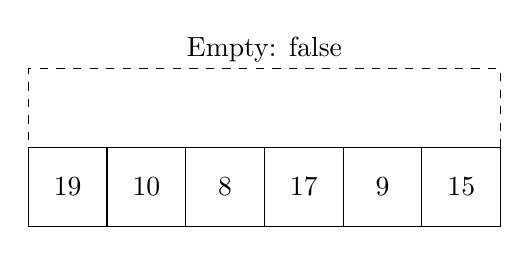
\begin{tikzpicture}
        % Draw the initial queue after all Push operations
        \draw (0, 0) rectangle (1, 1);
        \node at (0.5, 0.5) {19};
        \draw (1, 0) rectangle (2, 1);
        \node at (1.5, 0.5) {10};
        \draw (2, 0) rectangle (3, 1);
        \node at (2.5, 0.5) {8};
        \draw (3, 0) rectangle (4, 1);
        \node at (3.5, 0.5) {17};
        \draw (4, 0) rectangle (5, 1);
        \node at (4.5, 0.5) {9};
        \draw (5, 0) rectangle (6, 1);
        \node at (5.5, 0.5) {15};

        % Draw the queue after Empty operation
        \draw[dashed] (6, 1) -- (6, 2) -- (0, 2) -- (0, 1);
        \node at (3, 2.25) {Empty: false};
    \end{tikzpicture}
    \caption{Queue Empty Operation}
    \label{fig:queue-empty-operation}
\end{figure}

Figure \ref{fig:queue-empty-operation} shows the visual representation of the
`Empty' operation on a queue. The queue contains elements 19, 10, 8, 17, 9, and
15, and the queue is not empty.

% Code example for queue empty operation
\begin{lstlisting}[language=C++, caption={Queue Empty Operation}, label={lst:queue-empty-operation}]
#include <iostream>
#include <queue>
using namespace std;

int main() {
    queue<int> q = queue<int>({19, 10, 8, 17, 9, 15});

    cout << "Is Queue Empty: " << (q.empty() ? "true" : "false") << endl;

    return 0;
}
\end{lstlisting}

Code \ref{lst:queue-empty-operation} shows the code for the `Empty' operation on
a queue in C++. The code snippet creates a queue using the \texttt{queue} class
from the Standard Template Library (STL) and initializes it with elements 19,
10, 8, 17, 9, and 15. To check if the queue is empty, the \texttt{empty()}
method is called.

% \subsection{Complexity Analysis of Queue}

% The time complexity of the `Push', `Pop', `Front', `Back', `Size', and `Empty'
% operations on a queue is $O(1)$. The space complexity of a queue is $O(n)$, where
% $n$ is the number of elements in the queue.

% \subsection{Implementation of Queue Using Arrays}

% \subsection{Implementation of Queue Using Linked Lists}

\section{Comparison of Stack and Queue}

The key differences between a `Stack' and a `Queue' is that a stack follows the
Last In First Out (LIFO) principle, while a queue follows the First In First Out
(FIFO) principle. You can visualize a stack as a stack of plates, where the last
plate added is the first one to be removed. On the other hand, you can visualize
a queue as a line of people waiting for a bus, where the first person in line is
the first one to board the bus.

In `stack' you can only access the top element, while in `queue' you can access
both the front and back elements. In `stack' you can only push and pop elements
at the top, while in `queue' you can push elements at the back and pop elements
from the front. The time complexity of the `push', `pop', `front', `back', `size',
and `empty' operations is the same for both stack and queue. Both also have the
same space complexity. In `stack' you can only access the top element while in
`queue' you can access both the front and back elements.

\section{Summary}

In this chapter, we discussed the `Queue' data structure. A queue is a linear
data structure that follows the First In First Out (FIFO) principle. We learned
about the basic operations on a queue, such as `Push', `Pop', `Front', `Back',
`Size', and `Empty'. We also compared the `Stack' and `Queue' data structures.

%%%%%%%%%%%%%%%%%%%%%%%%%%%%%%%%%%%%
%%%%%~ NEW CHAPTER STARTS HERE %%%%%
%%%%%%%%%%%%%%%%%%%%%%%%%%%%%%%%%%%%
% \chapter{Trees}

% \section{Introduction}

% \section{Properties of Trees}

% \subsection{Root Node}

% \subsection{Parent Node}

% \subsection{Child Node}

% \subsection{Leaf Node}

% \subsection{Ancestors}

% \subsection{Siblings}

% \subsection{Descendants}

% \subsection{Height of a Tree}

% \subsection{Depth of a Node}

% \subsection{Degree of a Node}

% \subsection{Level of a Node}

% \subsection{Subtree}

% \section{Types of Trees}

% \subsection{Binary Tree}

% \subsubsection{Types of Binary Trees}

% \paragraph{Left-skewed Binary Tree}

% \paragraph{Right-skewed Binary Tree}

% \paragraph{Complete Binary Tree}

% \subsection{Ternary Tree}

% \subsection{N-ary Tree}

% \subsection{Binary Search Tree}

% \subsection{AVL Tree}

% \subsection{Red-Black Tree}

% \section{Basic Operations on Trees}

% \subsection{Creation of a Tree}

% \subsection{Insertion}

% \subsection{Deletion}

% \subsection{Searching}

% \subsection{Traversal}

% \subsubsection{Preorder Traversal}

% \subsubsection{Inorder Traversal}

% \subsubsection{Postorder Traversal}

% \subsubsection{Level-order Traversal}

% \section{Complexity Analysis of Trees}

% \section{Summary}

%%%%%%%%%%%%%%%%%%%%%%%%%%%%%%%%%%%%
%%%%%~ NEW CHAPTER STARTS HERE %%%%%
%%%%%%%%%%%%%%%%%%%%%%%%%%%%%%%%%%%%
% \chapter{Graphs}

% \section{Introduction}

% \section{Properties of Graphs}

% \subsection{Vertex}

% \subsection{Edge}

% \subsection{Degree of a Vertex}

% \subsection{Path}

% \section{Types of Graphs}

% \subsection{Finite Graph}

% \subsection{Infinite Graph}

% \subsection{Trivial Graph}

% \subsection{Simple Graph}

% \subsection{Multi Graph}

% \subsection{Null Graph}

% \subsection{Complete Graph}

% \subsection{Pseudo Graph}

% \subsection{Regular Graph}

% \subsection{Bipartite Graph}

% \subsection{Labelled Graph}

% \subsection{Weighted Graph}

% \subsection{Directed Graph}

% \subsection{Undirected Graph}

% \subsection{Connected Graph}

% \subsection{Disconnected Graph}

% \subsection{Cyclic Graph}

% \subsection{Acyclic Graph}

% \subsection{Directed Acyclic Graph (DAG)}

% \subsection{Digraph}

% \subsection{Subgraph}

% \section{Operations on Graphs}

% \subsection{Creation of a Graph}

% \subsection{Insertion}

% \subsubsection{Insertion of a Vertex}

% \subsubsection{Insertion of an Edge}

% \subsection{Deletion}

% \subsubsection{Deletion of a Vertex}

% \subsubsection{Deletion of an Edge}

% \subsection{Traversal}

% \subsubsection{Depth First Search (DFS)}

% \subsubsection{Breadth First Search (BFS)}

% \subsection{Shortest Path}

% \subsection{Minimum Spanning Tree}

% \section{Complexity Analysis of Graphs}

% \section{Summary}

%%%%%%%%%%%%%%%%%%%%%%%%%%%%%%%%%%%%
%%%%%~ NEW CHAPTER STARTS HERE %%%%%
%%%%%%%%%%%%%%%%%%%%%%%%%%%%%%%%%%%%

\chapter{Introduction to Algorithms}

\section{Introduction}

Algorithms are a fundamental concept in computer science and play a crucial role
in solving computational problems efficiently. An algorithm is a step-by-step
procedure or a set of rules to solve a specific problem. It is a sequence of
instructions that takes an input, performs some computation, and produces an
output. Algorithms are used in various applications, such as search engines,
social media platforms, e-commerce websites, navigation systems, and many more.

\section{How do Algorithms Work?}

Algorithms work by taking an input, processing it through a series of steps, and
producing an output. The input to an algorithm can be any data, such as numbers,
strings, arrays, graphs, or any other data structure. The algorithm processes
the input data using a set of rules or instructions to perform a specific task.
The output of the algorithm is the result obtained after processing the input
data. The output can be a single value, a set of values, or any other form of
data, depending on the problem being solved.

% Create a flowchart for an algorithm
\begin{figure}[h]
    \centering
    \begin{tikzpicture}[node distance=1.5cm]
        \node (input) [io] at (0, 0) {Input};
        \node (algorithm) [decision] at (5.5, 0) {Set of rules to obtain the expected output from the given input};
        \node (output) [io] at (11, 0) {Output};
        \node [below of=algorithm, yshift=-2cm] {Algorithm};

        \draw [arrow] (input) -- (algorithm);
        \draw [arrow] (algorithm) -- (output);
    \end{tikzpicture}
    \caption{Flowchart for an Algorithm}
    \label{fig:algorithm-flowchart}
\end{figure}

Figure \ref{fig:algorithm-flowchart} shows a flowchart for an algorithm. The
algorithm takes an input, processes it using an algorithm, and produces an output.

\section{Characteristics of an Algorithm}

An algorithm has the following characteristics:

\begin{itemize}
    \item \textbf{Clear and Unambiguous}: The algorithm should be
    unambiguous. Each of its steps should be clear in all aspects
    and must lead to only one meaning.
    
    \item \textbf{Well-defined Inputs}: If an algorithm says to take
    inputs, it should be well-defined inputs. It may or may not take
    input.

    \item \textbf{Well-defined Outputs}: The algorithm must clearly
    define what output will be yielded and it should be well-defined
    as well. It should produce at least 1 output.

    \item \textbf{Finiteness}: The algorithm must be finite, i.e. it
    should terminate after a finite time.

    \item \textbf{Feasible}: The algorithm must be simple, generic,
    and practical, such that it can be executed using reasonable
    constraints and resources.

    \item \textbf{Language Independent}: Algorithm must be
    language-independent, i.e. it must be just plain instructions
    that can be implemented in any language, and yet the output will
    be the same, as expected.
\end{itemize}

\section{What is the Need for Algorithms?}

Algorithms are essential for solving complex computational problems efficiently
and effectively. They can be used to solve a wide range of problems, such as
searching, sorting, optimization, and many more. They provide a systematic
approach to:

\begin{itemize}
    \item \textbf{Solving Problems}: Algorithms break down problems into smaller,
    manageable steps, making it easier to solve complex problems.

    \item \textbf{Optimizing Solutions}: Algorithms find the best or near-optimal
    solutions to problems, helping to optimize the performance of systems.

    \item \textbf{Automating Tasks}: Algorithms can automate repetitive or complex
    tasks, saving time and effort in performing these tasks manually.
\end{itemize}

\section{Types of Algorithms}

There are various types of algorithms based on their design and functionality.
Some common types of algorithms include:

\begin{itemize}
    \item \textbf{Brute Force Algorithm}: It is the simplest approach
    to a problem. A brute force algorithm is the first approach that
    comes to finding when we see a problem.

    \item \textbf{Recursive Algorithm}: A recursive algorithm is
    based on recursion. In this case, a problem is broken into several
    sub-parts and called the same function again and again.

    \item \textbf{Backtracking}: The backtracking algorithm builds the 
    solution by searching among all possible solutions. Using this 
    algorithm, we keep on building the solution following criteria. 
    Whenever a solution fails, we trace back to the failure point build 
    on the next solution and continue this process till we find the 
    solution or all possible solutions are looked after.

    \item \textbf{Searching Algorithm}: Searching algorithms are the
    ones that are used for searching elements or groups of elements 
    from a particular data structure. They can be of different types 
    based on their approach or the data structure in which the 
    element should be found.

    \item \textbf{Sorting Algorithm}: Sorting is arranging a group 
    of data in a particular manner according to the requirement. The 
    algorithms which help in performing this function are called 
    sorting algorithms. Generally sorting algorithms are used to sort 
    groups of data in an increasing or decreasing manner.

    \item \textbf{Hashing Algorithm}: Hashing algorithms work 
    similarly to the searching algorithm. But they contain an index 
    with a key ID. In hashing, a key is assigned to specific data.

    \item \textbf{Divide and Conquer Algorithm}: This algorithm 
    breaks a problem into sub-problems, solves a single sub-problem, 
    and merges the solutions to get the final solution. It consists 
    of the following three steps: Divide, Solve, and Combine.

    \item \textbf{Greedy Algorithm}: In this type of algorithm, the 
    solution is built part by part. The solution for the next part 
    is built based on the immediate benefit of the next part. The 
    one solution that gives the most benefit will be chosen as the 
    solution for the next part.

    \item \textbf{Dynamic Programming Algorithm}: This algorithm 
    uses the concept of using the already found solution to avoid 
    repetitive calculation of the same part of the problem. It 
    divides the problem into smaller overlapping sub-problems and 
    solves them.

    \item \textbf{Randomized Algorithm}: In the randomized algorithm, 
    we use a random number so it gives immediate benefit. The random 
    number helps in deciding the expected outcome.
\end{itemize}

\section{Examples of Algorithms}

Below are some examples of algorithms:

\begin{itemize}
    \item \textbf{Sorting Algorithms}: Merge sort, Quick sort, Heap sort
    \item \textbf{Searching Algorithms}: Linear search, Binary search, Hashing
    \item \textbf{Graph Algorithms}: Dijkstra's algorithm, Prim's algorithm, Floyd-Warshall algorithm
    \item \textbf{String Matching Algorithms}: Knuth-Morris-Pratt algorithm, Boyer-Moore algorithm
\end{itemize}

\section{How to Write an Algorithm?}

To write an algorithm, follow these steps:

\begin{itemize}
    \item \textbf{Define the problem}: Clearly state the problem to be 
    solved.
    
    \item \textbf{Design the algorithm}: Choose an appropriate 
    algorithm design paradigm and develop a step-by-step procedure.
    
    \item \textbf{Implement the algorithm}: Translate the algorithm 
    into a programming language.
    
    \item \textbf{Test and debug}: Execute the algorithm with various
    inputs to ensure its correctness and efficiency.

    \item \textbf{Analyze the algorithm}: Determine its time and space
    complexity and compare it to alternative algorithms.
\end{itemize}

\section{How to Design an Algorithm?}

To write an algorithm, the following things are needed as a 
pre-requisite:

\begin{enumerate}
    \item The problem that is to be solved by this algorithm i.e.
    clear problem definition.

    \item The constraints of the problem must be considered while 
    solving the problem.

    \item The input to be taken to solve the problem.

    \item The output to be expected when the problem is solved.
    
    \item The solution to this problem within the given constraints.
\end{enumerate}

Then the algorithm is written with the help of the above parameters 
such that it solves the problem.

\subsection{Example}

Consider the example to add three numbers and print the sum.

\subsubsection{Step 1: Fulfilling the pre-requisites}

\begin{enumerate}
    \item The problem that is to be solved by this algorithm: Add 3 
    numbers and print their sum.

    \item The constraints of the problem that must be considered 
    while solving the problem: The numbers must contain only digits 
    and no other characters.

    \item The input to be taken to solve the problem: The three 
    numbers to be added.

    \item The output to be expected when the problem is solved: 
    The sum of the three numbers taken as the input i.e. a single 
    integer value.

    \item The solution to this problem, in the given constraints: 
    The solution consists of adding the 3 numbers. It can be done 
    with the help of the ‘+’ operator, or bit-wise, or any other 
    method.
\end{enumerate}

\subsubsection{Step 2: Designing the Algorithm (Pseudo-code)}

\begin{enumerate}
    \item START
    \item Declare 3 integer variables num1, num2, and num3.
    \item Take the three numbers, to be added, as inputs in variables 
    num1, num2, and num3 respectively.
    \item Declare an integer variable sum to store the resultant sum 
    of the 3 numbers.
    \item Add the 3 numbers and store the result in the variable sum.
    \item Print the value of the variable sum
    \item END
\end{enumerate}

\subsubsection{Step 3: Testing the Algorithm}

% Code example for adding three numbers using C++
\begin{lstlisting}[language=C++, caption={Adding Three Numbers}, label={lst:adding-three-numbers}]
#include <iostream>
using namespace std;

int main() {
    int num1, num2, num3;

    int sum;

    cout << "Enter 1st number: ";
    cin >> num1;
    cout << " " << num1 << endl;

    cout << "Enter 2nd number: ";
    cin >> num2;
    cout << " " << num2 << endl;

    cout << "Enter 3rd number: ";
    cin >> num3;
    cout << " " << num3 << endl;

    sum = num1 + num2 + num3;

    cout << "Sum of the three numbers: " << sum << endl;

    return 0;
}
\end{lstlisting}

Problem 1:
\begin{itemize}
    \item Input: num1 = 10, num2 = 20, num3 = 30
    \item Output: sum = 60
\end{itemize}

Problem 2:
\begin{itemize}
    \item Input: num1 = 5, num2 = 15, num3 = 25
    \item Output: sum = 45
\end{itemize}

Code \ref{lst:adding-three-numbers} shows the code for adding 
three numbers in C++. The code snippet takes three numbers as
input from the user, adds them, and prints the sum. Here's the
step-by-step algorithm of the code:

\begin{enumerate}
    \item Declare 3 integer variables ``num1'', ``num2'', and ``num3'' to store
    the three numbers to be added.

    \item Declare an integer variable ``sum'' to store the sum of the
    three numbers.

    \item Take the three numbers as input from the user and store
    them in the variables ``num1'', ``num2'', and ``num3''.

    \item Add the three numbers and store the result in the variable
    ``sum''.

    \item Print the sum of the three numbers.
\end{enumerate}

\section{Summary}

In this chapter, we discussed the concept of algorithms and their importance
in computer science. Algorithms are step-by-step procedures or a set of rules
to solve a specific problem. We learned about the characteristics of an algorithm,
the need for algorithms, types of algorithms, and how to write and design an
algorithm. We also saw an example of adding three numbers using an algorithm.


%%%%%%%%%%%%%%%%%%%%%%%%%%%%%%%%%%%%
%%%%%~ NEW CHAPTER STARTS HERE %%%%%
%%%%%%%%%%%%%%%%%%%%%%%%%%%%%%%%%%%%
\chapter{Searching Algorithms}

\section{Introduction}

Searching is the process of finding a specific element in a collection of
elements. Searching algorithms are used to search for an element in a data
structure, such as an array, list, tree, or graph. There are various searching
algorithms, each with its own approach and complexity. Searching algorithms
play a crucial role in various applications, such as search engines, databases,
and information retrieval systems.

\section{Importance of Searching Algorithms}

Searching algorithms are essential for finding specific information in a large
collection of data. They help in quickly locating the desired element without
the need to scan the entire data structure. Searching algorithms are used in
various applications, such as:

\begin{itemize}
    \item \textbf{Search Engines}: Search engines use searching algorithms to
    retrieve relevant information from the web.

    \item \textbf{Databases}: Databases use searching algorithms to search for
    specific records or data.

    \item \textbf{Information Retrieval Systems}: Information retrieval systems
    use searching algorithms to retrieve relevant information from a large
    collection of documents.

    \item \textbf{E-commerce Websites}: E-commerce websites use searching
    algorithms to search for products based on user queries.

    \item \textbf{Social Media Platforms}: Social media platforms use searching
    algorithms to search for users, posts, or content.

    \item \textbf{Navigation Systems}: Navigation systems use searching algorithms
    to find the shortest path or route between two locations.
\end{itemize}

\section{Characteristics of Searching Algorithms}

Understanding the characteristics of searching in data structures 
and algorithms is crucial for designing efficient algorithms and 
making informed decisions about which searching technique to employ. 
Here, we explore key aspects and characteristics associated with 
searching:

\begin{itemize}
    \item \textbf{Target Element}: In searching, there is always a 
    specific target element or item that you want to find within the 
    data collection. This target could be a value, a record, a key, 
    or any other data entity of interest.

    \item \textbf{Search Space}: The search space refers to the entire 
    collection of data within which you are looking for the target 
    element. Depending on the data structure used, the search space 
    may vary in size and organization.

    \item \textbf{Search Order}: The search order determines the
    sequence in which elements are examined during the search process.
    The order can be linear, binary, or any other specific pattern
    based on the algorithm used.

    \item \textbf{Search Result}: The search result is the outcome of
    the search process. It indicates whether the target element was
    found or not, and may include additional information such as the
    location of the element in the data structure.

    \item \textbf{Complexity}: Searching can have different levels of 
    complexity depending on the data structure and the algorithm used. 
    The complexity is often measured in terms of time and space 
    requirements.

\end{itemize} 

\section{Types of Searching Algorithms}

There are several types of searching algorithms, each with its own approach
and complexity. These searching algorithms have advantages and disadvantages
based on the type of data structure and the size of the data. Deter

\subsection{Linear Search}

Linear search is a simple searching algorithm that searches for an element in
a collection of elements by checking each element one by one until the desired
element is found or the end of the collection is reached. It is also known as
``sequential search''.

% TikZ Figure for Linear Search
\begin{figure}[h!]
    \centering
    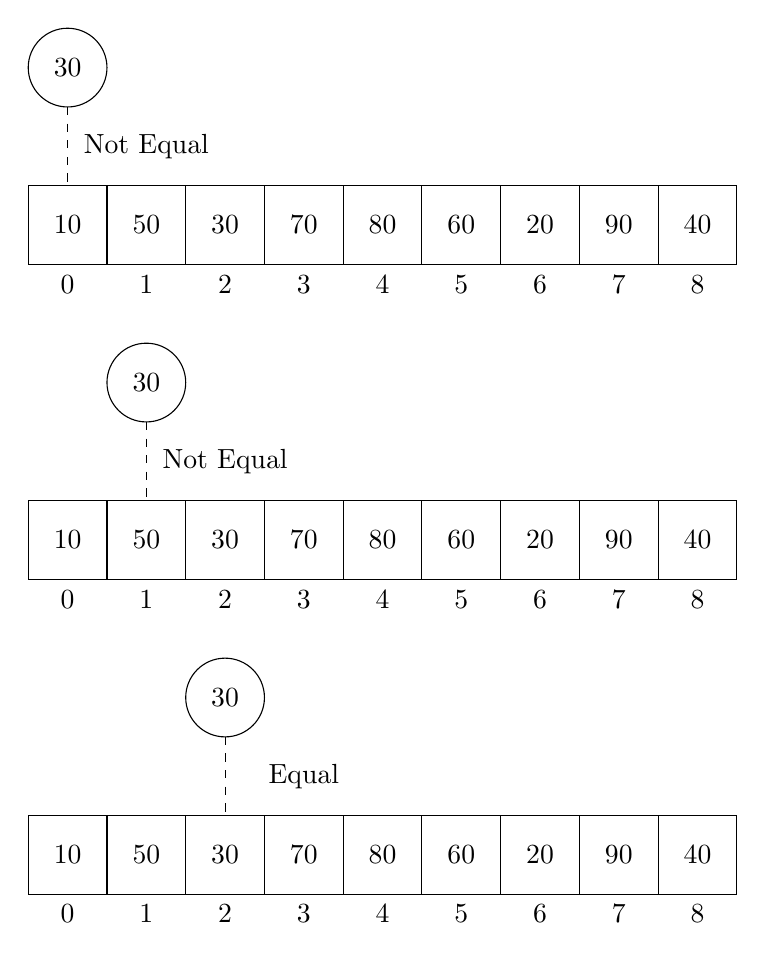
\begin{tikzpicture}
        % \node[fill=blue!30] (search) [box rounded] at (2, 4) {Search Element: 30};

        % 1st Element
        \draw (0.5, 2.5) circle (0.5);
        \node at (0.5, 2.5) {30};
        \draw[dashed] (0.5, 2) -- (0.5, 1);
        \node at (1.5, 1.5) {Not Equal};

        \draw (0, 0) rectangle (1, 1);
        \node at (0.5, 0.5) {10};
        \node at (0.5, -0.25) {0};
        \draw (1, 0) rectangle (2, 1);
        \node at (1.5, 0.5) {50};
        \node at (1.5, -0.25) {1};
        \draw (2, 0) rectangle (3, 1);
        \node at (2.5, 0.5) {30};
        \node at (2.5, -0.25) {2};
        \draw (3, 0) rectangle (4, 1);
        \node at (3.5, 0.5) {70};
        \node at (3.5, -0.25) {3};
        \draw (4, 0) rectangle (5, 1);
        \node at (4.5, 0.5) {80};
        \node at (4.5, -0.25) {4};
        \draw (5, 0) rectangle (6, 1);
        \node at (5.5, 0.5) {60};
        \node at (5.5, -0.25) {5};
        \draw (6, 0) rectangle (7, 1);
        \node at (6.5, 0.5) {20};
        \node at (6.5, -0.25) {6};
        \draw (7, 0) rectangle (8, 1);
        \node at (7.5, 0.5) {90};
        \node at (7.5, -0.25) {7};
        \draw (8, 0) rectangle (9, 1);
        \node at (8.5, 0.5) {40};
        \node at (8.5, -0.25) {8};

        % 2nd Element
        \draw (1.5, -1.5) circle (0.5);
        \node at (1.5, -1.5) {30};
        \draw[dashed] (1.5, -2) -- (1.5, -3);
        \node at (2.5, -2.5) {Not Equal};

        \draw (0, -4) rectangle (1, -3);
        \node at (0.5, -3.5) {10};
        \node at (0.5, -4.25) {0};
        \draw (1, -4) rectangle (2, -3);
        \node at (1.5, -3.5) {50};
        \node at (1.5, -4.25) {1};
        \draw (2, -4) rectangle (3, -3);
        \node at (2.5, -3.5) {30};
        \node at (2.5, -4.25) {2};
        \draw (3, -4) rectangle (4, -3);
        \node at (3.5, -3.5) {70};
        \node at (3.5, -4.25) {3};
        \draw (4, -4) rectangle (5, -3);
        \node at (4.5, -3.5) {80};
        \node at (4.5, -4.25) {4};
        \draw (5, -4) rectangle (6, -3);
        \node at (5.5, -3.5) {60};
        \node at (5.5, -4.25) {5};
        \draw (6, -4) rectangle (7, -3);
        \node at (6.5, -3.5) {20};
        \node at (6.5, -4.25) {6};
        \draw (7, -4) rectangle (8, -3);
        \node at (7.5, -3.5) {90};
        \node at (7.5, -4.25) {7};
        \draw (8, -4) rectangle (9, -3);
        \node at (8.5, -3.5) {40};
        \node at (8.5, -4.25) {8};

        % 3rd Element
        \draw (2.5, -5.5) circle (0.5);
        \node at (2.5, -5.5) {30};
        \draw[dashed] (2.5, -6) -- (2.5, -7);
        \node at (3.5, -6.5) {Equal};

        \draw (0, -8) rectangle (1, -7);
        \node at (0.5, -7.5) {10};
        \node at (0.5, -8.25) {0};
        \draw (1, -8) rectangle (2, -7);
        \node at (1.5, -7.5) {50};
        \node at (1.5, -8.25) {1};
        \draw (2, -8) rectangle (3, -7);
        \node at (2.5, -7.5) {30};
        \node at (2.5, -8.25) {2};
        \draw (3, -8) rectangle (4, -7);
        \node at (3.5, -7.5) {70};
        \node at (3.5, -8.25) {3};
        \draw (4, -8) rectangle (5, -7);
        \node at (4.5, -7.5) {80};
        \node at (4.5, -8.25) {4};
        \draw (5, -8) rectangle (6, -7);
        \node at (5.5, -7.5) {60};
        \node at (5.5, -8.25) {5};
        \draw (6, -8) rectangle (7, -7);
        \node at (6.5, -7.5) {20};
        \node at (6.5, -8.25) {6};
        \draw (7, -8) rectangle (8, -7);
        \node at (7.5, -7.5) {90};
        \node at (7.5, -8.25) {7};
        \draw (8, -8) rectangle (9, -7);
        \node at (8.5, -7.5) {40};
        \node at (8.5, -8.25) {8};

        % \node[fill=green!30] (search) [box rounded] at (2, -9.5) {30 Found at Index 2};
    \end{tikzpicture}
    \caption{Linear Search}
    \label{fig:linear-search}
\end{figure}

Figure \ref{fig:linear-search} shows the linear search algorithm in action.
The algorithm searches for the element 30 in an array of elements. It checks
each element one by one until it finds the desired element or reaches the end
of the array. In this case, the element 30 is found at index 2.

\subsubsection{Algorithm of Linear Search}

\begin{itemize}
    \item The Algorithm examines each element, one by one, in the 
    collection, treating each element as a potential match for the key 
    you’re searching for.

    \item The Algorithm examines each element, one by one, in the
    collection, treating each element as a potential match for the key
    you’re searching for.

    \item If it goes through all the elements and none of them matches
    the key, then that means “No match is Found”.
\end{itemize}

\subsubsection{Pseudo-code of Linear Search}

\begin{lstlisting}[caption={Linear Search Pseudo-code}]
LinearSearch(arr, key)
    for i = 0 to arr.length - 1
        if arr[i] == key
            return i
    return -1
\end{lstlisting}

Pseudo-code for Linear Search is shown in the code snippet. The algorithm
takes an array and a key as input and searches for the key in the array.
If the key is found, it returns the index of the key in the array; otherwise,
it returns -1.

\subsubsection{Linear Search in C++}

\begin{lstlisting}[language=C++, caption={Linear Search in C++}, label={lst:linear-search-cpp}]
#include <iostream>
#include <vector>
using namespace std;

int linearSearch(vector<int> &arr, int key) {
    int n = arr.size();
    for (int i = 0; i < n; i++) {
        if (arr[i] == key) {
            return i;
        }
    }
    return -1;
}

int main() {
    vector<int> arr = {10, 50, 30, 70, 80, 60, 20, 90, 40};
    int key = 30;

    int index = linearSearch(arr, key);

    if (index != -1) {
        cout << "Element found at index: " << index << endl;
    } else {
        cout << "Element not found" << endl;
    }

    return 0;
}
\end{lstlisting}

Code \ref{lst:linear-search-cpp} shows the implementation of the linear 
search algorithm in C++. The code snippet defines a function 
\texttt{linearSearch} that takes a vector of integers and a key as input
and searches for the key in the vector. If the key is found, it returns
the index of the key in the vector; otherwise, it returns -1. In the
example, the linear search algorithm is used to search for the element
30 in an array of elements. And the element is found at index 2.

\subsubsection{Application of Linear Search}

Linear search can be used in various applications, such as:

\begin{itemize}
    \item \textbf{Unsorted Lists}: Linear search is suitable for
    searching in unsorted lists where the elements are not in any
    particular order.

    \item \textbf{Small Data Sets}: Linear search is efficient for
    small data sets where the overhead of sorting the data is not
    justified.

    \item \textbf{Linear Data Structures}: Linear search is commonly
    used in linear data structures like arrays and linked lists as
    it traverses the elements sequentially.

    \item \textbf{Simple Search Operations}: Linear search is useful
    for simple search operations where the data is not too large and
    the search is infrequent.
\end{itemize}

\subsubsection{Advantages and Disadvantages of Linear Search}

\textbf{Advantages}:

\begin{itemize}
    \item Suitable for small data sets.
    \item Works well for unsorted lists.
    \item Does not require any additional memory.
\end{itemize}

\textbf{Disadvantages}:

\begin{itemize}
    \item Inefficient for large data sets as it has a time complexity
    of O(n) in the worst case.
    \item Not suitable for sorted lists.
    \item Slower than other searching algorithms like binary search.
\end{itemize}

\subsubsection{Complexity Analysis of Linear Search}

The time complexity of linear search is \texttt{O(n)}, where \texttt{n}
is the number of elements in the collection. In the worst-case scenario,
the algorithm may have to examine all elements in the collection to find
the desired element. The space complexity of linear search is \texttt{O(1)},
as it does not require any additional memory.

\subsection{Binary Search}

Binary search is a searching algorithm that finds the position of a target
value within a sorted array. It compares the target value to the middle element
of the array and eliminates half of the remaining elements each time. Binary
search is more efficient than linear search for large data sets.

% TikZ Figure for Binary Search
\begin{figure}[h!]
    \centering
    \begin{tikzpicture}
        % Initial
        \node[text width=4cm] (search) [box rounded] at (-3, 0.5) {Search Element: 23};

        \draw (0, 0) rectangle (1, 1);
        \node at (0.5, 0.5) {2};
        \node at (0.5, -0.25) {0};
        \draw (1, 0) rectangle (2, 1);
        \node at (1.5, 0.5) {5};
        \node at (1.5, -0.25) {1};
        \draw (2, 0) rectangle (3, 1);
        \node at (2.5, 0.5) {8};
        \node at (2.5, -0.25) {2};
        \draw (3, 0) rectangle (4, 1);
        \node at (3.5, 0.5) {12};
        \node at (3.5, -0.25) {3};
        \draw (4, 0) rectangle (5, 1);
        \node at (4.5, 0.5) {16};
        \node at (4.5, -0.25) {4};
        \draw (5, 0) rectangle (6, 1);
        \node at (5.5, 0.5) {23};
        \node at (5.5, -0.25) {5};
        \draw (6, 0) rectangle (7, 1);
        \node at (6.5, 0.5) {38};
        \node at (6.5, -0.25) {6};
        \draw (7, 0) rectangle (8, 1);
        \node at (7.5, 0.5) {56};
        \node at (7.5, -0.25) {7};
        \draw (8, 0) rectangle (9, 1);
        \node at (8.5, 0.5) {72};
        \node at (8.5, -0.25) {8};
        \draw (9, 0) rectangle (10, 1);
        \node at (9.5, 0.5) {91};
        \node at (9.5, -0.25) {9};
        
        % 1st Iteration
        \node[text width=4cm] (mid1) [box rounded] at (-3, -1.5) {
            23 > 16, take 2nd half
        };
        
        \draw (0, -2) rectangle (1, -1);
        \node at (0.5, -1.5) {2};
        \node[text=blue] at (0.5, -2.25) {L=0};
        \draw (1, -2) rectangle (2, -1);
        \node at (1.5, -1.5) {5};
        \node at (1.5, -2.25) {1};
        \draw (2, -2) rectangle (3, -1);
        \node at (2.5, -1.5) {8};
        \node at (2.5, -2.25) {2};
        \draw (3, -2) rectangle (4, -1);
        \node at (3.5, -1.5) {12};
        \node at (3.5, -2.25) {3};
        \draw[fill=green!30] (4, -2) rectangle (5, -1);
        \node at (4.5, -1.5) {16};
        \node[text=black!20!green] at (4.5, -2.25) {M=4};
        \draw (5, -2) rectangle (6, -1);
        \node at (5.5, -1.5) {23};
        \node at (5.5, -2.25) {5};
        \draw (6, -2) rectangle (7, -1);
        \node at (6.5, -1.5) {38};
        \node at (6.5, -2.25) {6};
        \draw (7, -2) rectangle (8, -1);
        \node at (7.5, -1.5) {56};
        \node at (7.5, -2.25) {7};
        \draw (8, -2) rectangle (9, -1);
        \node at (8.5, -1.5) {72};
        \node at (8.5, -2.25) {8};
        \draw (9, -2) rectangle (10, -1);
        \node at (9.5, -1.5) {91};
        \node[text=red] at (9.5, -2.25) {H=9};

        % 2nd Iteration
        \node[text width=4cm] (mid2) [box rounded] at (-3, -3.5) {
            23 < 56, take 1st half
        };

        \draw[fill=gray!30] (0, -4) rectangle (1, -3);
        \node at (0.5, -3.5) {2};
        \node at (0.5, -4.25) {0};
        \draw[fill=gray!30] (1, -4) rectangle (2, -3);
        \node at (1.5, -3.5) {5};
        \node at (1.5, -4.25) {1};
        \draw[fill=gray!30] (2, -4) rectangle (3, -3);
        \node at (2.5, -3.5) {8};
        \node at (2.5, -4.25) {2};
        \draw[fill=gray!30] (3, -4) rectangle (4, -3);
        \node at (3.5, -3.5) {12};
        \node at (3.5, -4.25) {3};
        \draw[fill=gray!30] (4, -4) rectangle (5, -3);
        \node at (4.5, -3.5) {16};
        \node at (4.5, -4.25) {4};
        \draw (5, -4) rectangle (6, -3);
        \node at (5.5, -3.5) {23};
        \node[text=blue] at (5.5, -4.25) {L=5};
        \draw (6, -4) rectangle (7, -3);
        \node at (6.5, -3.5) {38};
        \node at (6.5, -4.25) {6};
        \draw[fill=green!30] (7, -4) rectangle (8, -3);
        \node at (7.5, -3.5) {56};
        \node[text=black!20!green] at (7.5, -4.25) {M=7};
        \draw (8, -4) rectangle (9, -3);
        \node at (8.5, -3.5) {72};
        \node at (8.5, -4.25) {8};
        \draw (9, -4) rectangle (10, -3);
        \node at (9.5, -3.5) {91};
        \node[text=red] at (9.5, -4.25) {H=9};

        % 3rd Iteration
        \node[text width=4cm] (mid3) [box rounded] at (-3, -5.5) {
            Found 23, Return 5
        };

        \draw[fill=gray!30] (0, -6) rectangle (1, -5);
        \node at (0.5, -5.5) {2};
        \node at (0.5, -6.25) {0};
        \draw[fill=gray!30] (1, -6) rectangle (2, -5);
        \node at (1.5, -5.5) {5};
        \node at (1.5, -6.25) {1};
        \draw[fill=gray!30] (2, -6) rectangle (3, -5);
        \node at (2.5, -5.5) {8};
        \node at (2.5, -6.25) {2};
        \draw[fill=gray!30] (3, -6) rectangle (4, -5);
        \node at (3.5, -5.5) {12};
        \node at (3.5, -6.25) {3};
        \draw[fill=gray!30] (4, -6) rectangle (5, -5);
        \node at (4.5, -5.5) {16};
        \node at (4.5, -6.25) {4};
        \draw[fill=green!30] (5, -6) rectangle (6, -5);
        \node at (5.5, -5.5) {23};
        \node[text=blue] at (5.5, -6.25) {L=5};
        \node[text=black!20!green] at (5.5, -6.75) {M=5};
        \draw (6, -6) rectangle (7, -5);
        \node at (6.5, -5.5) {38};
        \node[text=red] at (6.5, -6.25) {H=6};
        \draw[fill=gray!30] (7, -6) rectangle (8, -5);
        \node at (7.5, -5.5) {56};
        \node at (7.5, -6.25) {7};
        \draw[fill=gray!30] (8, -6) rectangle (9, -5);
        \node at (8.5, -5.5) {72};
        \node at (8.5, -6.25) {8};
        \draw[fill=gray!30] (9, -6) rectangle (10, -5);
        \node at (9.5, -5.5) {91};
        \node at (9.5, -6.25) {9};
    \end{tikzpicture}
    \caption{Binary Search}
    \label{fig:binary-search}    
\end{figure}

Figure \ref{fig:binary-search} shows the binary search algorithm in 
action. The algorithm searches for the element 23 in a sorted array
of elements. It compares the target value to the middle element of
the array and eliminates half of the remaining elements each time.
In the 1st iteration, the algorithm compares 23 with 16 and decides
to take the 2nd half since 23 > 16. In the 2nd iteration, the algorithm
compares 23 with 56 and decides to take the 1st half since 23 < 56.
In the 3rd iteration, the algorithm finds 23 at index 5 and returns
the index.

\subsubsection{Algorithm of Binary Search}

\begin{itemize}
    \item Divide the search space into two halves by finding the 
    middle index ``mid''.

    \item Compare the middle element of the search space with the key.
    
    \item Compare the middle element of the search space with the key.

    \item If the key is not found at middle element, choose which
    half will be used as the next search space.
    \begin{itemize}
        \item If the key is not found at middle element, choose which
        half will be used as the next search space.
        
        \item If the key is not found at middle element, choose which
        half will be used as the next search space.
    \end{itemize}

    \item If the key is not found at middle element, choose which half
    will be used as the next search space.
\end{itemize}

\subsubsection{Pseudo-code of Binary Search}

\begin{lstlisting}[caption={Binary Search Pseudo-code}]
BinarySearch(arr, key)
    low = 0
    high = arr.length - 1
    while low <= high
        mid = low + (low + high) / 2
        if arr[mid] == key
            return mid
        else if arr[mid] < key
            low = mid + 1
        else
            high = mid - 1
    return -1
\end{lstlisting}

Pseudo-code for Binary Search is shown in the code snippet. The algorithm
takes a sorted array and a key as input and searches for the key in the
array using the binary search technique. If the key is found, it returns
the index of the key in the array; otherwise, it returns -1.

\subsubsection{Binary Search in C++}

\begin{lstlisting}[language=C++, caption={Binary Search in C++}, label={lst:binary-search-cpp}]
#include <iostream>
#include <vector>
using namespace std;

int binarySearch(vector<int> &arr, int key) {
    int low = 0;
    int high = arr.size() - 1;

    while (low <= high) {
        int mid = low + (high - low) / 2;

        if (arr[mid] == key) {
            return mid;
        } else if (arr[mid] < key) {
            low = mid + 1;
        } else {
            high = mid - 1;
        }
    }

    return -1;
}

int main() {
    vector<int> arr = {2, 5, 8, 12, 16, 23, 38, 56, 72, 91};
    int key = 23;

    int index = binarySearch(arr, key);

    if (index != -1) {
        cout << "Element found at index: " << index << endl;
    } else {
        cout << "Element not found" << endl;
    }

    return 0;
}
\end{lstlisting}

Code \ref{lst:binary-search-cpp} shows the implementation of the binary
search algorithm in C++. The code snippet defines a function
\texttt{binarySearch} that takes a vector of integers and a key as input
and searches for the key in the vector using the binary search technique.
If the key is found, it returns the index of the key in the vector;
otherwise, it returns -1. In the example, the binary search algorithm is
used to search for the element 23 in a sorted array of elements. And the
element is found at index 5. During the search process, the algorithm
compares the target value to the middle element of the array and eliminates
half of the remaining elements each time. If the middle element is greater
than the target value, the algorithm chooses the 1st half as the next search
space; otherwise, it chooses the 2nd half. For each iteration, the algorithm
updates the low and high indices to narrow down the search space until the
target value is found or the search space is empty. If the search space is
empty, the algorithm returns -1 to indicate that the target value is not
present in the array.

\subsubsection{Application of Binary Search}

Binary search can be used in various applications, such as:

\begin{itemize}
    \item \textbf{Building Block}: Binary search can be used as a 
    building block for more complex algorithms used in machine 
    learning, such as algorithms for training neural networks or 
    finding the optimal hyperparameters for a model.
    
    \item \textbf{Computer Graphics}: It can be used for searching 
    in computer graphics such as algorithms for ray tracing or 
    texture mapping.
    
    \item \textbf{Database}: It can be used for searching a database.
\end{itemize}

\subsubsection{Advantages and Disadvantages of Binary Search}

\textbf{Advantages}:

\begin{itemize}
    \item More efficient than linear search for large data sets.
    
    \item More efficient than other searching algorithms with a 
    similar time complexity, such as interpolation search or 
    exponential search.
    
    \item Binary search is well-suited for searching large datasets 
    that are stored in external memory, such as on a hard drive or 
    in the cloud.
\end{itemize}

\textbf{Disadvantages}:

\begin{itemize}
    \item The array should be sorted.
    \item Binary search requires that the data structure being
    searched be stored in contiguous memory locations. 
    \item Binary search requires that the elements of the array be 
    comparable, meaning that they must be able to be ordered.
\end{itemize}

\subsubsection{Complexity Analysis of Binary Search}

The time complexity of binary search is \texttt{O(log n)}, where 
\texttt{n} is the number of elements in the collection. In each
iteration, the search space is divided in half, resulting in a
time complexity of \texttt{O(log n)}. The space complexity of
binary search is \texttt{O(1)}, as it does not require any
additional memory.

\subsection{Other Searching Algorithms}

Apart from linear search and binary search, there are several other
searching algorithms that are commonly used in practice. Some of the
popular searching algorithms are:

\begin{itemize}
    \item \textbf{Jump Search}: Jump search is an algorithm for finding
    the position of a target value within a sorted array. It works by
    jumping ahead by fixed steps and then performing a linear search
    to find the target value.
    
    \item \textbf{Interpolation Search}: Interpolation search is an
    algorithm for finding the position of a target value within a sorted
    array. It works by estimating the position of the target value based
    on the values at the ends of the array and then performing a binary
    search to find the target value.
    
    \item \textbf{Exponential Search}: Exponential search is an algorithm
    for finding the position of a target value within a sorted array. It
    works by doubling the size of the search space until the target value
    is found, and then performing a binary search to find the target value.
    
    \item \textbf{Fibonacci Search}: Fibonacci search is an algorithm for
    finding the position of a target value within a sorted array. It works
    by dividing the search space into two parts using the Fibonacci numbers
    and then performing a binary search to find the target value.
    
    \item \textbf{Hash Search}: Hash search is an algorithm for finding the
    position of a target value within a hash table. It works by using a hash
    function to map the target value to a key and then looking up the key in
    the hash table to find the target value.
\end{itemize}

\section{Summary}

In this chapter, we discussed the searching algorithms, especially the
linear search and binary search algorithms. We explained the working
principles of these algorithms, provided pseudo-code examples, and
implemented them in C++. We also discussed the applications, advantages,
disadvantages, and complexity analysis of these algorithms. Additionally,
we introduced other searching algorithms such as jump search, interpolation
search, exponential search, Fibonacci search, and hash search. These
searching algorithms play a crucial role in various applications and are
essential building blocks for more complex algorithms used in computer
science and related fields.

%%%%%%%%%%%%%%%%%%%%%%%%%%%%%%%%%%%%
%%%%%~ NEW CHAPTER STARTS HERE %%%%%
%%%%%%%%%%%%%%%%%%%%%%%%%%%%%%%%%%%%

\chapter{Sorting Algorithms}

\section{Introduction}

Imagine you have a messy pile of socks, and you want to organize them 
by color. That's exactly what a sorting algorithm does, but with data! 
Sorting algorithms are fundamental techniques used to arrange the 
elements of a data structure in a specific order, such as ascending or 
descending. These algorithms are crucial in computer science because 
they optimize the efficiency of other algorithms that require sorted 
data, like search algorithms. Whether it's Bubble Sort gently swapping 
elements  like a careful librarian, or Quick Sort slicing through data 
like a  ninja chef, these algorithms make sure everything is in the 
right  place. And the best part? Most programming languages come with 
these  sorting Algorithms built-in, so you don't have to reinvent the 
wheel  every time you need to sort something.

\section{Importance of Sorting Algorithms}

Sorting algorithms are essential in computer science and programming
as they are used to arrange data in a specific order. There is a wide 
range of applications for these algorithms, including searching 
algorithms, database algorithms, divide and conquer methods, and data 
structure algorithms. Here are some of the key reasons why sorting
algorithms are important:

\begin{itemize}
    \item \textbf{Efficient Searching}: Sorting algorithms are used to
    arrange data in a specific order, making it easier and faster to
    search for elements in the data structure. For example, binary
    search requires the data to be sorted before it can be applied.
    
    \item \textbf{Data Analysis}: Sorting algorithms are used in data
    analysis to organize and analyze large datasets. By sorting the
    data, patterns and trends can be identified more easily.
    
    \item \textbf{Database Management}: Sorting algorithms are used in
    database management systems to sort records and improve the
    efficiency of queries and data retrieval.
    
    \item \textbf{Optimization}: Sorting algorithms are used in
    optimization problems to arrange elements in a specific order
    that minimizes or maximizes a certain criterion.
    
    \item \textbf{Data Structure Operations}: Sorting algorithms are
    used in various data structure operations, such as merging two
    sorted arrays, finding the median of a dataset, and removing
    duplicates from a list.

    \item \textbf{Machine Learning}: Sorting algorithms are used in
    machine learning algorithms to preprocess and organize data
    before training models. Sorting data can improve the performance
    of machine learning algorithms and make them more efficient.

    \item \textbf{Operating Systems}: Sorting algorithms are used in
    operating systems to manage and organize files and directories.
    By sorting files and directories, the user can easily locate and
    access the required information.
\end{itemize}

\section{Types of Sorting Techniques}

There are various sorting algorithms are used in data structures. 
The following two types of sorting algorithms can be broadly 
classified:

\begin{enumerate}
    \item \textbf{Comparison-based Sorting Algorithms}: In comparison-based
    sorting algorithms, elements are compared with each other to determine
    their relative order. The most common comparison-based sorting algorithms
    include Bubble Sort, Selection Sort, Insertion Sort, Merge Sort, Quick
    Sort, and Heap Sort.

    \item \textbf{Non-comparison-based Sorting Algorithms}: In non-comparison-based
    sorting algorithms, elements are not compared with each other directly.
    Instead, these algorithms use specific properties of the elements to
    determine their order. The most common non-comparison-based sorting
\end{enumerate}

\begin{figure}[h!]
    \centering
    \begin{tikzpicture}[
        every node/.style={rectangle, fill=white, draw, align=center}
    ]
        % Nodes
        \node (sorting) {Sorting Algorithms};
        
        \node (comparison) [below left=of sorting] {Comparison-Based};
        \node (noncomparison) [below right=of sorting] {Non-comparison-Based};
        
        \node (bubble) [below=of comparison] {Bubble Sort};
        \node (selection) [below=of bubble] {Selection Sort};
        \node (insertion) [below=of selection] {Insertion Sort};
        \node (merge) [below=of insertion] {Merge Sort};
        \node (quick) [below=of merge] {Quick Sort};
        \node (heap) [below=of quick] {Heap Sort};
        \node (left end) [below=of heap] {};
        \node (counting) [below=of noncomparison] {Counting Sort};
        \node (radix) [below=of counting] {Radix Sort};
        \node (right end) [below=of radix] {};

        % Edges
        \begin{scope}[on background layer]
            \draw[->] (sorting) -- (comparison);
            \draw[->] (sorting) -- (noncomparison);

            \draw[-] (comparison) -- (bubble);
            \draw[-] (comparison) -- (selection);
            \draw[-] (comparison) -- (insertion);
            \draw[-] (comparison) -- (merge);
            \draw[-] (comparison) -- (quick);
            \draw[-] (comparison) -- (heap);
            \draw[-] (comparison) -- (left end);
            
            \draw[-] (noncomparison) -- (counting);
            \draw[-] (noncomparison) -- (radix);
            \draw[-] (noncomparison) -- (right end);
        \end{scope}
    \end{tikzpicture}
    \caption{Sorting Techniques}
    \label{fig:sorting-techniques}
\end{figure}

\section{Types of Comparison-Based Sorting Algorithms}

There are various types of sorting algorithms used in computer science
and programming. These sorting algorithms can be broadly classified
into two categories: comparison-based sorting algorithms and
non-comparison-based sorting algorithms.

\subsection{Selection Sort}

Selection Sort is a simple sorting algorithm that works by repeatedly
selecting the minimum element from the unsorted portion of the array
and swapping it with the first unsorted element. The algorithm divides
the array into two parts: the sorted part at the beginning and the
unsorted part at the end. In each iteration, the algorithm finds the
minimum element in the unsorted part and swaps it with the first
unsorted element. This process continues until the entire array is
sorted.

% Create a TikzPicture
\begin{figure}[h!]
    \centering
    \begin{tikzpicture}
        % 1st Swap
        \node[text width=5cm] (search) [box rounded] at (-4, 0.5) {
            Current is 64, Minimum is 11, SWAP
        };

        \draw (0, 0) rectangle (1, 1);
        \node at (0.5, 0.5) {64};
        \node at (0.5, -0.25) {0};
        \draw (1, 0) rectangle (2, 1);
        \node at (1.5, 0.5) {25};
        \node at (1.5, -0.25) {1};
        \draw (2, 0) rectangle (3, 1);
        \node at (2.5, 0.5) {12};
        \node at (2.5, -0.25) {2};
        \draw (3, 0) rectangle (4, 1);
        \node at (3.5, 0.5) {22};
        \node at (3.5, -0.25) {3};
        \draw (4, 0) rectangle (5, 1);
        \node at (4.5, 0.5) {11};
        \node at (4.5, -0.25) {4};

        % Curved Arrow From 0 to 4 and vice-versa
        \draw[->, bend left=45] (0.5, 1) to (4.5, 1);
        \draw[->, bend left=-45] (4.5, 1) to (0.5, 1);
        \node at (2.5, 2.125) {Swap 64 and 11};

        % 2nd Swap
        \node[text width=5cm] (search) [box rounded] at (-4, -2.5) {
            Current is 25, Minimum is 12, SWAP
        };

        \draw[fill=green!30] (0, -3) rectangle (1, -2); %SORTED
        \node at (0.5, -2.5) {11};
        \node at (0.5, -3.25) {0};
        \draw (1, -3) rectangle (2, -2);
        \node at (1.5, -2.5) {25};
        \node at (1.5, -3.25) {1};
        \draw (2, -3) rectangle (3, -2);
        \node at (2.5, -2.5) {12};
        \node at (2.5, -3.25) {2};
        \draw (3, -3) rectangle (4, -2);
        \node at (3.5, -2.5) {22};
        \node at (3.5, -3.25) {3};
        \draw (4, -3) rectangle (5, -2);
        \node at (4.5, -2.5) {64};
        \node at (4.5, -3.25) {4};

        % Curved Arrow From 1 to 2 and vice-versa
        \draw[->, bend left=45] (1.5, -2) to (2.5, -2);
        \draw[->, bend left=-45] (2.5, -2) to (1.5, -2);
        \node at (2, -1.5) {Swap 25 and 12};

        % 3rd Swap
        \node[text width=5cm] (search) [box rounded] at (-4, -5.5) {
            Current is 22, Minimum is 12, SWAP
        };

        \draw[fill=green!30] (0, -6) rectangle (1, -5); %SORTED
        \node at (0.5, -5.5) {11};
        \node at (0.5, -6.25) {0};
        \draw[fill=green!30] (1, -6) rectangle (2, -5); %SORTED
        \node at (1.5, -5.5) {12};
        \node at (1.5, -6.25) {1};
        \draw (2, -6) rectangle (3, -5);
        \node at (2.5, -5.5) {25};
        \node at (2.5, -6.25) {2};
        \draw (3, -6) rectangle (4, -5);
        \node at (3.5, -5.5) {22};
        \node at (3.5, -6.25) {3};
        \draw (4, -6) rectangle (5, -5);
        \node at (4.5, -5.5) {64};
        \node at (4.5, -6.25) {4};
        
        % Curved Arrow From 2 to 3 and vice-versa
        \draw[->, bend left=45] (2.5, -5) to (3.5, -5);
        \draw[->, bend left=-45] (3.5, -5) to (2.5, -5);
        \node at (3, -4.5) {Swap 25 and 22};

        % 4th Swap
        \node[text width=5cm] (search) [box rounded] at (-4, -8.5) {
            Current is 25, Minimum is 25, NO SWAP
        };

        \draw[fill=green!30] (0, -9) rectangle (1, -8); %SORTED
        \node at (0.5, -8.5) {11};
        \node at (0.5, -9.25) {0};
        \draw[fill=green!30] (1, -9) rectangle (2, -8); %SORTED
        \node at (1.5, -8.5) {12};
        \node at (1.5, -9.25) {1};
        \draw[fill=green!30] (2, -9) rectangle (3, -8); %SORTED
        \node at (2.5, -8.5) {22};
        \node at (2.5, -9.25) {2};
        \draw (3, -9) rectangle (4, -8);
        \node at (3.5, -8.5) {25};
        \node at (3.5, -9.25) {3};
        \draw (4, -9) rectangle (5, -8);
        \node at (4.5, -8.5) {64};
        \node at (4.5, -9.25) {4};

        %  5th Swap
        \node[text width=5cm] (search) [box rounded] at (-4, -11.5) {
            Current is 64, Minimum is 64, NO SWAP
        };

        \draw[fill=green!30] (0, -12) rectangle (1, -11); %SORTED
        \node at (0.5, -11.5) {11};
        \node at (0.5, -12.25) {0};
        \draw[fill=green!30] (1, -12) rectangle (2, -11); %SORTED
        \node at (1.5, -11.5) {12};
        \node at (1.5, -12.25) {1};
        \draw[fill=green!30] (2, -12) rectangle (3, -11); %SORTED
        \node at (2.5, -11.5) {22};
        \node at (2.5, -12.25) {2};
        \draw[fill=green!30] (3, -12) rectangle (4, -11); %SORTED
        \node at (3.5, -11.5) {25};
        \node at (3.5, -12.25) {3};
        \draw (4, -12) rectangle (5, -11);
        \node at (4.5, -11.5) {64};
        \node at (4.5, -12.25) {4};
        
        % Final
        \node[text width=5cm] (search) [box rounded] at (-4, -14.5) {
            Sorted Array: 11, 12, 22, 25, 64
        };

        \draw[fill=green!30] (0, -15) rectangle (1, -14); %SORTED
        \node at (0.5, -14.5) {11};
        \node at (0.5, -15.25) {0};
        \draw[fill=green!30] (1, -15) rectangle (2, -14); %SORTED
        \node at (1.5, -14.5) {12};
        \node at (1.5, -15.25) {1};
        \draw[fill=green!30] (2, -15) rectangle (3, -14); %SORTED
        \node at (2.5, -14.5) {22};
        \node at (2.5, -15.25) {2};
        \draw[fill=green!30] (3, -15) rectangle (4, -14); %SORTED
        \node at (3.5, -14.5) {25};
        \node at (3.5, -15.25) {3};
        \draw[fill=green!30] (4, -15) rectangle (5, -14); %SORTED
        \node at (4.5, -14.5) {64};
        \node at (4.5, -15.25) {4};
    \end{tikzpicture}
    \caption{Selection Sort}
    \label{fig:selection-sort}
\end{figure}

Figure \ref{fig:selection-sort} shows the Selection Sort algorithm in
action. The algorithm sorts an array of elements by repeatedly selecting
the minimum element from the unsorted portion of the array and swapping
it with the first unsorted element. In each iteration, the algorithm
finds the minimum element in the unsorted part and swaps it with the
first unsorted element. This process continues until the entire array
is sorted.

\subsubsection{Algorithm of Selection Sort}

\begin{itemize}
    \item Divide the array into two parts: the sorted part at the
    beginning and the unsorted part at the end.
    
    \item Find the minimum element in the unsorted part of the array.
    
    \item Swap the minimum element with the first unsorted element.
    
    \item Repeat the process for the remaining unsorted elements until
    the entire array is sorted.
\end{itemize}

\subsubsection{Pseudo-code of Selection Sort}

\begin{lstlisting}[caption={Selection Sort Pseudo-code}]
SelectionSort(arr)
    n = arr.length
    for i = 0 to n-2
        minIndex = i
        for j = i+1 to n - 1
            if arr[j] < arr[minIndex]
                minIndex = j
        swap(arr[i], arr[minIndex])
\end{lstlisting}

Pseudo-code for Selection Sort is shown in the code snippet. The algorithm
takes an array of elements as input and sorts the array using the Selection
Sort technique. The algorithm iterates through the array, finds the minimum
element in the unsorted part, and swaps it with the first unsorted element.
This process continues until the entire array is sorted.

\subsubsection{Selection Sort in C++}

\begin{lstlisting}[language=C++, caption={Selection Sort in C++}, label={lst:selection-sort-cpp}]
#include <iostream>
#include <vector>
using namespace std;

void selectionSort(vector<int> &arr) {
    int n = arr.size();

    for (int i = 0; i < n - 1; i++) {
        int minIndex = i;

        for (int j = i + 1; j < n; j++) {
            if (arr[j] < arr[minIndex]) {
                minIndex = j;
            }
        }

        swap(arr[i], arr[minIndex]);
    }
}

void printArray(vector<int> &arr) {
    for (int i = 0; i < arr.size(); i++) {
        cout << arr[i] << " ";
    }
    cout << endl;
}

int main() {
    vector<int> arr = {64, 25, 12, 22, 11};
    
    cout << "Original Array: ";
    printArray(arr);

    selectionSort(arr);

    cout << "Sorted Array: ";
    printArray(arr);

    return 0;
}
\end{lstlisting}

Code \ref{lst:selection-sort-cpp} shows the implementation of the Selection
Sort algorithm in C++. The code snippet defines a function \texttt{selectionSort}
that takes a vector of integers as input and sorts the array using the Selection
Sort technique. The algorithm iterates through the array, finds the minimum element
in the unsorted part, and swaps it with the first unsorted element. This process
continues until the entire array is sorted. In the example, the Selection Sort
algorithm is used to sort an array of elements, and the sorted array is printed
to the console.

% \subsubsection{Application of Selection Sort}

% \begin{itemize}
%     \item \textbf{Teaching}: Selection Sort is often used in computer science
%     courses to teach fundamental sorting mechanisms and algorithm design.
    
%     \item \textbf{Small Lists}: Selection Sort is suitable for small lists
%     where the overhead of more complex algorithms isn't justified.
    
%     \item \textbf{Limited Memory}: Selection Sort is ideal for systems with
%     limited memory due to its in-place sorting capability.
    
%     \item \textbf{Embedded Systems}: Selection Sort is used in simple embedded
%     systems where resource availability is limited, and simplicity is important.
% \end{itemize}

\subsubsection{Advantages and Disadvantages of Selection Sort}

\textbf{Advantages}:

\begin{itemize}
    \item Easy to understand and implement, making it ideal for teaching
    basic sorting concepts.
    
    \item Requires only a constant \texttt{$O(1)$} extra memory space.
    
    \item Requires less number of swaps (or memory writes) compared to
    many other standard algorithms. Only cycle sort beats it in terms
    of memory writes. Therefore, it can be a simple algorithm choice
    when memory writes are costly.
\end{itemize}

\textbf{Disadvantages}:

\begin{itemize}
    \item Selection sort has a time complexity of \texttt{$O(n^2)$} makes
    it slower compared to algorithms like Quick Sort or Merge Sort.
    
    \item Does not maintain the relative order of equal elements.
    
    \item Does not preserve the relative order of items with equal keys
    which means it is not stable.
\end{itemize}

\subsubsection{Complexity Analysis of Selection Sort}

The time complexity of Selection Sort is \texttt{$O(n^2)$}, where
\texttt{$n$} is the number of elements in the array. The space
complexity of Selection Sort is \texttt{$O(1)$}, as it does not
require any additional memory.

\subsection{Bubble Sort}

Bubble Sort is a simple sorting algorithm that repeatedly steps through
the list, compares adjacent elements, and swaps them if they are in the
wrong order. For each pass through the list, the largest element goes
to the end of the list. If a larger element is found, it is swapped with
the next element, and the process is repeated until the list is sorted.

% Create a TikzPicture
\begin{figure}[h!]
    \centering
    \begin{tikzpicture}
        % 1st Iteration
        % 1st Swap
        \node at (2, 4.5) {
            Initial Array: 5, 6, 1, 3
        };

        \node[text width=5cm] (search) [box rounded] at (-4, 3) {
            Current is 5: 5 < 6, NO SWAP
        };

        \draw (0, 2.5) rectangle (1, 3.5);
        \node at (0.5, 3) {5};
        \node at (0.5, 2.25) {0};
        \draw (1, 2.5) rectangle (2, 3.5);
        \node at (1.5, 3) {6};
        \node at (1.5, 2.25) {1};
        \draw (2, 2.5) rectangle (3, 3.5);
        \node at (2.5, 3) {1};
        \node at (2.5, 2.25) {2};
        \draw (3, 2.5) rectangle (4, 3.5);
        \node at (3.5, 3) {3};
        \node at (3.5, 2.25) {3};

        % 2nd Swap
        \node[text width=5cm] (search) [box rounded] at (-4, 0.5) {
            Current is 6; 6 > 1, SWAP
        };

        \draw (0, 0) rectangle (1, 1);
        \node at (0.5, 0.5) {5};
        \node at (0.5, -0.25) {0};
        \draw (1, 0) rectangle (2, 1);
        \node at (1.5, 0.5) {6};
        \node at (1.5, -0.25) {1};
        \draw (2, 0) rectangle (3, 1);
        \node at (2.5, 0.5) {1};
        \node at (2.5, -0.25) {2};
        \draw (3, 0) rectangle (4, 1);
        \node at (3.5, 0.5) {3};
        \node at (3.5, -0.25) {3};

        % Curved Arrow From 1 to 2 and vice-versa
        \draw[->, bend left=45] (1.5, 1) to (2.5, 1);
        \draw[->, bend left=-45] (2.5, 1) to (1.5, 1);
        \node at (2, 1.5) {Swap 6 and 1};

        % 3rd Swap
        \node[text width=5cm] (search) [box rounded] at (-4, -2) {
            Current is 6; 6 > 3, SWAP
        };

        \draw (0, -2.5) rectangle (1, -1.5);
        \node at (0.5, -2) {5};
        \node at (0.5, -2.75) {0};
        \draw (1, -2.5) rectangle (2, -1.5);
        \node at (1.5, -2) {1};
        \node at (1.5, -2.75) {1};
        \draw (2, -2.5) rectangle (3, -1.5);
        \node at (2.5, -2) {6};
        \node at (2.5, -2.75) {2};
        \draw (3, -2.5) rectangle (4, -1.5);
        \node at (3.5, -2) {3};
        \node at (3.5, -2.75) {3};

        % Curved Arrow From 2 to 3 and vice-versa
        \draw[->, bend left=45] (2.5, -1.5) to (3.5, -1.5);
        \draw[->, bend left=-45] (3.5, -1.5) to (2.5, -1.5);
        \node at (3, -1) {Swap 6 and 3};

        % Final during 1st Iteration
        \node[text width=5cm] (search) [box rounded] at (-4, -4.5) {
            5, 1, 3, 6
        };

        \node[text width=4cm] (search) [box rounded] at (7, -4.5) {
            Sorted: 6
        };

        \draw (0, -5) rectangle (1, -4);
        \node at (0.5, -4.5) {5};
        \node at (0.5, -5.25) {0};
        \draw (1, -5) rectangle (2, -4);
        \node at (1.5, -4.5) {1};
        \node at (1.5, -5.25) {1};
        \draw (2, -5) rectangle (3, -4);
        \node at (2.5, -4.5) {3};
        \node at (2.5, -5.25) {2};
        \draw[fill=green!30] (3, -5) rectangle (4, -4);
        \node at (3.5, -4.5) {6};
        \node at (3.5, -5.25) {3};

        % 2nd Iteration
        % 1st Swap
        \node[text width=5cm] (search) [box rounded] at (-4, -7) {
            Current is 5; 5 > 1, SWAP
        };

        \draw (0, -7.5) rectangle (1, -6.5);
        \node at (0.5, -7) {5};
        \node at (0.5, -7.75) {0};
        \draw (1, -7.5) rectangle (2, -6.5);
        \node at (1.5, -7) {1};
        \node at (1.5, -7.75) {1};
        \draw (2, -7.5) rectangle (3, -6.5);
        \node at (2.5, -7) {3};
        \node at (2.5, -7.75) {2};
        \draw[fill=green!30] (3, -7.5) rectangle (4, -6.5);
        \node at (3.5, -7) {6};
        \node at (3.5, -7.75) {3};

        % Curved Arrow From 0 to 1
        \draw[->, bend left=45] (0.5, -6.5) to (1.5, -6.5);
        \draw[->, bend left=-45] (1.5, -6.5) to (0.5, -6.5);
        \node at (1, -6) {Swap 5 and 1};

        % 2nd Swap
        \node[text width=5cm] (search) [box rounded] at (-4, -9.5) {
            Current is 5; 5 > 3, SWAP
        };
        \draw (0, -10) rectangle (1, -9);
        \node at (0.5, -9.5) {1};
        \node at (0.5, -10.25) {0};
        \draw (1, -10) rectangle (2, -9);
        \node at (1.5, -9.5) {5};
        \node at (1.5, -10.25) {1};
        \draw (2, -10) rectangle (3, -9);
        \node at (2.5, -9.5) {3};
        \node at (2.5, -10.25) {2};
        \draw[fill=green!30] (3, -10) rectangle (4, -9);
        \node at (3.5, -9.5) {6};
        \node at (3.5, -10.25) {3};

        % Curved Arrow From 1 to 2
        \draw[->, bend left=45] (1.5, -9) to (2.5, -9);
        \draw[->, bend left=-45] (2.5, -9) to (1.5, -9);
        \node at (2, -8.5) {Swap 5 and 3};
    \end{tikzpicture}
    % \caption{Bubble Sort}
    % \label{fig:bubble-sort}
\end{figure}

% Continue Figure
\begin{figure}[h!]
    \centering
    \begin{tikzpicture}
        % Final during 2nd Iteration
        \node[text width=5cm] (search) [box rounded] at (-4, 2.5) {
            1, 3, 5, 6
        };

        \node[text width=4cm] (search) [box rounded] at (7, 2.5) {
            Sorted: 5, 6
        };

        \draw (0, 2) rectangle (1, 3);
        \node at (0.5, 2.5) {1};
        \node at (0.5, 1.75) {0};
        \draw (1, 2) rectangle (2, 3);
        \node at (1.5, 2.5) {3};
        \node at (1.5, 1.75) {1};
        \draw[fill=green!30] (2, 2) rectangle (3, 3);
        \node at (2.5, 2.5) {5};
        \node at (2.5, 1.75) {2};
        \draw[fill=green!30] (3, 2) rectangle (4, 3);
        \node at (3.5, 2.5) {6};
        \node at (3.5, 1.75) {3};

        % 3rd Iteration
        % 1st Swap
        \node[text width=5cm] (search) [box rounded] at (-4, 0) {
            Current is 3; 3 < 5, NO SWAP
        };

        \draw (0, -0.5) rectangle (1, 0.5);
        \node at (0.5, 0) {1};
        \node at (0.5, -0.75) {0};
        \draw (1, -0.5) rectangle (2, 0.5);
        \node at (1.5, 0) {3};
        \node at (1.5, -0.75) {1};
        \draw[fill=green!30] (2, -0.5) rectangle (3, 0.5);
        \node at (2.5, 0) {5};
        \node at (2.5, -0.75) {2};
        \draw[fill=green!30] (3, -0.5) rectangle (4, 0.5);
        \node at (3.5, 0) {6};
        \node at (3.5, -0.75) {3};

        % Final during 3rd Iteration
        \node[text width=5cm] (search) [box rounded] at (-4, -2.5) {
            1, 3, 5, 6
        };

        \node[text width=4cm] (search) [box rounded] at (7, -2.5) {
            Sorted: 3, 5, 6
        };

        \draw (0, -3) rectangle (1, -2);
        \node at (0.5, -2.5) {1};
        \node at (0.5, -3.25) {0};
        \draw[fill=green!30] (1, -3) rectangle (2, -2);
        \node at (1.5, -2.5) {3};
        \node at (1.5, -3.25) {1};
        \draw[fill=green!30] (2, -3) rectangle (3, -2);
        \node at (2.5, -2.5) {5};
        \node at (2.5, -3.25) {2};
        \draw[fill=green!30] (3, -3) rectangle (4, -2);
        \node at (3.5, -2.5) {6};
        \node at (3.5, -3.25) {3};

        % 4th Iteration
        % 1st Swap
        \node[text width=5cm] (search) [box rounded] at (-4, -5) {
            Current is 1; 1 < 3, NO SWAP
        };

        \draw (0, -5.5) rectangle (1, -4.5);
        \node at (0.5, -5) {1};
        \node at (0.5, -5.75) {0};
        \draw[fill=green!30] (1, -5.5) rectangle (2, -4.5);
        \node at (1.5, -5) {3};
        \node at (1.5, -5.75) {1};
        \draw[fill=green!30] (2, -5.5) rectangle (3, -4.5);
        \node at (2.5, -5) {5};
        \node at (2.5, -5.75) {2};
        \draw[fill=green!30] (3, -5.5) rectangle (4, -4.5);
        \node at (3.5, -5) {6};
        \node at (3.5, -5.75) {3};

        % Final during 4th Iteration
        \node[text width=5cm] (search) [box rounded] at (-4, -7.5) {
            1, 3, 5, 6
        };
        \node[text width=4cm] (search) [box rounded] at (7, -7.5) {
            Sorted Array: 1, 3, 5, 6
        };

        \draw[fill=green!30] (0, -8) rectangle (1, -7);
        \node at (0.5, -7.5) {1};
        \node at (0.5, -8.25) {0};
        \draw[fill=green!30] (1, -8) rectangle (2, -7);
        \node at (1.5, -7.5) {3};
        \node at (1.5, -8.25) {1};
        \draw[fill=green!30] (2, -8) rectangle (3, -7);
        \node at (2.5, -7.5) {5};
        \node at (2.5, -8.25) {2};
        \draw[fill=green!30] (3, -8) rectangle (4, -7);
        \node at (3.5, -7.5) {6};
        \node at (3.5, -8.25) {3};
    \end{tikzpicture}
    \caption{Bubble Sort}
    \label{fig:bubble-sort}
\end{figure}

Figure \ref{fig:bubble-sort} shows the Bubble Sort algorithm in action.
The algorithm sorts an array of elements by repeatedly comparing adjacent
elements and swapping them if they are in the wrong order. In each pass
through the list, the largest element goes to the end of the list. The
process is repeated until the entire array is sorted.

\subsubsection{Algorithm of Bubble Sort}

\begin{itemize}
    \item Start at the beginning of the list and compare adjacent elements.
    
    \item If the elements are in the wrong order, swap them.
    
    \item Repeat the process for each pair of adjacent elements until the
    entire list is sorted.
    
    \item Continue the process until no more swaps are needed.
\end{itemize}

\subsubsection{Pseudo-code of Bubble Sort}

\begin{lstlisting}[caption={Bubble Sort Pseudo-code}]
BubbleSort(arr)
    n = arr.length
    for i = 0 to n-2
        for j = 0 to n-i-2
            if arr[j] > arr[j+1]
                swap(arr[j], arr[j+1])
\end{lstlisting}

Pseudo-code for Bubble Sort is shown in the code snippet. The algorithm
takes an array of elements as input and sorts the array using the Bubble
Sort technique. The algorithm iterates through the array, compares adjacent
elements, and swaps them if they are in the wrong order. This process
continues until the entire array is sorted.

\subsubsection{Bubble Sort in C++}

\begin{lstlisting}[language=C++, caption={Bubble Sort in C++}, label={lst:bubble-sort-cpp}]
#include <iostream>
#include <vector>
using namespace std;

void bubbleSort(vector<int> &arr) {
    int n = arr.size();

    for (int i = 0; i < n - 1; i++) {
        for (int j = 0; j < n - i - 1; j++) {
            if (arr[j] > arr[j + 1]) {
                swap(arr[j], arr[j + 1]);
            }
        }
    }
}

void printArray(vector<int> &arr) {
    for (int i = 0; i < arr.size(); i++) {
        cout << arr[i] << " ";
    }
    cout << endl;
}

int main() {
    vector<int> arr = {5, 6, 1, 3};

    cout << "Original Array: ";
    printArray(arr);

    bubbleSort(arr);

    cout << "Sorted Array: ";
    printArray(arr);

    return 0;
}
\end{lstlisting}

Code \ref{lst:bubble-sort-cpp} shows the implementation of the Bubble Sort
algorithm in C++. The code snippet defines a function \texttt{bubbleSort}
that takes a vector of integers as input and sorts the array using the
Bubble Sort technique. The algorithm iterates through the array, compares
adjacent elements, and swaps them if they are in the wrong order. This
process continues until the entire array is sorted. In the example, the
Bubble Sort algorithm is used to sort an array of elements, and the sorted
array is printed to the console.

\subsubsection{Advantages and Disadvantages of Bubble Sort}

\textbf{Advantages}:

\begin{itemize}
    \item Simple to understand and implement, making it ideal for teaching
    basic sorting concepts.
    
    \item Requires only a constant \texttt{$O(1)$} extra memory space.
    
    \item Stable sorting algorithm that preserves the relative order of
    equal elements.
\end{itemize}

\textbf{Disadvantages}:

\begin{itemize}
    \item Bubble Sort has a time complexity of \texttt{$O(n^2)$}, making
    it slower compared to more efficient algorithms like Quick Sort or
    Merge Sort.
    
    \item Inefficient for large lists due to its quadratic time complexity.
    
    \item Not suitable for large datasets or real-world applications where
    performance is critical.
\end{itemize}

\subsubsection{Complexity Analysis of Bubble Sort}

The time complexity of Bubble Sort is \texttt{$O(n^2)$}, where \texttt{$n$}
is the number of elements in the array. The space complexity of Bubble Sort
is \texttt{$O(1)$}, as it does not require any additional memory.

\subsection{Insertion Sort}

Insertion Sort is a simple sorting algorithm that works by iteratively 
inserting each element of an unsorted list into its correct position in 
a sorted portion of the list. It is like sorting playing cards in your 
hands. You split the cards into two groups: the sorted cards and the 
unsorted cards. Then, you pick a card from the unsorted group and put 
it in the right place in the sorted group. 

% Create a TikzPicture
\begin{figure}[h!]
    \centering
    \begin{tikzpicture}
        % 1st Iteration
        % 1st Swap
        \node[text width=5cm] (search) [box rounded] at (-4, 3) {
            Current 2: 2 < 23, INSERT
        };

        \draw (0, 2.5) rectangle (1, 3.5);
        \node at (0.5, 3) {23};
        \node at (0.5, 2.25) {0};
        \draw (1, 2.5) rectangle (2, 3.5);
        \node at (1.5, 3) {2};
        \node at (1.5, 2.25) {1};
        \draw (2, 2.5) rectangle (3, 3.5);
        \node at (2.5, 3) {10};
        \node at (2.5, 2.25) {2};
        \draw (3, 2.5) rectangle (4, 3.5);
        \node at (3.5, 3) {5};
        \node at (3.5, 2.25) {3};
        \draw (4, 2.5) rectangle (5, 3.5);
        \node at (4.5, 3) {1};
        \node at (4.5, 2.25) {4};

        % Curved Angled Arrow from 1 to 0
        \draw[->] (1.5, 3.5) -- (1.5, 3.75) -- (0, 3.75) -- (0, 3.5);
        \node at (0.75, 4) {Insert 2 before 23};

        % 2nd Iteration
        % 1st Swap
        \node[text width=5cm] (search) [box rounded] at (-4, 0.5) {
            Current 10: 10 < 23, INSERT
        };

        \draw (0, 0) rectangle (1, 1);
        \node at (0.5, 0.5) {2};
        \node at (0.5, -0.25) {0};
        \draw (1, 0) rectangle (2, 1);
        \node at (1.5, 0.5) {23};
        \node at (1.5, -0.25) {1};
        \draw (2, 0) rectangle (3, 1);
        \node at (2.5, 0.5) {10};
        \node at (2.5, -0.25) {2};
        \draw (3, 0) rectangle (4, 1);
        \node at (3.5, 0.5) {5};
        \node at (3.5, -0.25) {3};
        \draw (4, 0) rectangle (5, 1);
        \node at (4.5, 0.5) {1};
        \node at (4.5, -0.25) {4};

        % Curved Angled Arrow from 2 to 1
        \draw[->] (2.5, 1) -- (2.5, 1.25) -- (1, 1.25) -- (1, 1);
        \node at (1.75, 1.5) {Insert 10 before 23};

        % 3rd Iteration
        % 1st Swap
        \node[text width=5cm] (search) [box rounded] at (-4, -2) {
            Current 5: 5 < 10, INSERT
        };

        \draw (0, -2.5) rectangle (1, -1.5);
        \node at (0.5, -2) {2};
        \node at (0.5, -2.75) {0};
        \draw (1, -2.5) rectangle (2, -1.5);
        \node at (1.5, -2) {10};
        \node at (1.5, -2.75) {1};
        \draw (2, -2.5) rectangle (3, -1.5);
        \node at (2.5, -2) {23};
        \node at (2.5, -2.75) {2};
        \draw (3, -2.5) rectangle (4, -1.5);
        \node at (3.5, -2) {5};
        \node at (3.5, -2.75) {3};
        \draw (4, -2.5) rectangle (5, -1.5);
        \node at (4.5, -2) {1};
        \node at (4.5, -2.75) {4};

        % Curved Angled Arrow from 3 to 1
        \draw[->] (3.5, -1.5) -- (3.5, -1.25) -- (1, -1.25) -- (1, -1.5);
        \node at (2.25, -1) {Insert 5 before 10};

        % 4th Iteration
        % 1st Swap
        \node[text width=5cm] (search) [box rounded] at (-4, -4.5) {
            Current 1: 1 < 23, INSERT
        };

        \draw (0, -5) rectangle (1, -4);
        \node at (0.5, -4.5) {2};
        \node at (0.5, -5.25) {0};
        \draw (1, -5) rectangle (2, -4);
        \node at (1.5, -4.5) {5};
        \node at (1.5, -5.25) {1};
        \draw (2, -5) rectangle (3, -4);
        \node at (2.5, -4.5) {10};
        \node at (2.5, -5.25) {2};
        \draw (3, -5) rectangle (4, -4);
        \node at (3.5, -4.5) {23};
        \node at (3.5, -5.25) {3};
        \draw (4, -5) rectangle (5, -4);
        \node at (4.5, -4.5) {1};
        \node at (4.5, -5.25) {4};

        % Curved Angled Arrow from 4 to 0
        \draw[->] (4.5, -4) -- (4.5, -3.75) -- (0, -3.75) -- (0, -4);
        \node at (2.25, -3.5) {Insert 1 before 2};
        
        % Final during 4th Iteration
        \node[text width=5cm] (search) [box rounded] at (-4, -7) {
            Sorted Array: 1, 2, 5, 10, 23
        };

        \draw[fill=green!30] (0, -7.5) rectangle (1, -6.5);
        \node at (0.5, -7) {1};
        \node at (0.5, -7.75) {0};
        \draw[fill=green!30] (1, -7.5) rectangle (2, -6.5);
        \node at (1.5, -7) {2};
        \node at (1.5, -7.75) {1};
        \draw[fill=green!30] (2, -7.5) rectangle (3, -6.5);
        \node at (2.5, -7) {5};
        \node at (2.5, -7.75) {2};
        \draw[fill=green!30] (3, -7.5) rectangle (4, -6.5);
        \node at (3.5, -7) {10};
        \node at (3.5, -7.75) {3};
        \draw[fill=green!30] (4, -7.5) rectangle (5, -6.5);
        \node at (4.5, -7) {23};
        \node at (4.5, -7.75) {4};
    \end{tikzpicture}
    \caption{Insertion Sort}
    \label{fig:insertion-sort}
\end{figure}

Figure \ref{fig:insertion-sort} shows the Insertion Sort algorithm in
action. The algorithm sorts an array of elements by iteratively inserting
each element into its correct position in a sorted portion of the list.
In each iteration, the algorithm picks an element from the unsorted group
and inserts it into the correct position in the sorted group. This process
continues until the entire array is sorted.

\subsubsection{Algorithm of Insertion Sort}

\begin{itemize}
    \item Start with the first element of the list as the sorted group.
    
    \item Pick the next element from the unsorted group and insert it into
    the correct position in the sorted group.
    
    \item Repeat the process for each element in the unsorted group until
    the entire list is sorted.
\end{itemize}

\subsubsection{Pseudo-code of Insertion Sort}

\begin{lstlisting}[caption={Insertion Sort Pseudo-code}]
InsertionSort(arr)
    n = arr.length
    for i = 1 to n-1
        key = arr[i]
        j = i - 1
        while j >= 0 and arr[j] > key
            arr[j+1] = arr[j]
            j = j - 1
        arr[j+1] = key
\end{lstlisting}

Pseudo-code for Insertion Sort is shown in the code snippet. The algorithm
takes an array of elements as input and sorts the array using the Insertion
Sort technique. The algorithm iterates through the array, picks an element
from the unsorted group, and inserts it into the correct position in the
sorted group. This process continues until the entire array is sorted.

\subsubsection{Insertion Sort in C++}

\begin{lstlisting}[language=C++, caption={Insertion Sort in C++}, label={lst:insertion-sort-cpp}]
#include <iostream>
#include <vector>
using namespace std;

void insertionSort(vector<int> &arr) {
    int n = arr.size();

    for (int i = 1; i < n; i++) {
        int key = arr[i];
        int j = i - 1;

        while (j >= 0 && arr[j] > key) {
            arr[j + 1] = arr[j];
            j = j - 1;
        }

        arr[j + 1] = key;
    }
}

void printArray(vector<int> &arr) {
    for (int i = 0; i < arr.size(); i++) {
        cout << arr[i] << " ";
    }
    cout << endl;
}

int main() {
    vector<int> arr = {23, 2, 10, 5, 1};

    cout << "Original Array: ";
    printArray(arr);

    insertionSort(arr);

    cout << "Sorted Array: ";
    printArray(arr);

    return 0;
}
\end{lstlisting}

Code \ref{lst:insertion-sort-cpp} shows the implementation of the 
Insertion Sort algorithm in C++. The code snippet defines a function
\texttt{insertionSort} that takes a vector of integers as input and sorts
the array using the Insertion Sort technique. The algorithm iterates
through the array, picks an element from the unsorted group, and inserts
it into the correct position in the sorted group. This process continues
until the entire array is sorted. In the example, the Insertion Sort
algorithm is used to sort an array of elements, and the sorted array is
printed to the console.

\subsubsection{Applications of Insertion Sort}

\begin{itemize}
    \item Insertion Sort is suitable for small lists or nearly sorted lists
    where simplicity and stability are important.
    
    \item It is used as a subroutine in other sorting algorithms like
    Bucket Sort.
    
    \item Insertion Sort can be useful when the array is already almost
    sorted with very few inversions.
    
    \item It is used in hybrid sorting algorithms along with other efficient
    algorithms like Quick Sort and Merge Sort. When the subarray size
    becomes small, we switch to Insertion Sort in these recursive algorithms.
    For example, IntroSort and TimSort use Insertion Sort.
\end{itemize}

\subsubsection{Advantages and Disadvantages of Insertion Sort}

\textbf{Advantages}:

\begin{itemize}
    \item Simple and easy to implement.
    
    \item Stable sorting algorithm.
    
    \item Efficient for small lists and nearly sorted lists.
    
    \item Space-efficient as it is an in-place algorithm.
    
    \item Adoptive. The number of inversions is directly proportional to the
    number of swaps. For example, no swapping happens for a sorted array, and
    it takes \texttt{$O(n)$} time only.
\end{itemize}

\textbf{Disadvantages}:

\begin{itemize}
    \item Inefficient for large lists.
    
    \item Not as efficient as other sorting algorithms (e.g., Merge Sort,
    Quick Sort) for most cases.
\end{itemize}

\subsubsection{Complexity Analysis of Insertion Sort}

The time complexity of Insertion Sort is \texttt{$O(n^2)$} in the
worst-case scenario, where \texttt{$n$} is the number of elements in
the array. The space complexity of Insertion Sort is \texttt{$O(1)$},
as it does not require any additional memory.

\subsection{Merge Sort}

Merge Sort is a divide-and-conquer algorithm that divides the input 
array into two halves, recursively sorts the two halves, and then
merges the sorted halves. It is a stable sorting algorithm that is
efficient for large datasets. Merge Sort is a comparison-based sorting
algorithm that has a time complexity of \texttt{$O(n \log n)$}.

% Create a TikzPicture
\begin{figure}[h!]
    \centering
    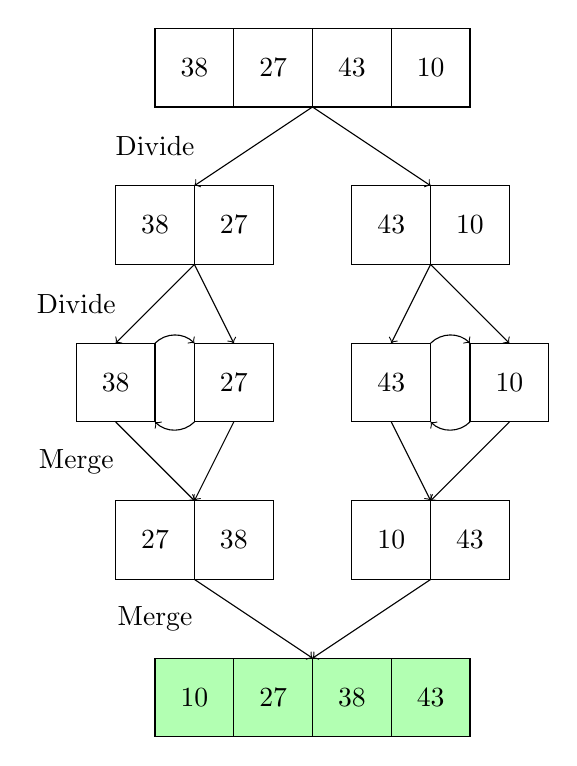
\begin{tikzpicture}
        % Initial
        \draw (0, 0) rectangle (1, 1);
        \node at (0.5, 0.5) {38};
        \draw (1, 0) rectangle (2, 1);
        \node at (1.5, 0.5) {27};
        \draw (2, 0) rectangle (3, 1);
        \node at (2.5, 0.5) {43};
        \draw (3, 0) rectangle (4, 1);
        \node at (3.5, 0.5) {10};

        % 1st Divide
        \draw (-0.5, -2) rectangle (0.5, -1);
        \node at (0, -1.5) {38};
        \draw (0.5, -2) rectangle (1.5, -1);
        \node at (1, -1.5) {27};

        \draw (2.5, -2) rectangle (3.5, -1);
        \node at (3, -1.5) {43};
        \draw (3.5, -2) rectangle (4.5, -1);
        \node at (4, -1.5) {10};

        % 2nd Divide
        \draw (-1, -4) rectangle (0, -3);
        \node at (-0.5, -3.5) {38};
        \draw (0.5, -4) rectangle (1.5, -3);
        \node at (1, -3.5) {27};

        \draw (2.5, -4) rectangle (3.5, -3);
        \node at (3, -3.5) {43};
        \draw (4, -4) rectangle (5, -3);
        \node at (4.5, -3.5) {10};

        \draw[->, bend left=45] (0, -3) to (0.5, -3);
        \draw[->, bend left=45] (0.5, -4) to (0, -4);

        \draw[->, bend left=45] (3.5, -3) to (4, -3);
        \draw[->, bend left=45] (4, -4) to (3.5, -4);

        % 1st Merge
        \draw (-0.5, -6) rectangle (0.5, -5);
        \node at (0, -5.5) {27};
        \draw (0.5, -6) rectangle (1.5, -5);
        \node at (1, -5.5) {38};

        \draw (2.5, -6) rectangle (3.5, -5);
        \node at (3, -5.5) {10};
        \draw (3.5, -6) rectangle (4.5, -5);
        \node at (4, -5.5) {43};
        
        % 2nd Merge
        \draw[fill=green!30] (0, -8) rectangle (1, -7);
        \node at (0.5, -7.5) {10};
        \draw[fill=green!30] (1, -8) rectangle (2, -7);
        \node at (1.5, -7.5) {27};
        \draw[fill=green!30] (2, -8) rectangle (3, -7);
        \node at (2.5, -7.5) {38};
        \draw[fill=green!30] (3, -8) rectangle (4, -7);
        \node at (3.5, -7.5) {43};

        % Connections
        % 1st Divide
        \draw[->] (2, 0) -- (0.5, -1);
        \draw[->] (2, 0) -- (3.5, -1);
        \node at (0, -0.5) {Divide};

        % 2nd Divide
        \draw[->] (0.5, -2) -- (-0.5, -3);
        \draw[->] (0.5, -2) -- (1, -3);

        \draw[->] (3.5, -2) -- (3, -3);
        \draw[->] (3.5, -2) -- (4.5, -3);

        \node at (-1, -2.5) {Divide};

        % 1st Merge
        \draw[->] (-0.5, -4) -- (0.5, -5);
        \draw[->] (1, -4) -- (0.5, -5);

        \draw[->] (3, -4) -- (3.5, -5);
        \draw[->] (4.5, -4) -- (3.5, -5);

        \node at (-1, -4.5) {Merge};

        % 2nd Merge
        \draw[->] (0.5, -6) -- (2, -7);
        \draw[->] (3.5, -6) -- (2, -7);

        \node at (0, -6.5) {Merge};
    \end{tikzpicture}
    \caption{Merge Sort}
    \label{fig:merge-sort}
\end{figure}

Figure \ref{fig:merge-sort} shows the Merge Sort algorithm in action.
The algorithm sorts an array of elements by dividing the array into two
halves, recursively sorting the two halves, and then merging the sorted
halves. In each step, the algorithm divides the array into smaller
subarrays until each subarray contains only one element. It then merges
the subarrays in a sorted order to produce the final sorted array.

\subsubsection{Algorithm of Merge Sort}

\begin{itemize}
    \item Divide the input array into two halves.
    
    \item Recursively sort the two halves.
    
    \item Merge the sorted halves to produce the final sorted array.
\end{itemize}

\subsubsection{Pseudo-code of Merge Sort}

\begin{lstlisting}[caption={Merge Sort Pseudo-code}]
Merge(arr, left, mid, right)
    n1 = mid - left + 1
    n2 = right - mid

    L[1..n1], R[1..n2]

    for i = 0 to n1 -  1 
        L[i] = arr[left + i]

    for j = 0 to n2 - 1
        R[j] = arr[mid + 1 + j]

    i = 0, j = 0, k = left

    while i < n1 and j < n2
        if L[i] <= R[j]
            arr[k] = L[i]
            i++
        else
            arr[k] = R[j]
            j++
        k++

    while i < n1
        arr[k] = L[i]
        i++
        k++

    while j < n2
        arr[k] = R[j]
        j++
        k++

MergeSort(arr, left, right)
    if left < right
        mid = left + (right - left) / 2

        MergeSort(arr, left, mid)
        MergeSort(arr, mid + 1, right)

        Merge(arr, left, mid, right)
\end{lstlisting}

Pseudo-code for Merge Sort is shown in the code snippet. The algorithm
takes an array of elements as input and sorts the array using the Merge
Sort technique. The algorithm divides the array into two halves, recursively
sorts the two halves, and then merges the sorted halves to produce the
final sorted array.

\subsubsection{Merge Sort in C++}

\begin{lstlisting}[language=C++, caption={Merge Sort in C++}, label={lst:merge-sort-cpp}]
#include <iostream>
#include <vector>
using namespace std;

void merge(vector<int> &arr, int left, int mid, int right) {
    int n1 = mid - left + 1;
    int n2 = right - mid;

    vector<int> L(n1), R(n2);

    for (int i = 0; i < n1; i++) {
        L[i] = arr[left + i];
    }

    for (int j = 0; j < n2; j++) {
        R[j] = arr[mid + 1 + j];
    }

    int i = 0, j = 0, k = left;

    while (i < n1 && j < n2) {
        if (L[i] <= R[j]) {
            arr[k] = L[i];
            i++;
        } else {
            arr[k] = R[j];
            j++;
        }
        k++;
    }

    while (i < n1) {
        arr[k] = L[i];
        i++;
        k++;
    }

    while (j < n2) {
        arr[k] = R[j];
        j++;
        k++;
    }
}

void mergeSort(vector<int> &arr, int left, int right) {
    if (left < right) {
        int mid = left + (right - left) / 2;

        mergeSort(arr, left, mid);
        mergeSort(arr, mid + 1, right);

        merge(arr, left, mid, right);
    }
}

void printArray(vector<int> &arr) {
    for (int i = 0; i < arr.size(); i++) {
        cout << arr[i] << " ";
    }
    cout << endl;
}

int main() {
    vector<int> arr = {38, 27, 43, 10};

    cout << "Original Array: ";
    printArray(arr);

    mergeSort(arr, 0, arr.size() - 1);

    cout << "Sorted Array: ";
    printArray(arr);

    return 0;
}
\end{lstlisting}

Code \ref{lst:merge-sort-cpp} shows the implementation of the Merge Sort
algorithm in C++. The code snippet defines a function \texttt{mergeSort}
that takes a vector of integers as input and sorts the array using the
Merge Sort technique. The algorithm divides the array into two halves,
recursively sorts the two halves, and then merges the sorted halves to
produce the final sorted array. In the example, the Merge Sort algorithm
is used to sort an array of elements, and the sorted array is printed to
the console.

\subsubsection{Applications of Merge Sort}

\begin{itemize}
    \item Merge Sort is suitable for sorting large datasets efficiently.
    
    \item It is used in external sorting when the dataset is too large to
    fit in memory.
    
    \item Merge Sort is used in inversion counting, where the number of
    inversions in an array is calculated.
    
    \item Merge Sort and its variations are used in library methods of
    programming languages. For example, its variation TimSort is used in
    Python, Java, Android, and Swift.
    
    \item It is a preferred algorithm for sorting linked lists due to its
    efficient use of memory.
    
    \item Merge Sort can be easily parallelized as subarrays can be
    independently sorted and then merged.
    
    \item The merge function of Merge Sort can be used to efficiently solve
    problems like the union and intersection of two sorted arrays.
\end{itemize}

\subsubsection{Advantages and Disadvantages of Merge Sort}

\textbf{Advantages}:

\begin{itemize}
    \item Stable sorting algorithm that maintains the relative order of
    equal elements.
    
    \item Guaranteed worst-case performance of \texttt{$O(n \log n)$},
    making it efficient for large datasets.
    
    \item Simple to implement using the divide-and-conquer approach.
    
    \item Naturally parallelizable, as subarrays can be independently
    sorted and then merged.
\end{itemize}

\textbf{Disadvantages}:

\begin{itemize}
    \item Requires additional memory for storing the merged subarrays,
    leading to a space complexity of \texttt{$O(n)$}.
    
    \item Not an in-place sorting algorithm, which can be a disadvantage
    in memory-constrained applications.
    
    \item Slower than Quick Sort in general due to additional memory
    requirements and slower cache performance.
\end{itemize}

\subsubsection{Complexity Analysis of Merge Sort}

The time complexity of Merge Sort is \texttt{$O(n \log n)$} in the
worst-case scenario, where \texttt{$n$} is the number of elements in
the array. The space complexity of Merge Sort is \texttt{$O(n)$} due
to the additional memory required for merging the subarrays.

\subsection{Quick Sort}

Quick Sort is a comparison-based sorting algorithm that uses a
divide-and-conquer strategy to sort an array of elements. It is one
of the most efficient sorting algorithms with an average-case time
complexity of \texttt{$O(n \log n)$}. Quick Sort works by selecting
a pivot element from the array, partitioning the array into two
subarrays based on the pivot, and recursively sorting the subarrays.

% Create a TikzPicture
\begin{figure}[h!]
    \centering
    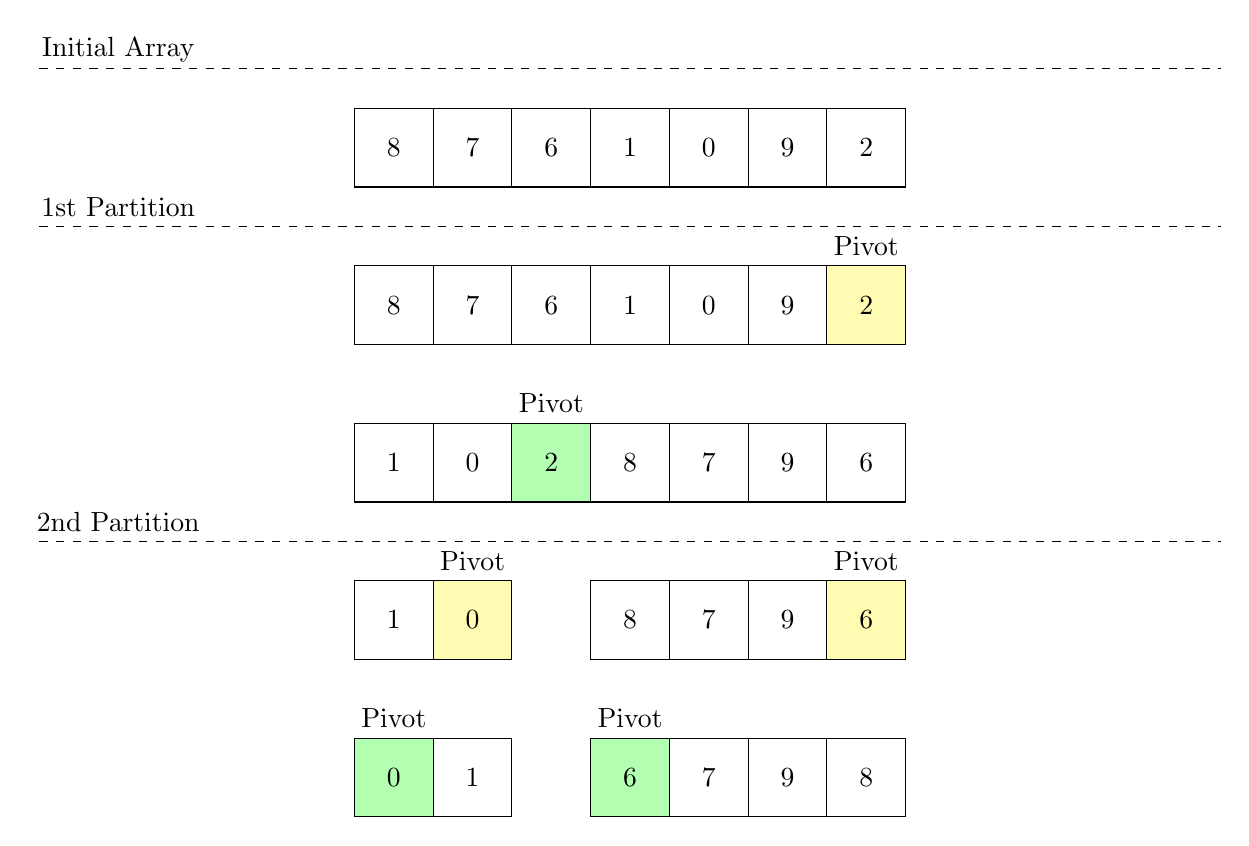
\begin{tikzpicture}
        % Initial
        \node at (-3, 1.75) {Initial Array};
        \draw[dashed] (-4, 1.5) -- (11, 1.5);
        
        \draw (0, 0) rectangle (1, 1);
        \node at (0.5, 0.5) {8};
        \draw (1, 0) rectangle (2, 1);
        \node at (1.5, 0.5) {7};
        \draw (2, 0) rectangle (3, 1);
        \node at (2.5, 0.5) {6};
        \draw (3, 0) rectangle (4, 1);
        \node at (3.5, 0.5) {1};
        \draw (4, 0) rectangle (5, 1);
        \node at (4.5, 0.5) {0};
        \draw (5, 0) rectangle (6, 1);
        \node at (5.5, 0.5) {9};
        \draw (6, 0) rectangle (7, 1);
        \node at (6.5, 0.5) {2};

        % 1st Partition
        \node at (-3, -0.25) {1st Partition};
        \draw[dashed] (-4, -0.5) -- (11, -0.5);

        \draw (0, -2) rectangle (1, -1);
        \node at (0.5, -1.5) {8};
        \draw (1, -2) rectangle (2, -1);
        \node at (1.5, -1.5) {7};
        \draw (2, -2) rectangle (3, -1);
        \node at (2.5, -1.5) {6};
        \draw (3, -2) rectangle (4, -1);
        \node at (3.5, -1.5) {1};
        \draw (4, -2) rectangle (5, -1);
        \node at (4.5, -1.5) {0};
        \draw (5, -2) rectangle (6, -1);
        \node at (5.5, -1.5) {9};
        \draw[fill=yellow!30] (6, -2) rectangle (7, -1);
        \node at (6.5, -1.5) {2};

        \node at (6.5, -0.75) {Pivot};

        % 1st Partition - FINAL
        \draw (0, -4) rectangle (1, -3);
        \node at (0.5, -3.5) {1};
        \draw (1, -4) rectangle (2, -3);
        \node at (1.5, -3.5) {0};
        \draw[fill=green!30] (2, -4) rectangle (3, -3);
        \node at (2.5, -3.5) {2};
        \draw (3, -4) rectangle (4, -3);
        \node at (3.5, -3.5) {8};
        \draw (4, -4) rectangle (5, -3);
        \node at (4.5, -3.5) {7};
        \draw (5, -4) rectangle (6, -3);
        \node at (5.5, -3.5) {9};
        \draw (6, -4) rectangle (7, -3);
        \node at (6.5, -3.5) {6};

        \node at (2.5, -2.75) {Pivot};

        % 2nd Partition
        \node at (-3, -4.25) {2nd Partition};
        \draw[dashed] (-4, -4.5) -- (11, -4.5);

        \draw (0, -6) rectangle (1, -5);
        \node at (0.5, -5.5) {1};
        \draw[fill=yellow!30] (1, -6) rectangle (2, -5);
        \node at (1.5, -5.5) {0};

        \node at (1.5, -4.75) {Pivot};

        \draw (3, -6) rectangle (4, -5);
        \node at (3.5, -5.5) {8};
        \draw (4, -6) rectangle (5, -5);
        \node at (4.5, -5.5) {7};
        \draw (5, -6) rectangle (6, -5);
        \node at (5.5, -5.5) {9};
        \draw[fill=yellow!30] (6, -6) rectangle (7, -5);
        \node at (6.5, -5.5) {6};

        \node at (6.5, -4.75) {Pivot};

        % 2nd Partition - FINAL
        \draw[fill=green!30] (0, -8) rectangle (1, -7);
        \node at (0.5, -7.5) {0};
        \draw (1, -8) rectangle (2, -7);
        \node at (1.5, -7.5) {1};

        \node at (0.5, -6.75) {Pivot};

        \draw[fill=green!30] (3, -8) rectangle (4, -7);
        \node at (3.5, -7.5) {6};
        \draw (4, -8) rectangle (5, -7);
        \node at (4.5, -7.5) {7};
        \draw (5, -8) rectangle (6, -7);
        \node at (5.5, -7.5) {9};
        \draw (6, -8) rectangle (7, -7);
        \node at (6.5, -7.5) {8};

        \node at (3.5, -6.75) {Pivot};
    \end{tikzpicture}
    % \caption{Quick Sort}
    % \label{fig:quick-sort}
\end{figure}

\begin{figure}[h!]
    \centering
    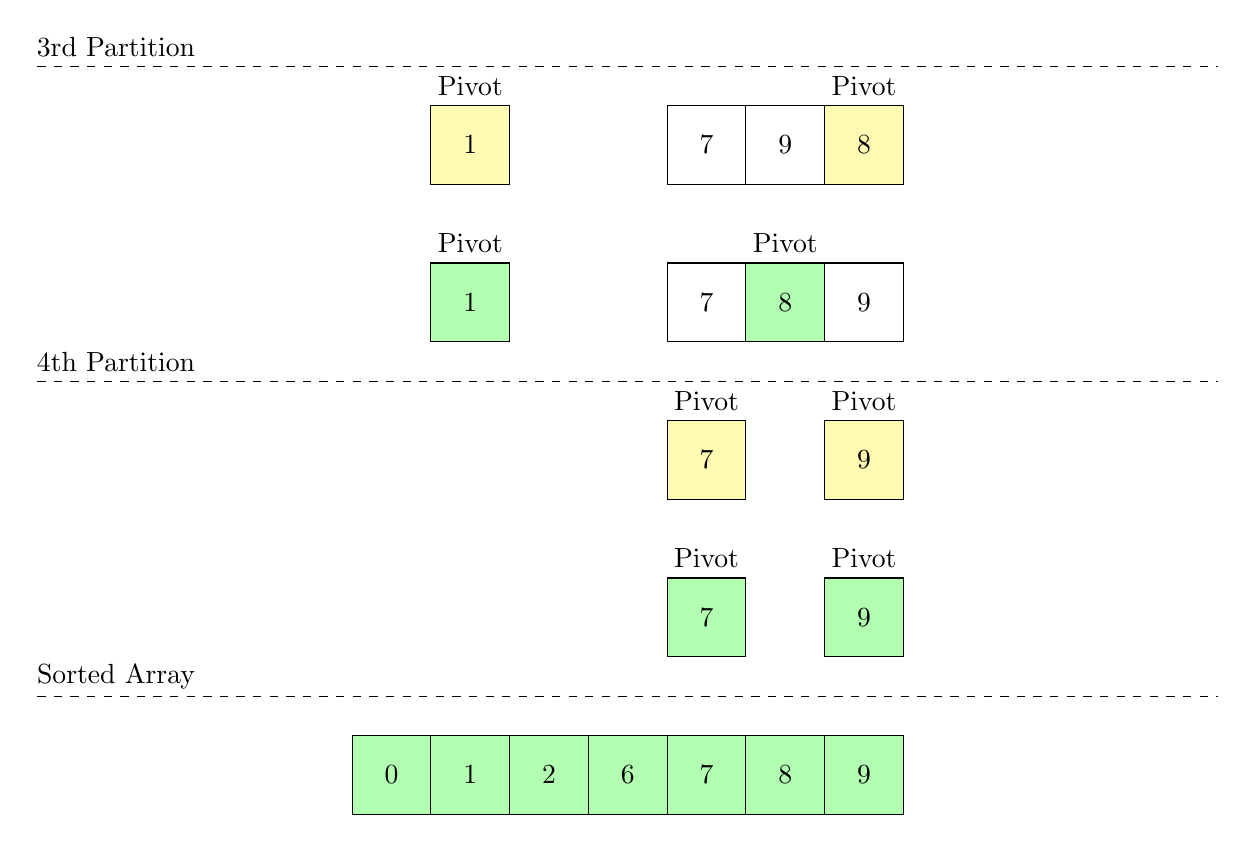
\begin{tikzpicture}
        % 3rd Partition
        \node at (-3, 1.75) {3rd Partition};
        \draw[dashed] (-4, 1.5) -- (11, 1.5);

        \draw[fill=yellow!30] (1, 0) rectangle (2, 1);
        \node at (1.5, 0.5) {1};

        \node at (1.5, 1.25) {Pivot};

        \draw (4, 0) rectangle (5, 1);
        \node at (4.5, 0.5) {7};
        \draw (5, 0) rectangle (6, 1);
        \node at (5.5, 0.5) {9};
        \draw[fill=yellow!30] (6, 0) rectangle (7, 1);
        \node at (6.5, 0.5) {8};

        \node at (6.5, 1.25) {Pivot};
        
        % 3rd Partition - FINAL
        \draw[fill=green!30] (1, -2) rectangle (2, -1);
        \node at (1.5, -1.5) {1};

        \node at (1.5, -0.75) {Pivot};

        \draw (4, -2) rectangle (5, -1);
        \node at (4.5, -1.5) {7};
        \draw[fill=green!30] (5, -2) rectangle (6, -1);
        \node at (5.5, -1.5) {8};
        \draw (6, -2) rectangle (7, -1);
        \node at (6.5, -1.5) {9};

        \node at (5.5, -0.75) {Pivot};

        % 4th Partition
        \node at (-3, -2.25) {4th Partition};
        \draw[dashed] (-4, -2.5) -- (11, -2.5);

        \draw[fill=yellow!30] (4, -4) rectangle (5, -3);
        \node at (4.5, -3.5) {7};
        
        \node at (4.5, -2.75) {Pivot};
        
        \draw[fill=yellow!30] (6, -4) rectangle (7, -3);
        \node at (6.5, -3.5) {9};

        \node at (6.5, -2.75) {Pivot};

        % 4th Partition - FINAL
        \draw[fill=green!30] (4, -6) rectangle (5, -5);
        \node at (4.5, -5.5) {7};

        \node at (4.5, -4.75) {Pivot};

        \draw[fill=green!30] (6, -6) rectangle (7, -5);
        \node at (6.5, -5.5) {9};

        \node at (6.5, -4.75) {Pivot};

        % Sorted Array
        \node at (-3, -6.25) {Sorted Array};
        \draw[dashed] (-4, -6.5) -- (11, -6.5);

        \draw[fill=green!30] (0, -8) rectangle (1, -7);
        \node at (0.5, -7.5) {0};
        \draw[fill=green!30] (1, -8) rectangle (2, -7);
        \node at (1.5, -7.5) {1};
        \draw[fill=green!30] (2, -8) rectangle (3, -7);
        \node at (2.5, -7.5) {2};
        \draw[fill=green!30] (3, -8) rectangle (4, -7);
        \node at (3.5, -7.5) {6};
        \draw[fill=green!30] (4, -8) rectangle (5, -7);
        \node at (4.5, -7.5) {7};
        \draw[fill=green!30] (5, -8) rectangle (6, -7);
        \node at (5.5, -7.5) {8};
        \draw[fill=green!30] (6, -8) rectangle (7, -7);
        \node at (6.5, -7.5) {9};
    \end{tikzpicture}
    \caption{Quick Sort}
    \label{fig:quick-sort}
\end{figure}

Figure \ref{fig:quick-sort} shows the Quick Sort algorithm in action.
The algorithm sorts an array of elements by selecting a pivot element,
partitioning the array into two subarrays based on the pivot, and
recursively sorting the subarrays. In each step, the algorithm selects
a pivot element, partitions the array into smaller subarrays, and then
repeats the process until the entire array is sorted.

\subsubsection{Algorithm of Quick Sort}

\begin{itemize}
    \item Select a pivot element from the array.
    
    \item Partition the array into two subarrays: elements less than
    the pivot and elements greater than the pivot.
    
    \item Recursively sort the two subarrays.
\end{itemize}

\subsubsection{Pseudo-code of Quick Sort}

\begin{lstlisting}[caption={Quick Sort Pseudo-code}]
Partition(arr, low, high)
    pivot = arr[high]
    i = low

    for j = low to high - 1
        if arr[j] < pivot
            swap arr[i] and arr[j]
            i++

    swap arr[i] and arr[high]
    return i

QuickSort(arr, low, high)
    if low < high
        pi = Partition(arr, low, high)

        QuickSort(arr, low, pi - 1)
        QuickSort(arr, pi + 1, high)
\end{lstlisting}

Pseudo-code for Quick Sort is shown in the code snippet. The algorithm
takes an array of elements as input and sorts the array using the Quick
Sort technique. The algorithm selects a pivot element from the array,
partitions the array into two subarrays based on the pivot, and 
recursively sorts the subarrays.

\subsubsection{Quick Sort in C++}

\begin{lstlisting}[language=C++, caption={Quick Sort in C++}, label={lst:quick-sort-cpp}]
#include <iostream>
#include <vector>
using namespace std;

int partition(vector<int> &arr, int low, int high) {
    int pivot = arr[high];
    int i = low;

    for (int j = low; j < high; j++) {
        if (arr[j] < pivot) {
            swap(arr[i], arr[j]);
            i++;
        }
    }

    swap(arr[i], arr[high]);
    return i;
}

void quickSort(vector<int> &arr, int low, int high) {
    if (low < high) {
        int pi = partition(arr, low, high);

        quickSort(arr, low, pi - 1);
        quickSort(arr, pi + 1, high);
    }
}

void printArray(vector<int> &arr) {
    for (int i = 0; i < arr.size(); i++) {
        cout << arr[i] << " ";
    }
    cout << endl;
}

int main() {
    vector<int> arr = {8, 7, 6, 1, 0, 9, 2};

    cout << "Original Array: ";
    printArray(arr);

    quickSort(arr, 0, arr.size() - 1);

    cout << "Sorted Array: ";
    printArray(arr);

    return 0;
}
\end{lstlisting}

Code \ref{lst:quick-sort-cpp} shows the implementation of the Quick Sort
algorithm in C++. The code snippet defines a function \texttt{quickSort}
that takes a vector of integers as input and sorts the array using the
Quick Sort technique. The algorithm selects a pivot element from the array,
partitions the array into two subarrays based on the pivot, and recursively
sorts the subarrays. In the example, the Quick Sort algorithm is used to
sort an array of elements, and the sorted array is printed to the console.

\subsubsection{Applications of Quick Sort}

\begin{itemize}
    \item Quick Sort is efficient for sorting large datasets with an
    average-case time complexity of \texttt{$O(n \log n)$}.
    
    \item It is used in partitioning problems like finding the $kth$
    smallest element or dividing arrays by a pivot.
    
    \item Quick Sort is integral to randomized algorithms, offering
    better performance than deterministic approaches.
    
    \item It is applied in cryptography for generating random 
    permutations and unpredictable encryption keys.
    
    \item The partitioning step of Quick Sort can be parallelized for 
    improved performance in multi-core or distributed systems.
    
    \item Quick Sort is important in theoretical computer science for 
    analyzing average-case complexity and developing new techniques.
\end{itemize}

\subsubsection{Advantages and Disadvantages of Quick Sort}

\textbf{Advantages}:

\begin{itemize}
    \item Divide-and-conquer algorithm that simplifies problem-solving.
    
    \item Efficient on large datasets with an average-case time complexity
    of \texttt{$O(n \log n)$}.
    
    \item Low overhead and memory requirements, making it suitable for
    memory-constrained applications.
    
    \item Cache-friendly algorithm that operates on the same array to
    sort without copying data to auxiliary arrays.
    
    \item Fastest general-purpose algorithm for large datasets when
    stability is not required.
    
    \item Tail-recursive, allowing tail call optimization for improved
    performance.
\end{itemize}

\textbf{Disadvantages}:

\begin{itemize}
    \item Worst-case time complexity of \texttt{$O(n^2)$} when the pivot
    is chosen poorly.
    
    \item Not suitable for small datasets due to overhead and partitioning
    costs.
    
    \item Not a stable sort, meaning that the relative order of equal
    elements may not be preserved in the sorted output.
\end{itemize}

\subsubsection{Complexity Analysis of Quick Sort}

The worst-case time complexity of Quick Sort is \texttt{$O(n^2)$}, which
occurs when the pivot element is chosen poorly. However, the average-case
time complexity of Quick Sort is \texttt{$O(n \log n)$}, making it efficient
for large datasets. The space complexity of Quick Sort is \texttt{$O(\log n)$}
due to the recursive calls and partitioning steps.

\subsection{Heap Sort}

Heap Sort is a comparison-based sorting algorithm that uses a binary heap
data structure to sort an array of elements. It is an in-place sorting
algorithm with a time complexity of \texttt{$O(n \log n)$} in the worst-case
scenario. Heap Sort works by building a max heap from the input array,
repeatedly extracting the maximum element from the heap, and then
reconstructing the heap.

% Create a TikzPicture
\begin{figure}[h!]
    \centering
    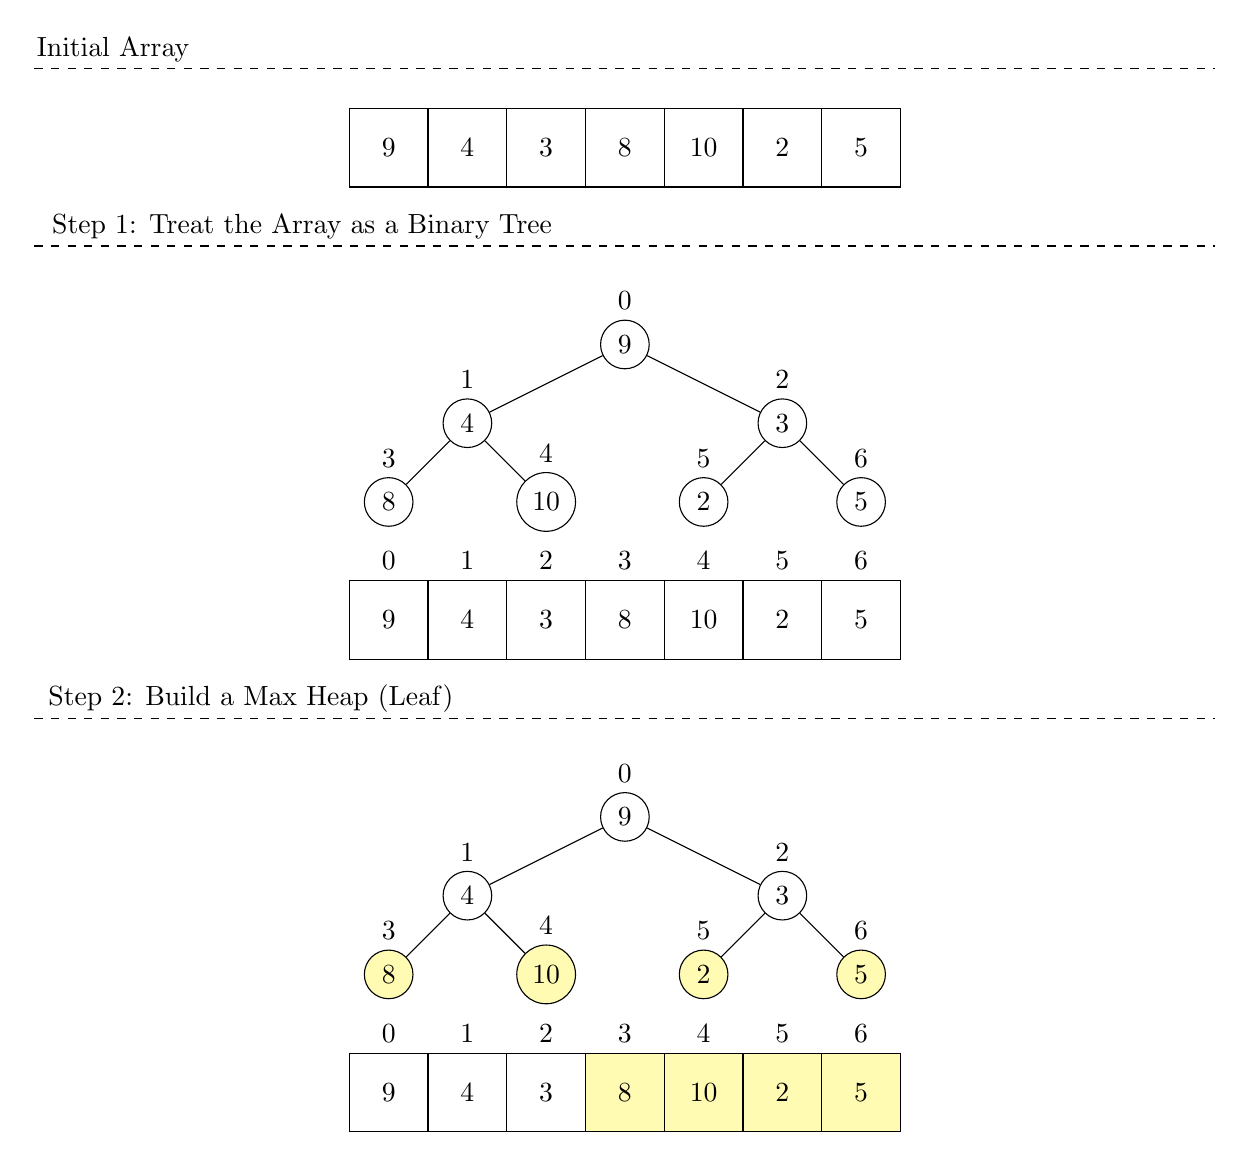
\begin{tikzpicture}
        \begin{scope}
            \node at (-3, 1.75) {Initial Array};
            \draw[dashed] (-4, 1.5) -- (11, 1.5);

            \draw (0, 0) rectangle (1, 1);
            \node at (0.5, 0.5) {9};
            \draw (1, 0) rectangle (2, 1);
            \node at (1.5, 0.5) {4};
            \draw (2, 0) rectangle (3, 1);
            \node at (2.5, 0.5) {3};
            \draw (3, 0) rectangle (4, 1);
            \node at (3.5, 0.5) {8};
            \draw (4, 0) rectangle (5, 1);
            \node at (4.5, 0.5) {10};
            \draw (5, 0) rectangle (6, 1);
            \node at (5.5, 0.5) {2};
            \draw (6, 0) rectangle (7, 1);
            \node at (6.5, 0.5) {5};
        \end{scope}

        \begin{scope}
            % \draw (1.5, -1.5) circle (0.5);
            % \node at (1.5, -1.5) {30};
            
            % Step 1: Treat Array as a Binary Tree
            \node at (-0.6, -0.5) {Step 1: Treat the Array as a Binary Tree};
            \draw[dashed] (-4, -0.75) -- (11, -0.75);

            % Create Binary Tree
            \node[draw, circle, label=above:0] (a) at (3.5, -2) {9};
            \node[draw, circle, label=above:1] (b) at (1.5, -3) {4};
            \node[draw, circle, label=above:2] (c) at (5.5, -3) {3};
            \node[draw, circle, label=above:3] (d) at (0.5, -4) {8};
            \node[draw, circle, label=above:4] (e) at (2.5, -4) {10};
            \node[draw, circle, label=above:5] (f) at (4.5, -4) {2};
            \node[draw, circle, label=above:6] (g) at (6.5, -4) {5};

            % Connect Nodes
            \draw (a) -- (b);
            \draw (a) -- (c);
            \draw (b) -- (d);
            \draw (b) -- (e);
            \draw (c) -- (f);
            \draw (c) -- (g);

            % Array
            \draw (0, -6) rectangle (1, -5);
            \node at (0.5, -5.5) {9};
            \node at (0.5, -4.75) {0};
            \draw (1, -6) rectangle (2, -5);
            \node at (1.5, -5.5) {4};
            \node at (1.5, -4.75) {1};
            \draw (2, -6) rectangle (3, -5);
            \node at (2.5, -5.5) {3};
            \node at (2.5, -4.75) {2};
            \draw (3, -6) rectangle (4, -5);
            \node at (3.5, -5.5) {8};
            \node at (3.5, -4.75) {3};
            \draw (4, -6) rectangle (5, -5);
            \node at (4.5, -5.5) {10};
            \node at (4.5, -4.75) {4};
            \draw (5, -6) rectangle (6, -5);
            \node at (5.5, -5.5) {2};
            \node at (5.5, -4.75) {5};
            \draw (6, -6) rectangle (7, -5);
            \node at (6.5, -5.5) {5};
            \node at (6.5, -4.75) {6};
        \end{scope}

        \begin{scope}
            % Step 2: Build a Max Heap
            \node at (-1.25, -6.5) {Step 2: Build a Max Heap (Leaf)};
            \draw[dashed] (-4, -6.75) -- (11, -6.75);

            % Create Binary Tree
            \node[draw, circle, label=above:0] (a) at (3.5, -8) {9};
            \node[draw, circle, label=above:1] (b) at (1.5, -9) {4};
            \node[draw, circle, label=above:2] (c) at (5.5, -9) {3};
            \node[draw, circle, label=above:3, fill=yellow!30] (d) at (0.5, -10) {8};
            \node[draw, circle, label=above:4, fill=yellow!30] (e) at (2.5, -10) {10};
            \node[draw, circle, label=above:5, fill=yellow!30] (f) at (4.5, -10) {2};
            \node[draw, circle, label=above:6, fill=yellow!30] (g) at (6.5, -10) {5};

            % Connect Nodes
            \draw (a) -- (b);
            \draw (a) -- (c);
            \draw (b) -- (d);
            \draw (b) -- (e);
            \draw (c) -- (f);
            \draw (c) -- (g);

            % Array
            \draw (0, -12) rectangle (1, -11);
            \node at (0.5, -11.5) {9};
            \node at (0.5, -10.75) {0};
            \draw (1, -12) rectangle (2, -11);
            \node at (1.5, -11.5) {4};
            \node at (1.5, -10.75) {1};
            \draw (2, -12) rectangle (3, -11);
            \node at (2.5, -11.5) {3};
            \node at (2.5, -10.75) {2};
            \draw[fill=yellow!30] (3, -12) rectangle (4, -11);
            \node at (3.5, -11.5) {8};
            \node at (3.5, -10.75) {3};
            \draw[fill=yellow!30] (4, -12) rectangle (5, -11);
            \node at (4.5, -11.5) {10};
            \node at (4.5, -10.75) {4};
            \draw[fill=yellow!30] (5, -12) rectangle (6, -11);
            \node at (5.5, -11.5) {2};
            \node at (5.5, -10.75) {5};
            \draw[fill=yellow!30] (6, -12) rectangle (7, -11);
            \node at (6.5, -11.5) {5};
            \node at (6.5, -10.75) {6};
        \end{scope}
    \end{tikzpicture}
    % \caption{Heap Sort}
    % \label{fig:heap-sort}
\end{figure}

\begin{figure}[h!]
    \centering
    \begin{tikzpicture}
        \begin{scope}
            % Step 2: Build a Max Heap (1st Swap)
            \node at (-0.1, 1.25) {Step 2: Build a Max Heap (Heapify 2nd Level)};
            \draw[dashed] (-4, 1) -- (11, 1);

            \begin{scope}
                \node[text width=3.5cm] (search) [box rounded] at (-2, -1) {
                    % Swap 4 and 10 since 4 is the parent and 10 is the
                    % child. 10 is greater than 4, so swap them.
                    Swap 4 and 10
                    \begin{itemize}
                        \item 10 is the largest element.
                        \item 10 is greater than 4 and 8.
                    \end{itemize}
                };
                

                % Create Binary Tree
                \node[draw, circle, label=above:0] (a) at (3.5, 0) {9};
                \node[draw, circle, label=above:1, fill=yellow!30] (b) at (1.5, -1) {4};
                \node[draw, circle, label=above:2] (c) at (5.5, -1) {3};
                \node[draw, circle, label=above:3, fill=yellow!30] (d) at (0.5, -2) {8};
                \node[draw, circle, label=above:4, fill=yellow!30] (e) at (2.5, -2) {10};
                \node[draw, circle, label=above:5] (f) at (4.5, -2) {2};
                \node[draw, circle, label=above:6] (g) at (6.5, -2) {5};

                % Connect Nodes
                \draw (a) -- (b);
                \draw (a) -- (c);
                \draw (b) -- (d);
                \draw (b) -- (e);
                \draw (c) -- (f);
                \draw (c) -- (g);

                % Curved Bidirectional Arrow from (b) to (e)
                \draw[->, >=stealth] (b) to[bend right=45] (e);
                \draw[->, >=stealth] (e) to[bend left=45] (b);

                % Array
                \draw (0, -4) rectangle (1, -3);
                \node at (0.5, -3.5) {9};
                \node at (0.5, -2.75) {0};
                \draw[fill=yellow!30] (1, -4) rectangle (2, -3);
                \node at (1.5, -3.5) {4};
                \node at (1.5, -2.75) {1};
                \draw (2, -4) rectangle (3, -3);
                \node at (2.5, -3.5) {3};
                \node at (2.5, -2.75) {2};
                \draw[fill=yellow!30] (3, -4) rectangle (4, -3);
                \node at (3.5, -3.5) {8};
                \node at (3.5, -2.75) {3};
                \draw[fill=yellow!30] (4, -4) rectangle (5, -3);
                \node at (4.5, -3.5) {10};
                \node at (4.5, -2.75) {4};
                \draw (5, -4) rectangle (6, -3);
                \node at (5.5, -3.5) {2};
                \node at (5.5, -2.75) {5};
                \draw (6, -4) rectangle (7, -3);
                \node at (6.5, -3.5) {5};
                \node at (6.5, -2.75) {6};

                % Bidirectional Arrow from 4 to 10
                \draw[->, >=stealth] (1.5, -4) -- (1.5, -4.25) -- (4.5, -4.25) -- (4.5, -4);
                \draw[->, >=stealth] (4.5, -4) -- (4.5, -4.25) -- (1.5, -4.25) -- (1.5, -4);
                \node at (3, -4.5) {Swap};
            \end{scope}

            \begin{scope}
                \node[text width=3.5cm] (search) [box rounded] at (-2, -7) {
                    % Swap 3 and 5 since 3 is the parent and 5 is the
                    % child. 5 is greater than 3, so swap them.
                    Swap 3 and 5
                    \begin{itemize}
                        \item 5 is the largest element.
                        \item 5 is greater than 3 and 2.
                    \end{itemize}
                };

                % Create Binary Tree
                \node[draw, circle, label=above:0] (a) at (3.5, -6) {9};
                \node[draw, circle, label=above:1] (b) at (1.5, -7) {4};
                \node[draw, circle, label=above:2, fill=yellow!30] (c) at (5.5, -7) {3};
                \node[draw, circle, label=above:3] (d) at (0.5, -8) {8};
                \node[draw, circle, label=above:4] (e) at (2.5, -8) {10};
                \node[draw, circle, label=above:5, fill=yellow!30] (f) at (4.5, -8) {2};
                \node[draw, circle, label=above:6, fill=yellow!30] (g) at (6.5, -8) {5};

                % Connect Nodes
                \draw (a) -- (b);
                \draw (a) -- (c);
                \draw (b) -- (d);
                \draw (b) -- (e);
                \draw (c) -- (f);
                \draw (c) -- (g);

                % Curved Bidirectional Arrow from (c) to (g)
                \draw[->, >=stealth] (c) to[bend right=45] (g);
                \draw[->, >=stealth] (g) to[bend left=45] (c);

                % Array
                \draw (0, -10) rectangle (1, -9);
                \node at (0.5, -9.5) {9};
                \node at (0.5, -8.75) {0};
                \draw (1, -10) rectangle (2, -9);
                \node at (1.5, -9.5) {4};
                \node at (1.5, -8.75) {1};
                \draw[fill=yellow!30] (2, -10) rectangle (3, -9);
                \node at (2.5, -9.5) {3};
                \node at (2.5, -8.75) {2};
                \draw (3, -10) rectangle (4, -9);
                \node at (3.5, -9.5) {8};
                \node at (3.5, -8.75) {3};
                \draw (4, -10) rectangle (5, -9);
                \node at (4.5, -9.5) {10};
                \node at (4.5, -8.75) {4};
                \draw[fill=yellow!30] (5, -10) rectangle (6, -9);
                \node at (5.5, -9.5) {2};
                \node at (5.5, -8.75) {5};
                \draw[fill=yellow!30] (6, -10) rectangle (7, -9);
                \node at (6.5, -9.5) {5};
                \node at (6.5, -8.75) {6};

                % Bidirectional Arrow from 3 to 5
                \draw[->, >=stealth] (2.5, -10) -- (2.5, -10.25) -- (6.5, -10.25) -- (6.5, -10);
                \draw[->, >=stealth] (6.5, -10) -- (6.5, -10.25) -- (2.5, -10.25) -- (2.5, -10);
                \node at (4.5, -10.5) {Swap};
            \end{scope}
        \end{scope}

        \begin{scope}
            % Step 2: Build a Max Heap (1st Level)
            \node at (-0.1, -10.75) {Step 2: Build a Max Heap (Heapify 1st Level)};
            \draw[dashed] (-4, -11) -- (11, -11);
            
            \node[text width=3.5cm] (search) [box rounded] at (-2, -13) {
                % Swap 9 and 10 since 9 is the parent and 10 is the
                % child. 10 is greater than 9, so swap them.
                Swap 9 and 10
                \begin{itemize}
                    \item 10 is the largest element.
                    \item 10 is greater than 9 and 8.
                \end{itemize}
            };

            % Create Binary Tree
            \node[draw, circle, label=above:0, fill=yellow!30] (a) at (3.5, -12) {9};
            \node[draw, circle, label=above:1, fill=yellow!30] (b) at (1.5, -13) {10};
            \node[draw, circle, label=above:2, fill=yellow!30] (c) at (5.5, -13) {5};
            \node[draw, circle, label=above:3] (d) at (0.5, -14) {8};
            \node[draw, circle, label=above:4] (e) at (2.5, -14) {4};
            \node[draw, circle, label=above:5] (f) at (4.5, -14) {2};
            \node[draw, circle, label=above:6] (g) at (6.5, -14) {3};

            % Connect Nodes
            \draw (a) -- (b);
            \draw (a) -- (c);
            \draw (b) -- (d);
            \draw (b) -- (e);
            \draw (c) -- (f);
            \draw (c) -- (g);

            % Curved Bidirectional Arrow from (a) to (b)
            \draw[->, >=stealth] (a) to[bend right=45] (b);
            \draw[->, >=stealth] (b) to[bend left=45] (a);

            % Array
            \draw[fill=yellow!30] (0, -16) rectangle (1, -15);
            \node at (0.5, -15.5) {9};
            \node at (0.5, -14.75) {0};
            \draw[fill=yellow!30] (1, -16) rectangle (2, -15);
            \node at (1.5, -15.5) {10};
            \node at (1.5, -14.75) {1};
            \draw[fill=yellow!30] (2, -16) rectangle (3, -15);
            \node at (2.5, -15.5) {5};
            \node at (2.5, -14.75) {2};
            \draw (3, -16) rectangle (4, -15);
            \node at (3.5, -15.5) {8};
            \node at (3.5, -14.75) {3};
            \draw (4, -16) rectangle (5, -15);
            \node at (4.5, -15.5) {4};
            \node at (4.5, -14.75) {4};
            \draw (5, -16) rectangle (6, -15);
            \node at (5.5, -15.5) {2};
            \node at (5.5, -14.75) {5};
            \draw (6, -16) rectangle (7, -15);
            \node at (6.5, -15.5) {3};
            \node at (6.5, -14.75) {6};

            % Bidirectional Arrow from 9 to 10
            \draw[->, >=stealth] (0.5, -16) -- (0.5, -16.25) -- (1.5, -16.25) -- (1.5, -16);
            \draw[->, >=stealth] (1.5, -16) -- (1.5, -16.25) -- (0.5, -16.25) -- (0.5, -16);
            \node at (1, -16.5) {Swap};
        \end{scope}

        \begin{scope}
            % Step 2: Build a Max Heap (Max Heap)
            \node at (-0.75, -17) {Step 2: Build a Max Heap (Max Heap)};
            \draw[dashed] (-4, -17.25) -- (11, -17.25);

            % Create Binary Tree
            \node[draw, circle, label=above:0] (a) at (3.5, -18.25) {10};
            \node[draw, circle, label=above:1] (b) at (1.5, -19.25) {9};
            \node[draw, circle, label=above:2] (c) at (5.5, -19.25) {5};
            \node[draw, circle, label=above:3] (d) at (0.5, -20.25) {8};
            \node[draw, circle, label=above:4] (e) at (2.5, -20.25) {4};
            \node[draw, circle, label=above:5] (f) at (4.5, -20.25) {2};
            \node[draw, circle, label=above:6] (g) at (6.5, -20.25) {3};

            % Connect Nodes
            \draw (a) -- (b);
            \draw (a) -- (c);
            \draw (b) -- (d);
            \draw (b) -- (e);
            \draw (c) -- (f);
            \draw (c) -- (g);

            % Array
            \draw (0, -22.25) rectangle (1, -21.25);
            \node at (0.5, -21.75) {10};
            \node at (0.5, -21) {0};
            \draw (1, -22.25) rectangle (2, -21.25);
            \node at (1.5, -21.75) {9};
            \node at (1.5, -21) {1};
            \draw (2, -22.25) rectangle (3, -21.25);
            \node at (2.5, -21.75) {5};
            \node at (2.5, -21) {2};
            \draw (3, -22.25) rectangle (4, -21.25);
            \node at (3.5, -21.75) {8};
            \node at (3.5, -21) {3};
            \draw (4, -22.25) rectangle (5, -21.25);
            \node at (4.5, -21.75) {4};
            \node at (4.5, -21) {4};
            \draw (5, -22.25) rectangle (6, -21.25);
            \node at (5.5, -21.75) {2};
            \node at (5.5, -21) {5};
            \draw (6, -22.25) rectangle (7, -21.25);
            \node at (6.5, -21.75) {3};
            \node at (6.5, -21) {6};
        \end{scope}
    \end{tikzpicture}
    % \caption{Heap Sort}
    % \label{fig:heap-sort}
\end{figure}

\begin{figure}[h!]
    \centering
    \begin{tikzpicture}
        % Step 3: Sort by Placing Largest Number at the End
        \node at (0.4, 1.25) {Step 3: Sort by Placing Largest Number at the End};
        \draw[dashed] (-4, 1) -- (11, 1);

        \begin{scope}
            \node[text width=3.5cm] (search) [box rounded] at (-2, -1) {
                % Swap 10 and 3 since 10 is the largest unsorted
                % element.
                Swap 10 and 3
                \begin{itemize}
                    \item 10 is the largest element among the
                    unsorted elements.
                \end{itemize}
            };

            % Create Binary Tree
            \node[draw, circle, label=above:0, fill=yellow!30] (a) at (3.5, 0) {10};
            \node[draw, circle, label=above:1] (b) at (1.5, -1) {9};
            \node[draw, circle, label=above:2] (c) at (5.5, -1) {5};
            \node[draw, circle, label=above:3] (d) at (0.5, -2) {8};
            \node[draw, circle, label=above:4] (e) at (2.5, -2) {4};
            \node[draw, circle, label=above:5] (f) at (4.5, -2) {2};
            \node[draw, circle, label=above:6, fill=yellow!30] (g) at (6.5, -2) {3};

            % Connect Nodes
            \draw (a) -- (b);
            \draw (a) -- (c);
            \draw (b) -- (d);
            \draw (b) -- (e);
            \draw (c) -- (f);
            \draw (c) -- (g);

            % Curved Bidirectional Arrow from (a) to (g)
            \draw[->, >=stealth] (a) to[bend left=45] (g);
            \draw[->, >=stealth] (g) to[bend right=45] (a);
        \end{scope}

        \begin{scope}
            % Swap 3 and 9 since 3 is the parent and 9 is the
            % largest child. 9 is greater than 3, so swap them.
            \node[text width=3.5cm] (search) [box rounded] at (-2, -4) {
                Heapify the Array
                \begin{enumerate}
                    \item Swap 3 and 9
                    \item Then, swap 3 and 8
                \end{enumerate}
            };

            % Create Binary Tree
            \node[draw, circle, label=above:0, fill=yellow!30] (a) at (3.5, -4) {3};
            \node[draw, circle, label=above:1, fill=yellow!30] (b) at (1.5, -5) {9};
            \node[draw, circle, label=above:2] (c) at (5.5, -5) {5};
            \node[draw, circle, label=above:3, fill=yellow!30] (d) at (0.5, -6) {8};
            \node[draw, circle, label=above:4] (e) at (2.5, -6) {4};
            \node[draw, circle, label=above:5] (f) at (4.5, -6) {2};
            \node[draw, circle, label=above:6, fill=green!30, dashed] (g) at (6.5, -6) {10};

            % Connect Nodes
            \draw (a) -- (b);
            \draw (a) -- (c);
            \draw (b) -- (d);
            \draw (b) -- (e);
            \draw (c) -- (f);
            \draw[dashed] (c) -- (g);

            % Curved Bidirectional Arrow from (a) to (b)
            \draw[->, >=stealth] (a) to[bend left=45] (b);
            \draw[->, >=stealth] (b) to[bend right=45] (a);
            
            % Curved Bidirectional Arrow from (b) to (d)
            \draw[->, >=stealth] (b) to[bend left=45] (d);
            \draw[->, >=stealth] (d) to[bend right=45] (b);
        \end{scope}

        \begin{scope}
            % Swap 9 and 2 since 9 is the largest unsorted
            % element.
            \node[text width=3.5cm] (search) [box rounded] at (-2, -9) {
                Swap 9 and 2
                \begin{enumerate}
                    \item Swap 9 and 2 since 9 is the largest unsorted 
                    element.
                \end{enumerate}
            };

            % Create Binary Tree
            \node[draw, circle, label=above:0, fill=yellow!30] (a) at (3.5, -8) {9};
            \node[draw, circle, label=above:1] (b) at (1.5, -9) {8};
            \node[draw, circle, label=above:2] (c) at (5.5, -9) {5};
            \node[draw, circle, label=above:3] (d) at (0.5, -10) {3};
            \node[draw, circle, label=above:4] (e) at (2.5, -10) {4};
            \node[draw, circle, label=above:5, fill=yellow!30] (f) at (4.5, -10) {2};
            \node[draw, circle, label=above:6, fill=green!30, dashed] (g) at (6.5, -10) {10};

            % Connect Nodes
            \draw (a) -- (b);
            \draw (a) -- (c);
            \draw (b) -- (d);
            \draw (b) -- (e);
            \draw[dashed] (c) -- (f);
            \draw[dashed] (c) -- (g);

            % Curved Bidirectional Arrow from (a) to (f)
            \draw[->, >=stealth] (a) to[bend right=45] (f);
            \draw[->, >=stealth] (f) to[bend left=45] (a);
        \end{scope}

        \begin{scope}
            \node[text width=3.5cm] (search) [box rounded] at (-2, -13) {
                Heapify the Array
                \begin{enumerate}
                    \item Swap 2 and 8
                    \item Then, swap 2 and 4
                \end{enumerate}
            };

            % Create Binary Tree
            \node[draw, circle, label=above:0, fill=yellow!30] (a) at (3.5, -12) {2};
            \node[draw, circle, label=above:1, fill=yellow!30] (b) at (1.5, -13) {8};
            \node[draw, circle, label=above:2] (c) at (5.5, -13) {5};
            \node[draw, circle, label=above:3] (d) at (0.5, -14) {3};
            \node[draw, circle, label=above:4, fill=yellow!30] (e) at (2.5, -14) {4};
            \node[draw, circle, label=above:5, fill=green!30, dashed] (f) at (4.5, -14) {9};
            \node[draw, circle, label=above:6, fill=green!30, dashed] (g) at (6.5, -14) {10};

            % Connect Nodes
            \draw (a) -- (b);
            \draw (a) -- (c);
            \draw (b) -- (d);
            \draw (b) -- (e);
            \draw[dashed] (c) -- (f);
            \draw[dashed] (c) -- (g);

            % Curved Bidirectional Arrow from (a) to (b)
            \draw[->, >=stealth] (a) to[bend right=45] (b);
            \draw[->, >=stealth] (b) to[bend left=45] (a);
            
            % Curved Bidirectional Arrow from (b) to (e)
            \draw[->, >=stealth] (b) to[bend right=45] (e);
            \draw[->, >=stealth] (e) to[bend left=45] (b);
        \end{scope}

        % Repeat this process until the entire array is sorted
        \node[text width=15cm] (search) [box rounded] at (3.5, -15) {
            Repeat this process until the entire array is sorted
            
            % Swap 8 and 2, Heapify, Swap 5 and 3, Heapify, Swap 4 and 2,
            % Heapify, No Swap, Heapify, No Swap, Heapify

            \textit{Swap 8 and 2, Heapify, Swap 5 and 3, Heapify, Swap 4 and 2,}
        };

        \begin{scope}
            % Sorted Array
            \node at (-2.9, -16.25) {Sorted Array};
            \draw[dashed] (-4, -16.5) -- (11, -16.5);

            \node[text width=3.5cm] (search) [box rounded] at (-2, -17.5) {
                Sorted Array:
                
                2, 3, 4, 5, 8, 9, 10
            };

            % Create Binary Tree
            \node[draw, circle, label=above:0, fill=green!30] (a) at (3.5, -17.5) {2};
            \node[draw, circle, label=above:1, fill=green!30] (b) at (1.5, -18.5) {3};
            \node[draw, circle, label=above:2, fill=green!30] (c) at (5.5, -18.5) {4};
            \node[draw, circle, label=above:3, fill=green!30] (d) at (0.5, -19.5) {5};
            \node[draw, circle, label=above:4, fill=green!30] (e) at (2.5, -19.5) {8};
            \node[draw, circle, label=above:5, fill=green!30] (f) at (4.5, -19.5) {9};
            \node[draw, circle, label=above:6, fill=green!30] (g) at (6.5, -19.5) {10};

            % Connect Nodes
            \draw (a) -- (b);
            \draw (a) -- (c);
            \draw (b) -- (d);
            \draw (b) -- (e);
            \draw (c) -- (f);
            \draw (c) -- (g);

            % Array
            \draw[fill=green!30] (0, -21.5) rectangle (1, -20.5);
            \node at (0.5, -21) {2};
            \node at (0.5, -20.25) {0};
            \draw[fill=green!30] (1, -21.5) rectangle (2, -20.5);
            \node at (1.5, -21) {3};
            \node at (1.5, -20.25) {1};
            \draw[fill=green!30] (2, -21.5) rectangle (3, -20.5);
            \node at (2.5, -21) {4};
            \node at (2.5, -20.25) {2};
            \draw[fill=green!30] (3, -21.5) rectangle (4, -20.5);
            \node at (3.5, -21) {5};
            \node at (3.5, -20.25) {3};
            \draw[fill=green!30] (4, -21.5) rectangle (5, -20.5);
            \node at (4.5, -21) {8};
            \node at (4.5, -20.25) {4};
            \draw[fill=green!30] (5, -21.5) rectangle (6, -20.5);
            \node at (5.5, -21) {9};
            \node at (5.5, -20.25) {5};
            \draw[fill=green!30] (6, -21.5) rectangle (7, -20.5);
            \node at (6.5, -21) {10};
            \node at (6.5, -20.25) {6};
        \end{scope}
    \end{tikzpicture}
    \caption{Heap Sort}
    \label{fig:heap-sort}
\end{figure}

\pagebreak

Figure \ref{fig:heap-sort} shows the Heap Sort algorithm in action. The
algorithm sorts an array of elements by building a max heap from the input
array, repeatedly extracting the maximum element from the heap, and then
reconstructing the heap. In each step, the algorithm maintains the heap
property by ensuring that the parent node is greater than its children.

\subsubsection{Algorithm of Heap Sort}

\begin{itemize}
    \item Build a max heap from the input array.
    
    \item Repeatedly extract the maximum element from the heap.
    
    \item Reconstruct the heap to maintain the heap property.
\end{itemize}

\subsubsection{Pseudo-code of Heap Sort}

\begin{lstlisting}[caption={Heap Sort Pseudo-code}]
Heapify(arr, n, i)
    largest = i
    left = 2 * i + 1
    right = 2 * i + 2

    if left < n and arr[left] > arr[largest]
        largest = left

    if right < n and arr[right] > arr[largest]
        largest = right

    if largest != i
        swap arr[i] and arr[largest]
        Heapify(arr, n, largest)

HeapSort(arr)
    n = arr.size()

    for i = n / 2 - 1 down to 0
        Heapify(arr, n, i)

    for i = n - 1 down to 1
        swap arr[0] and arr[i]
        Heapify(arr, i, 0)
\end{lstlisting}

Pseudo-code for Heap Sort is shown in the code snippet. The algorithm
takes an array of elements as input and sorts the array using the Heap
Sort technique. The algorithm builds a max heap from the input array,
repeatedly extracts the maximum element from the heap, and then
reconstructs the heap to maintain the heap property.

\subsubsection{Heap Sort in C++}

\begin{lstlisting}[language=C++, caption={Heap Sort in C++}, label={lst:heap-sort-cpp}]
#include <iostream>
#include <vector>
using namespace std;

void heapify(vector<int> &arr, int n, int i) {
    int largest = i;
    int left = 2 * i + 1;
    int right = 2 * i + 2;

    if (left < n && arr[left] > arr[largest]) {
        largest = left;
    }

    if (right < n && arr[right] > arr[largest]) {
        largest = right;
    }

    if (largest != i) {
        swap(arr[i], arr[largest]);
        heapify(arr, n, largest);
    }
}

void heapSort(vector<int> &arr) {
    int n = arr.size();

    for (int i = n / 2 - 1; i >= 0; i--) {
        heapify(arr, n, i);
    }

    for (int i = n - 1; i >= 1; i--) {
        swap(arr[0], arr[i]);
        heapify(arr, i, 0);
    }
}

void printArray(vector<int> &arr) {
    for (int i = 0; i < arr.size(); i++) {
        cout << arr[i] << " ";
    }
    cout << endl;
}

int main() {
    vector<int> arr = {9, 4, 3, 8, 10, 2, 5};

    cout << "Original Array: ";
    printArray(arr);

    heapSort(arr);

    cout << "Sorted Array: ";
    printArray(arr);

    return 0;
}
\end{lstlisting}

Code \ref{lst:heap-sort-cpp} shows the implementation of the Heap Sort
algorithm in C++. The code snippet defines a function \texttt{heapSort}
that takes a vector of integers as input and sorts the array using the
Heap Sort technique. The algorithm builds a max heap from the input
array, repeatedly extracts the maximum element from the heap, and then
reconstructs the heap. In the example, the Heap Sort algorithm is used
to sort an array of elements, and the sorted array is printed to the
console.

\subsubsection{Advantages and Disadvantages of Heap Sort}

\textbf{Advantages}:

\begin{itemize}
    \item Efficient time complexity of \texttt{$O(n \log n)$} in all cases,
    making it suitable for sorting large datasets.
    
    \item Minimal memory usage, as it requires no additional memory space
    apart from the initial list of items to be sorted.
    
    \item Simplicity in understanding compared to other equally efficient
    sorting algorithms due to the absence of advanced concepts like recursion.
\end{itemize}

\textbf{Disadvantages}:

\begin{itemize}
    \item Costly in terms of higher constants compared to other sorting
    algorithms like Merge Sort.
    
    \item Unstable sorting algorithm that might rearrange the relative order
    of equal elements.
    
    \item Inefficient due to high constants in the time complexity, making
    it slower than other sorting algorithms like Merge Sort.
\end{itemize}

\subsubsection{Complexity Analysis of Heap Sort}

The time complexity of Heap Sort is \texttt{$O(n \log n)$} in all cases,
making it efficient for sorting large datasets. The space complexity of
Heap Sort is \texttt{$O(1)$} as it is an in-place sorting algorithm that
requires no additional memory apart from the initial array.

\section{Types of Non-comparison-based Sorting Algorithms}

There are several types of non-comparison-based sorting algorithms that
sort elements based on specific properties of the input data. These
algorithms are designed to exploit certain characteristics of the data
to achieve efficient sorting without comparing elements directly. Some
common types of non-comparison-based sorting algorithms include:

\subsection{Counting Sort}

Counting Sort is a non-comparison-based sorting algorithm. It is 
particularly efficient when the range of input values is small compared 
to the number of elements to be sorted. The basic idea behind Counting 
Sort is to count the frequency of each distinct element in the input 
array and use that information to place the elements in their correct 
sorted positions.

% TikZ code for Counting Sort
\begin{figure*}[h!]
    \centering
    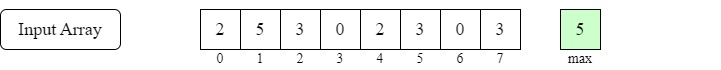
\includegraphics[width=1.0\textwidth]{./assets/images/cs2.jpg}
\end{figure*}
\begin{figure*}[h!]
    \centering
    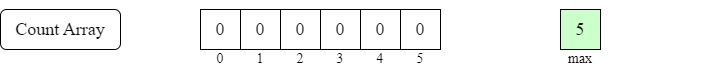
\includegraphics[width=1.0\textwidth]{./assets/images/cs3.jpg}
\end{figure*}
\begin{figure*}[h!]
    \centering
    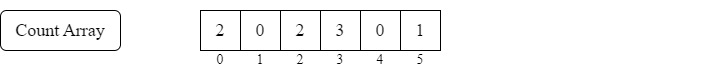
\includegraphics[width=1.0\textwidth]{./assets/images/cs4.jpg}
\end{figure*}
\begin{figure*}[h!]
    \centering
    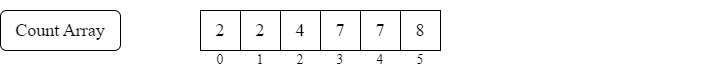
\includegraphics[width=1.0\textwidth]{./assets/images/cs5.jpg}
\end{figure*}
\begin{figure*}[h!]
    \centering
    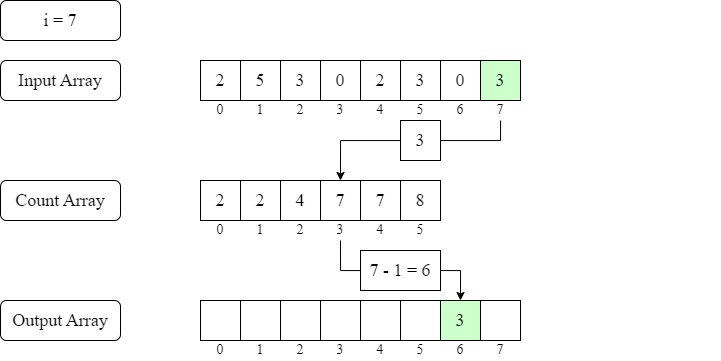
\includegraphics[width=1.0\textwidth]{./assets/images/cs6.jpg}
\end{figure*}
\begin{figure*}[h!]
    \centering
    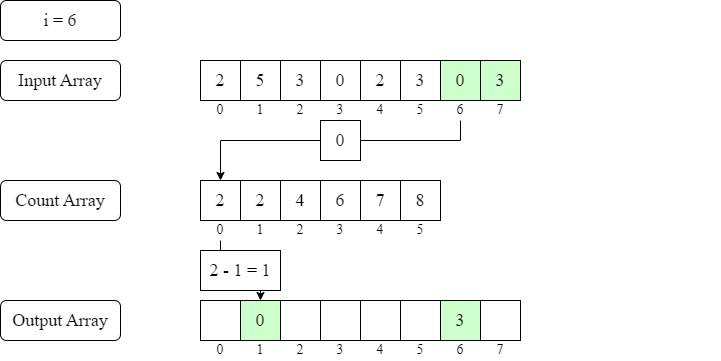
\includegraphics[width=1.0\textwidth]{./assets/images/cs7.jpg}
\end{figure*}
\begin{figure*}[h!]
    \centering
    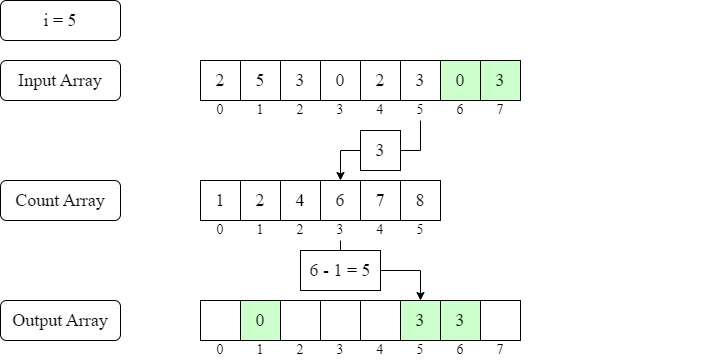
\includegraphics[width=1.0\textwidth]{./assets/images/cs8.jpg}
\end{figure*}
\begin{figure*}[h!]
    \centering
    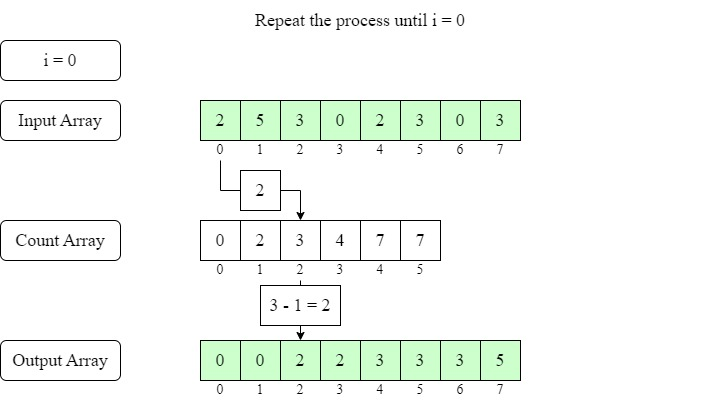
\includegraphics[width=1.0\textwidth]{./assets/images/cs9.jpg}
\end{figure*}
\begin{figure}[h!]
    \centering
    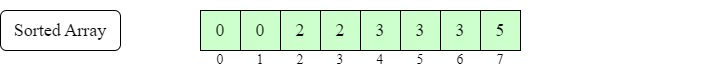
\includegraphics[width=1.0\textwidth]{./assets/images/cs10.jpg}
    \caption{Counting Sort}
    \label{fig:counting-sort}
\end{figure}

Figure \ref{fig:counting-sort} shows the Counting Sort algorithm in 
action. The algorithm sorts an array of elements by counting the
frequency of each distinct element in the input array and placing the
elements in their correct sorted positions based on the count.

\subsubsection{Algorithm of Counting Sort}

\begin{itemize}
    \item Count the frequency of each distinct element in the input array.
    
    \item Calculate the cumulative sum of the frequencies to determine the
    positions of the elements in the sorted array.
    
    \item Place the elements in their correct sorted positions based on the
    count.
\end{itemize}

\subsubsection{Pseudo-code of Counting Sort}

\begin{lstlisting}[caption={Counting Sort Pseudo-code}]
CountingSort(arr)
    N = arr.length
    M = 0

    for i = 0 to N - 1
        M = max(M, arr[i])

    countArray = Array(M + 1, 0)

    for i = 0 to N - 1
        countArray[arr[i]]++

    for i = 1 to M
        countArray[i] += countArray[i - 1]

    outputArray = Array(N)

    for i = N - 1 down to 0
        outputArray[countArray[arr[i]] - 1] = arr[i]
        countArray[arr[i]]--

    return outputArray
\end{lstlisting}

Pseudo-code for Counting Sort is shown in the code snippet. The
algorithm takes an array of elements as input and sorts the array using
the Counting Sort technique. The algorithm counts the frequency of each
distinct element in the input array, calculates the cumulative sum of
the frequencies, and then places the elements in their correct sorted
positions based on the count.

\subsubsection{Counting Sort in C++}

\begin{lstlisting}[language=C++, caption={Counting Sort in C++}, label={lst:counting-sort-cpp}]
#include <iostream>
#include <vector>
using namespace std;

vector<int> countingSort(vector<int> &inputArray) {
    int N = inputArray.size();

    int M = 0;

    for (int i = 0; i < N; i++) {
        M = max(M, inputArray[i]);
    }

    vector<int> countArray(M + 1, 0);

    for (int i = 0; i < N; i++) {
        countArray[inputArray[i]]++;
    }

    for (int i = 1; i <= M; i++) {
        countArray[i] += countArray[i - 1];
    }

    vector<int> outputArray(N);

    for (int i = N - 1; i >= 0; i--) {
        outputArray[countArray[inputArray[i]] - 1] = inputArray[i];
        countArray[inputArray[i]]--;
    }

    return outputArray;
}

void printArray(vector<int> &arr) {
    for (int i = 0; i < arr.size(); i++) {
        cout << arr[i] << " ";
    }
    cout << endl;
}

int main() {
    vector<int> arr = {2, 5, 3, 0, 2, 3, 0, 3};

    cout << "Original Array: ";
    printArray(arr);

    vector<int> sortedArray = countingSort(arr);

    cout << "Sorted Array: ";
    printArray(sortedArray);

    return 0;
}
\end{lstlisting}

Code \ref{lst:counting-sort-cpp} shows the implementation of the Counting
Sort algorithm in C++. The code snippet defines a function
\texttt{countingSort} that takes a vector of integers as input and sorts
the array using the Counting Sort technique. The algorithm counts the
frequency of each distinct element in the input array, calculates the
cumulative sum of the frequencies, and then places the elements in their
correct sorted positions based on the count. In the example, the 
Counting Sort algorithm is used to sort an array of elements, and the
sorted array is printed to the console.

\subsubsection{Advantages and Disadvantages of Counting Sort}

\textbf{Advantages}:

\begin{itemize}
    \item Counting Sort generally performs faster than all comparison-based
    sorting algorithms, such as Merge Sort and Quick Sort, if the range of
    input is of the order of the number of input.
    
    \item Counting Sort is easy to code and implement due to its simple
    counting and placement mechanism.
    
    \item Counting Sort is a stable sorting algorithm that maintains the
    relative order of equal elements in the input array.
\end{itemize}

\textbf{Disadvantages}:

\begin{itemize}
    \item Counting Sort doesn't work on decimal values or floating-point
    numbers, as it requires integer values for counting and placement.
    
    \item Counting Sort is inefficient if the range of values to be sorted
    is very large compared to the number of elements in the input array.
    
    \item Counting Sort is not an in-place sorting algorithm, as it uses
    extra space for counting and placing the array elements in their
    correct sorted positions.
\end{itemize}

\subsubsection{Complexity Analysis of Counting Sort}

The time complexity of Counting Sort is \texttt{$O(n + m)$}, where $n$
is the number of elements in the input array and $m$ is the range of
input values. The space complexity of Counting Sort is \texttt{$O(n + m)$}
due to the additional space required for counting and placing the array
elements in their correct sorted positions.

\subsection{Radix Sort}

Radix Sort is a non-comparison-based sorting algorithm that sorts
elements based on their individual digits or characters. The basic idea
behind Radix Sort is to sort the input array digit by digit, starting
from the least significant digit to the most significant digit. Radix
Sort is particularly efficient for sorting integers or strings with a
fixed length.

% TikZ code for Radix Sort
\begin{figure*}[h!]
    \centering
    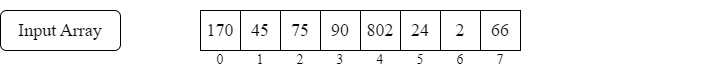
\includegraphics[width=1.0\textwidth]{./assets/images/rs1.jpg}
\end{figure*}
\begin{figure*}[h!]
    \centering
    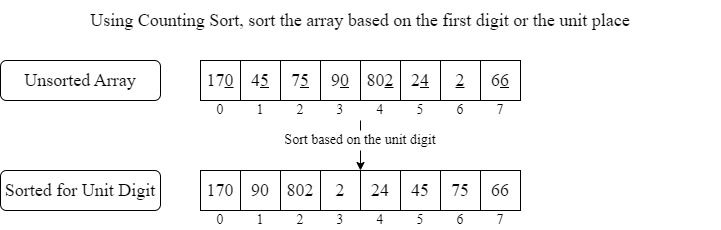
\includegraphics[width=1.0\textwidth]{./assets/images/rs2.jpg}
\end{figure*}
\begin{figure*}[h!]
    \centering
    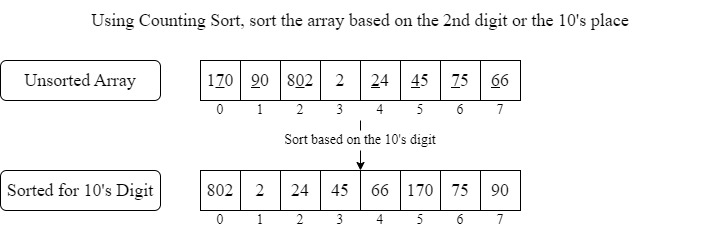
\includegraphics[width=1.0\textwidth]{./assets/images/rs3.jpg}
\end{figure*}
\begin{figure*}[h!]
    \centering
    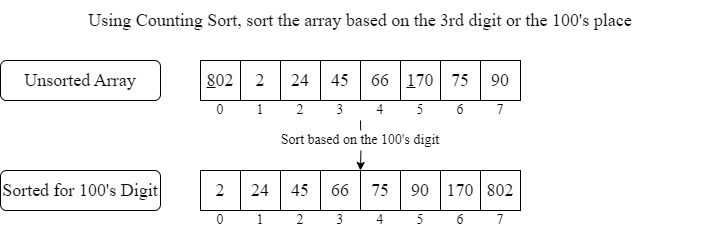
\includegraphics[width=1.0\textwidth]{./assets/images/rs4.jpg}
\end{figure*}
\begin{figure}[h!]
    \centering
    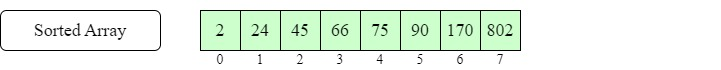
\includegraphics[width=1.0\textwidth]{./assets/images/rs5.jpg}
    \caption{Radix Sort}
    \label{fig:radix-sort}
\end{figure}

Figure \ref{fig:radix-sort} shows the Radix Sort algorithm in action.
The algorithm sorts an array of integers by sorting the elements digit
by digit, starting from the least significant digit to the most
significant digit. In each step, the algorithm uses a stable sorting
algorithm like Counting Sort to sort the elements based on each digit.
The algorithm applies Couting Sort to sort the elements based on the
current digit, and then repeats the process for each digit until the
entire array is sorted.

\subsubsection{Algorithm of Radix Sort}

\begin{itemize}
    \item Sort the input array digit by digit, starting from the least
    significant digit to the most significant digit.
    
    \item Use a stable sorting algorithm like Counting Sort or Bucket Sort
    to sort the elements based on each digit.
    
    \item Repeat the process for each digit until the entire array is
    sorted.
\end{itemize}

\subsubsection{Pseudo-code of Radix Sort}

\begin{lstlisting}[caption={Radix Sort Pseudo-code}]
GetMax(arr, n)
    max_val = arr[0]
    for i = 1 to n - 1
        if arr[i] > max_val
            max_val = arr[i]
    return max_val

CountingSort(arr, n, exp)
    output = Array(n)
    count = Array(10, 0)

    for i = 0 to n - 1
        count[(arr[i] / exp) % 10]++

    for i = 1 to 9
        count[i] += count[i - 1]

    for i = n - 1 down to 0
        output[count[(arr[i] / exp) % 10] - 1] = arr[i]
        count[(arr[i] / exp) % 10]--

    for i = 0 to n - 1
        arr[i] = output[i]

RadixSort(arr)
    n = arr.length
    max_val = GetMax(arr, n)

    for exp = 1 to max_val
        CountingSort(arr, n, exp)
\end{lstlisting}

Pseudo-code for Radix Sort is shown in the code snippet. The algorithm
takes an array of integers as input and sorts the array using the Radix
Sort technique. The algorithm sorts the input array digit by digit,
starting from the least significant digit to the most significant digit,
using a stable sorting algorithm like Counting Sort or Bucket Sort to
sort the elements based on each digit.

\subsubsection{Radix Sort in C++}

\begin{lstlisting}[language=C++, caption={Radix Sort in C++}, label={lst:radix-sort-cpp}]
#include <iostream>
#include <vector>
using namespace std;

int getMax(vector<int> &arr, int n) {
    int max_val = arr[0];
    for (int i = 1; i < n; i++) {
        if (arr[i] > max_val) {
            max_val = arr[i];
        }
    }
    return max_val;
}

void countingSort(vector<int> &arr, int n, int exp) {
    vector<int> output(n);
    vector<int> count(10, 0);

    for (int i = 0; i < n; i++) {
        count[(arr[i] / exp) % 10]++;
    }

    for (int i = 1; i < 10; i++) {
        count[i] += count[i - 1];
    }

    for (int i = n - 1; i >= 0; i--) {
        output[count[(arr[i] / exp) % 10] - 1] = arr[i];
        count[(arr[i] / exp) % 10]--;
    }

    for (int i = 0; i < n; i++) {
        arr[i] = output[i];
    }
}

void radixSort(vector<int> &arr) {
    int n = arr.size();
    int max_val = getMax(arr, n);

    for (int exp = 1; max_val / exp > 0; exp *= 10) {
        countingSort(arr, n, exp);
    }
}

void printArray(vector<int> &arr) {
    for (int i = 0; i < arr.size(); i++) {
        cout << arr[i] << " ";
    }
    cout << endl;
}

int main() {
    vector<int> arr = {170, 45, 75, 90, 802, 24, 2, 66};

    cout << "Original Array: ";
    printArray(arr);

    radixSort(arr);

    cout << "Sorted Array: ";
    printArray(arr);

    return 0;
}
\end{lstlisting}

Code \ref{lst:radix-sort-cpp} shows the implementation of the Radix Sort
algorithm in C++. The code snippet defines a function \texttt{radixSort}
that takes a vector of integers as input and sorts the array using the
Radix Sort technique. The algorithm sorts the input array digit by digit,
starting from the least significant digit to the most significant digit,
using a stable sorting algorithm like Counting Sort to sort the elements
based on each digit. In the example, the Radix Sort algorithm is used to
sort an array of integers, and the sorted array is printed to the console.

\subsubsection{Advantages and Disadvantages of Radix Sort}

\textbf{Advantages}:

\begin{itemize}
    \item Radix Sort is a stable sorting algorithm that maintains the
    relative order of equal elements in the input array.
    
    \item Radix Sort is efficient for sorting integers or strings with a
    fixed length, as it sorts the elements digit by digit.
    
    \item Radix Sort has a time complexity of \texttt{$O(nk)$}, where $n$
    is the number of elements in the input array and $k$ is the number of
    digits or characters in the input values.
\end{itemize}

\textbf{Disadvantages}:

\begin{itemize}
    \item Radix Sort is not suitable for sorting floating-point numbers or
    strings with varying lengths, as it requires fixed-length input values.
    
    \item Radix Sort is not an in-place sorting algorithm, as it uses extra
    space for counting and placing the array elements in their correct
    sorted positions.
    
    \item Radix Sort is not as efficient as comparison-based sorting
    algorithms like Merge Sort or Quick Sort for general-purpose sorting
    tasks.
\end{itemize}

\subsubsection{Complexity Analysis of Radix Sort}

The time complexity of Radix Sort is \texttt{$O(nk)$}, where $n$ is the
number of elements in the input array and $k$ is the number of digits or
characters in the input values. The space complexity of Radix Sort is
\texttt{$O(n + k)$} due to the additional space required for counting
and placing the array elements in their correct sorted positions.

\section{Summary}

In this chapter, we discussed comparison-based and non-comparison-based
sorting algorithms. We explored various sorting algorithms, including
Bubble Sort, Selection Sort, Insertion Sort, Merge Sort, Quick Sort,
Heap Sort, Counting Sort, and Radix Sort. We examined the algorithms,
pseudo-code, implementations in C++, advantages, disadvantages, and
complexity analysis of each sorting algorithm. Sorting algorithms are
essential in computer science and play a crucial role in various
applications, such as data processing, information retrieval, and
optimization problems. Understanding the different sorting algorithms
and their properties is fundamental for designing efficient algorithms
and solving real-world problems.

%%%%%%%%%%%%%%%%%%%%%%%%%%%%%%%%%%%%
%%%%%~ NEW CHAPTER STARTS HERE %%%%%
%%%%%%%%%%%%%%%%%%%%%%%%%%%%%%%%%%%%
% \chapter{Hashing}

% \section{Introduction}

% \section{Hash Table}

% \section{Hash Function}

% \section{Collision Resolution Techniques}

% \subsection{Separate Chaining}

% \subsection{Open Addressing}

% \subsubsection{Linear Probing}

% \subsubsection{Quadratic Probing}

% \subsubsection{Double Hashing}

% \section{Complexity Analysis of Hashing}

% \section{Summary}

%%%%%%%%%%%%%%%%%%%%%%%%%%%%%%%%%%%%
%%%%%~ NEW CHAPTER STARTS HERE %%%%%
%%%%%%%%%%%%%%%%%%%%%%%%%%%%%%%%%%%%
% \chapter{Advanced Data Structures and Algorithms}

% \section{Introduction}

% \section{Advanced Data Structures}

% \subsection{Segment Tree}

% \subsection{Fenwick Tree}

% \subsection{Suffix Tree}

% \subsection{Suffix Array}

% \subsection{Trie}

% \subsection{Heap}

% \subsection{Disjoint Set}

% \subsection{Skip List}

% \subsection{Splay Tree}

% \subsection{Bloom Filter}

% \subsection{KD Tree}

% \subsection{Quad Tree}

% \subsection{Octree}

% \subsection{B-Tree}

% \subsection{B+ Tree}

% \subsection{R-Tree}

% \subsection{X-Tree}

% \subsection{Y-Tree}

% \subsection{Z-Tree}

% \section{Advanced Algorithms}

% \subsection{Dynamic Programming}

% \subsection{Greedy Algorithms}

% \subsection{Backtracking}

% \subsection{Divide and Conquer}

% \subsection{Branch and Bound}

% \subsection{Randomized Algorithms}

% \subsection{Approximation Algorithms}

% \subsection{String Matching Algorithms}

% \subsection{Pattern Searching Algorithms}

% \subsection{Cryptography Algorithms}

% \subsection{Geometric Algorithms}

% \subsection{Graph Algorithms}

% \subsection{Network Flow Algorithms}

% \subsection{Game Theory Algorithms}

% \subsection{Quantum Algorithms}

% \section{Summary}

%%%%%%%%%%%%%%%%%%%%%%%%%%%%%%%%%%%%
%%%%%~ NEW CHAPTER STARTS HERE %%%%%
%%%%%%%%%%%%%%%%%%%%%%%%%%%%%%%%%%%%
% \chapter{Applications of Data Structures and Algorithms}

% \section{Applications in Computer Science}

% \subsection{Operating Systems}

% \subsection{Database Management Systems}

% \subsection{Compiler Design}

% \subsection{Networking}

% \subsection{Artificial Intelligence}

% \subsection{Machine Learning}

% \subsection{Computer Graphics}

% \subsection{Computer Vision}

% \subsection{Robotics}

% \subsection{Web Development}

% \subsection{Mobile Development}

% \subsection{Game Development}

% \subsection{Cybersecurity}

% \subsection{Quantum Computing}

% \section{Applications in Real Life}

% \subsection{Social Media}

% \subsection{E-commerce}

% \subsection{Healthcare}

% \subsection{Finance}

% \subsection{Transportation}

% \subsection{Education}

% \subsection{Agriculture}

% \subsection{Manufacturing}

% \subsection{Entertainment}

% \subsection{Sports}

% \subsection{Travel}

% \subsection{Telecommunications}

% \subsection{Energy}

% \subsection{Environment}

% \subsection{Politics}

% \subsection{Military}

% \section{Summary}

\chapter{References}

\begin{enumerate}[label={\textbf{\Alph*.}}]
  \item \textbf{Books}
    \begin{itemize}
      \item Vishwas R. (2023). Data Structure Handbook. Dr. Vishwas Raval. ISBN: 978-9359063591
      \item Cormen, T. H., Leiserson, C. E., Rivest, R. L., \& Stein, C. (2022). Introduction to algorithms. MIT press. ISBN: 978-0262046305
      \item Erickson, J. (2019). Algorithms. ISBN: 978-1792644832
    \end{itemize}
  \item \textbf{Other Sources}
    \begin{itemize}
      \item Tutorialspoint. (n.d.). Data Structures Basics. Data Structure Basics. \url{https://www.tutorialspoint.com/data_structures_algorithms/data_structures_basics.htm}
      \item Algorithm Archive · Arcane Algorithm Archive. (n.d.). \url{https://www.algorithm-archive.org/}
    \end{itemize}
\end{enumerate}

\end{document}
